\documentclass[a4paper,11pt]{report}

% Packages
\usepackage[utf8]{inputenc}
\usepackage[T1]{fontenc}
\usepackage[ngerman]{babel} % For German language
\usepackage{graphicx}
\usepackage{amsmath}
\usepackage{amsfonts}
\usepackage{amssymb}
\usepackage{hyperref}
\usepackage{listings} % For code listings
\usepackage{setspace} % For line spacing
\usepackage{geometry} % For setting margins
\usepackage{titlesec} % For customizing title formats
\usepackage{chngcntr} % For changing counter settings
\usepackage{fancyhdr} % For custom headers and footers
\usepackage[style=ieee,backend=biber,url=true,citestyle=numeric-comp]{biblatex}
\addbibresource{references.bib}
% Remove empty parenthesis if no date specified 
\DeclareFieldFormat{parens}{%
  \iffieldundef{year}{}{\mkbibparens{#1}}%
}
\DeclareFieldFormat{date}{%
  \iffieldundef{year}{n.d.}{#1}%
}

\usepackage{float}
\usepackage{titling}
\usepackage{svg}
\usepackage{pdfpages}
\usepackage{array}
\usepackage{acro}
\usepackage{csquotes}
\usepackage{url}
\usepackage{breakurl}
\usepackage[export]{adjustbox}
\usepackage{booktabs}
\usepackage{longtable}
%\newcolumntype{P}[1]{>{\raggedright\arraybackslash}p{#1}}
\usepackage{tabularx}  % Automatically adjusts table width
\usepackage{hyperref}
\usepackage{subcaption}
\usepackage{xcolor}
\usepackage{siunitx}
\usepackage{listings}
\usepackage{dirtree}
\usepackage{textgreek}

\lstdefinelanguage{json}{
    morestring=[b]",
    morecomment=[l]{//},
    morekeywords={true, false, null},
    sensitive=false,
}

\lstset{
    language=json,
    backgroundcolor=\color{gray!10},
    basicstyle=\ttfamily\small,
    keywordstyle=\color{blue},
    stringstyle=\color{orange},
    commentstyle=\color{gray},
    showstringspaces=false,
    breaklines=true
}

% Margins
\geometry{
    left=3cm,
    right=2.5cm,
    top=2.5cm,
    bottom=2.5cm
}

% Line spacing
\onehalfspacing % 1.5 line spacing, you can use \singlespacing for single line spacing

% Remove ident before newline
\setlength{\parindent}{0pt}

% Decimal numbering without "Kapitel" prefix
\titleformat{\chapter}[block]
  {\normalfont\huge\bfseries}{\thechapter.}{20pt}{\Large}
\titleformat{\section}
  {\normalfont\Large\bfseries}{\thesection.}{1em}{}
\titleformat{\subsection}
  {\normalfont\large\bfseries}{\thesubsection.}{1em}{}
\titleformat{\subsubsection}
  {\normalfont\normalsize\bfseries}{\thesubsubsection.}{1em}{}

% Custom headers
\pagestyle{fancy}
\fancyhf{}
\fancyhead[L]{\leftmark}    % Left side of the header
\fancyfoot[C]{\thepage}     % Mid side of the footer

% Redefine \leftmark to show only the chapter number and title
\renewcommand{\chaptermark}[1]{\markboth{\thechapter.\ #1}{}}

% \input{acronyms.tex}

\begin{document}

% Title Page
\begin{titlepage}
    \begin{flushleft}
        
\includegraphics[width=.6\textwidth]{./images/oth.png}
    \end{flushleft}

    \vspace*{2cm}

    \centering
    {\scshape\Large Datenverarbeitung in der Technik \par}
    \vspace{0.5cm}
    {\scshape Sommersemester 2025 \par}
    \vspace{0.5cm}
    {\huge\bfseries Projektbericht \par}
    \vspace{3cm}

    \begin{flushleft}
        \large
        \textbf{Teammitglieder:} \\
        \vspace{0.5cm}

        Fabian Becker\hfill\makebox[8cm]{\hrulefill} \\[0.5cm]
        Jendrik Jürgens\hfill\makebox[8cm]{\hrulefill} \\[0.5cm]
        Nicolas Koch\hfill\makebox[8cm]{\hrulefill} \\[0.5cm]
        Michael Specht\hfill\makebox[8cm]{\hrulefill} \\[0.5cm]
        Jonathan Wohlrab\hfill\makebox[8cm]{\hrulefill} \\[1cm]

        \textbf{Betreuung:} \\
        Dr. Alexander Metzner, Matthias Altmann \\
        \vspace{0.5cm}

        \textbf{Abgabedatum:} \\
        15.07.2025 \\
    \end{flushleft}

    \vfill
    \centering
    {\large \today\par}
\end{titlepage}


% Table of Contents
\tableofcontents
\newpage

% Main Content
\chapter{Projektplanung}

\section{Definiton (Wohlrab)}

Die anfänglichen Überlegungen zum Projekt beschäftigten sich mit dem grundlegenden Aufbau des Systems.
Dazu haben wir zunächst alle Funktionen und die dafür benötigten Komponenten zusammengestellt.
Anschließend haben wir überlegt, wie sich die verschiedenen Komponenten miteinander verbinden lassen und welche von welchen Mikrocontrollern gesteuert werden sollen.
Dabei hat sich eine Zweiteilung des Systems ergeben: 
\begin{itemize}
    \item Wir wollten alle Motoren und Servos mit einem ESP32 verbinden.
    Dieser sollte außerdem über eine Bluetooth-Verbindung die Steuerbefehle des PlayStation-Controllers entgegennehmen.
    \item Die gesamte Sensorik des Systems soll über einen Raspberry Pi 5 ausgewertet werden.
    Er sammelt und kombiniert die Informationen aus den Sensorwerten und verarbeitet sie mithilfe eines KI-Modells.
    Dabei sollen Ziele über die Kamera erkannt und ihre Position mithilfe der weiteren Sensoren bestimmt werden.
    Auf dieser Grundlage sollen Steuerungsbefehle für den ESP32 berechnet und an diesen weitergegeben werden.
    Das Video der Kamera soll zudem über einen Webserver dargestellt werden.
\end{itemize}

\section{GANTT-Diagram (Wohlrab)}

Zu Beginn wird eine vollständige Auflistung aller für das Projekt relevanten Komponenten erstellt. 
Aus diesen Komponenten werden die entsprechenden Arbeitspakete abgeleitet.
Im nächsten Schritt erfolgt eine fundierte Abschätzung des Umfangs der einzelnen Arbeitspakete. 
Mithilfe dieser Schätzung wird der zeitliche Aufwand für die Bearbeitung jedes Pakets ermittelt.
Zur besseren Übersichtlichkeit werden die zeitlichen Abhängigkeiten zwischen den Arbeitspaketen dargestellt. 
Diese Darstellung ermöglicht es, die Reihenfolge der Aufgaben und ihre Zusammenhänge zu visualisieren. 
Dadurch wird eine effiziente und systematische Arbeitsweise gewährleistet.
Die Arbeitspakete werden anschließend auf die Gruppenmitglieder verteilt, wobei darauf geachtet wird, dass die Gesamtaufwände innerhalb des Teams ausgewogen sind. 
Dies trägt dazu bei, die Arbeitslast gerecht zu verteilen und die Effektivität des Teams zu maximieren.
Zur besseren Differenzierung sind die verschiedenen Arten von Arbeitspaketen im Diagramm farblich gekennzeichnet.

\section{Lastenheft (Wohlrab)}

Das Lastenheft stellt ein zentrales Dokument im Projektmanagement dar, da es die Anforderungen und Ziele des Projekts formell festhält. 
Es dient der präzisen Definition des Projektumfangs und legt den Rahmen fest, innerhalb dessen das Projekt durchgeführt wird. 
Durch die detaillierte Beschreibung der zu erfüllenden Anforderungen und Zielsetzungen gibt das Lastenheft eine klare Orientierung und leitet alle nachfolgenden Tätigkeiten ab. 
Nach Abschluss des Projekts ermöglicht es zudem eine objektive Beurteilung des Projekterfolgs, da es als Grundlage für die Evaluation der erreichten Ergebnisse und der Zielerreichung dient.

\section{Plakat (Wohlrab)}

Das Plakat ist ein zentrales Element der visuellen Kommunikation des Projekts, da es die wesentlichen Inhalte auf ansprechende Weise veranschaulicht. 
Ziel ist es, das Interesse von Personen zu wecken und ihnen eine schnelle, aber umfassende Übersicht über das Projekt zu vermitteln. 
Der Fokus liegt dabei auf den Hauptfunktionen des Projekts. 
Eine vollständige Aufstellung aller Funktionen wird bewusst vermieden, um die Aufmerksamkeit auf die Schlüsselaspekte zu lenken. 
Das Plakat ist somit ein effektives Kommunikationsmittel, das die wichtigsten Informationen auf klare Weise darstellt.


\chapter{Stromversorgung}

\section{Analyse des Aufbaus und der Komponenten des vorherigen Projekts (Koch)}

Zu Beginn wurde die bestehende Stromversorgung und die dafür genutzten Komponenten eines früheren Semesterprojekts analysiert, um anhand dessen bestimmen zu können, welche Teile wiederverwendet werden können, sowie ob das gegebene Layout in etwa für das eigene Projekt genutzt werden kann.

Essentiell bestand die Stromversorgung aus zwei Step-Down-Wandlern, die aus einer Eingangsspannung eine 8V und eine 5V Ausgangsspannung erzeugten, was ebenfalls für unser eigenes Projekt benötigt wird. Außerdem wurden zwei Verteiler genutzt, um die Spannungen auf die verschiedenen Sensoren und Aktoren zu verteilen.
Das vorhandene Layout auf dem Lochrastergerüst war für uns jedoch nicht geeignet, da wir einen übersichtlicheren Aufbau und ein sinnvolles Color-Coding der Kabel für die verschiedenen Anschlüsse und für einen besseren Überblick anstrebten.

\section{Aufbau der eigenen Stromversorgung (Koch)}
Nachdem die vorhandenen Teile analysiert wurden, wurde die Entscheidung getroffen nur die Step-Down-Wandler, da der Rest nicht relevant für unser Projekt war. Lediglich die Verteiler brauchten wir auch, mussten allerdings ersetzt werden, da die Schraubverbindungen kaputt waren.
Die Step-Down-Wandler waren so aufgebaut, dass ein Modul die Eingangsspannung erhielt und am Ausgang ein selbstangefertigtes Y-Kabel hatte, welches dann jeweils in einen Verteiler und in den anderen Step-Down-Wandler ging.
Diese Kombination sollte auch so für unser Projekt übernommen werden, allerdings mussten dafür die Kabel erneuert werden, da die alten Kabel nicht dem geplanten Color-Coding entsprachen und zu kurz waren. Dabei stellte sich heraus, dass der entstandene Durchmesser, durch die Kombination aus zwei Kabeln zu einem Y-Kabel, zu groß war, um in die Steckverbindung zu passen.
Aus diesem Grund entstand das alternative Konzept die ausgehenden Kabel des ersten Step-Down-Wandlers mit dem ersten Verteiler zu verbinden. Das war vor allem dadurch leicht realisierbar, da jeder Verteiler 12 Ports besitzt und 8V lediglich für die Motoren zum fahren benötigt werden. Somit konnte eine Verbindung vom 8V-Verteiler zum zweiten Step-Down-Wanlder hergestellt werden ohne dabei die Steckverbindungen zu beschädigen.
\newpage
Das Color-Coding der Kabel wurde wie folgt eingeführt:
\begin{itemize}
    \item \textbf{Rot:} Versorgungsspannung
    \item \textbf{Schwarz:} Masse
    \item \textbf{Weiß:} PWM-Verbindung für Motoren
    \item \textbf{Gelb:} Direction Pin für Motoren
\end{itemize}
Des Weiteren wurde darauf geachtet, dass die Kabel so kurz wie möglich gehalten werden und wenn möglich unter der Platte verlegt werden, um eine bessere Übersicht zu gewährleisten.

Als Eingangsspannung wurde zu Beginn ein 6V-Batterieverbund genutzt, der im Laufe des Projekts durch einen 12V-Batterieverbund ausgetauscht wurde, da beim Testing der Motortreiber festgestellt wurde, dass die Motoren eine höhere Spannung benötigen, um korrekt zu funktionieren. Außerdem wurde versucht den Raspberry Pi 5 über den 5V-Verteiler zu versorgen, was jedoch nicht funktionierte, da die Stromstärke zu niedrig war, wenn der Pi aufwendigere Aufgaben erledigen musste. Aus diesem Grund wurde eine Powerbank genutzt, die den Pi mit Strom versorgt und somit die 5V-Verteilung entlastet.

Der Gesamtaufbau der Stromversorgung sieht dabei wie folgt aus:
\begin{itemize}
    \item \textbf{12V-Batterieverbund:}
    \begin{itemize}
        \item Step-Down-Wandler (8V) $\rightarrow$ 8V-Verteiler
        \begin{itemize}
            \item 2 PWM Boards für Motoren
            \item Step-Down-Wandler (5V) $\rightarrow$ 5V-Verteiler
            \begin{itemize}
                \item ESP32
                \item 2 PWM Boards für die Flywheel Motoren
                \item Servo-Motor für die Geschützplattform
                \item Servo-Motor für den Geschützarm
            \end{itemize}
        \end{itemize}
    \end{itemize}
    
    \item \textbf{Powerbank:}
    \begin{itemize}
        \item Raspberry Pi 5
        \begin{itemize}
            \item Pi-Camera
            \item MPU6050 Gyrosensor
            \item SRF02 Ultraschallsensor
        \end{itemize}
    \end{itemize}
\end{itemize}
\chapter{Stromversorgung}

\section{Analyse des Aufbaus und der Komponenten des vorherigen Projekts (Koch)}

Zu Beginn wurde die bestehende Stromversorgung und die dafür genutzten Komponenten eines früheren Semesterprojekts analysiert, um anhand dessen bestimmen zu können, welche Teile wiederverwendet werden können, sowie ob das gegebene Layout in etwa für das eigene Projekt genutzt werden kann.

Essentiell bestand die Stromversorgung aus zwei Step-Down-Wandlern, die aus einer Eingangsspannung eine 8V und eine 5V Ausgangsspannung erzeugten, was ebenfalls für unser eigenes Projekt benötigt wird. Außerdem wurden zwei Verteiler genutzt, um die Spannungen auf die verschiedenen Sensoren und Aktoren zu verteilen.
Das vorhandene Layout auf dem Lochrastergerüst war für uns jedoch nicht geeignet, da wir einen übersichtlicheren Aufbau und ein sinnvolles Color-Coding der Kabel für die verschiedenen Anschlüsse und für einen besseren Überblick anstrebten.

\section{Aufbau der eigenen Stromversorgung (Koch)}
Nachdem die vorhandenen Teile analysiert wurden, wurde die Entscheidung getroffen nur die Step-Down-Wandler, da der Rest nicht relevant für unser Projekt war. Lediglich die Verteiler brauchten wir auch, mussten allerdings ersetzt werden, da die Schraubverbindungen kaputt waren.
Die Step-Down-Wandler waren so aufgebaut, dass ein Modul die Eingangsspannung erhielt und am Ausgang ein selbstangefertigtes Y-Kabel hatte, welches dann jeweils in einen Verteiler und in den anderen Step-Down-Wandler ging.
Diese Kombination sollte auch so für unser Projekt übernommen werden, allerdings mussten dafür die Kabel erneuert werden, da die alten Kabel nicht dem geplanten Color-Coding entsprachen und zu kurz waren. Dabei stellte sich heraus, dass der entstandene Durchmesser, durch die Kombination aus zwei Kabeln zu einem Y-Kabel, zu groß war, um in die Steckverbindung zu passen.
Aus diesem Grund entstand das alternative Konzept die ausgehenden Kabel des ersten Step-Down-Wandlers mit dem ersten Verteiler zu verbinden. Das war vor allem dadurch leicht realisierbar, da jeder Verteiler 12 Ports besitzt und 8V lediglich für die Motoren zum fahren benötigt werden. Somit konnte eine Verbindung vom 8V-Verteiler zum zweiten Step-Down-Wanlder hergestellt werden ohne dabei die Steckverbindungen zu beschädigen.
\newpage
Das Color-Coding der Kabel wurde wie folgt eingeführt:
\begin{itemize}
    \item \textbf{Rot:} Versorgungsspannung
    \item \textbf{Schwarz:} Masse
    \item \textbf{Weiß:} PWM-Verbindung für Motoren
    \item \textbf{Gelb:} Direction Pin für Motoren
\end{itemize}
Des Weiteren wurde darauf geachtet, dass die Kabel so kurz wie möglich gehalten werden und wenn möglich unter der Platte verlegt werden, um eine bessere Übersicht zu gewährleisten.

Als Eingangsspannung wurde zu Beginn ein 6V-Batterieverbund genutzt, der im Laufe des Projekts durch einen 12V-Batterieverbund ausgetauscht wurde, da beim Testing der Motortreiber festgestellt wurde, dass die Motoren eine höhere Spannung benötigen, um korrekt zu funktionieren. Außerdem wurde versucht den Raspberry Pi 5 über den 5V-Verteiler zu versorgen, was jedoch nicht funktionierte, da die Stromstärke zu niedrig war, wenn der Pi aufwendigere Aufgaben erledigen musste. Aus diesem Grund wurde eine Powerbank genutzt, die den Pi mit Strom versorgt und somit die 5V-Verteilung entlastet.

Der Gesamtaufbau der Stromversorgung sieht dabei wie folgt aus:
\begin{itemize}
    \item \textbf{12V-Batterieverbund:}
    \begin{itemize}
        \item Step-Down-Wandler (8V) $\rightarrow$ 8V-Verteiler
        \begin{itemize}
            \item 2 PWM Boards für Motoren
            \item Step-Down-Wandler (5V) $\rightarrow$ 5V-Verteiler
            \begin{itemize}
                \item ESP32
                \item 2 PWM Boards für die Flywheel Motoren
                \item Servo-Motor für die Geschützplattform
                \item Servo-Motor für den Geschützarm
            \end{itemize}
        \end{itemize}
    \end{itemize}
    
    \item \textbf{Powerbank:}
    \begin{itemize}
        \item Raspberry Pi 5
        \begin{itemize}
            \item Pi-Camera
            \item MPU6050 Gyrosensor
            \item SRF02 Ultraschallsensor
        \end{itemize}
    \end{itemize}
\end{itemize}

\chapter{CAD-Konstruktion}

\section{Setup und Einarbeitung (Becker, Specht)}

Zu Beginn des Projekts wurde in Abstimmung mit Fabian Becker sowie im Austausch mit Andreas Wittmann (Studienkollege) entschieden, FreeCAD als CAD-Software zu verwenden. Der Grund hierfür war die einfache Kollaboration innerhalb der Projektgruppe sowie der unkomplizierte Erfahrungsaustausch mit der Arbeitsgruppe um A. Wittmann. Andere Softwarelösungen wie OnShape wurden diskutiert, aufgrund der Komplexität und der damit verbundenen Einarbeitungszeit im Hinblick auf die Projektlaufzeit jedoch verworfen. FreeCAD ist zudem eine Open-Source-Software, die neben Fedora auch auf Debian-Systemen lauffähig ist. So konnte die Software problemlos auf den Arbeitsrechnern der Teammitglieder installiert werden.

Grundsätzlich stützt sich die Konstruktion auf vorhandene STL-Vorlagen. Ein Beispielprojekt aus dem Internet diente als Grundlage für die Arbeit.

\section{Geschützarm Version 1 (Specht) \label{sec:cad_gunarm_v1}}

Bevor mit der Konstruktion begonne wurde, wurde im Team besprochen, welche Komponenten nötig sind, um die Position des Flugobjekts eindeutig zu bestimmen. Die Wahl fiel auf folgende Komponenten, die aus vorherigen Studienprojekten übernommen werden konnten:

\begin{itemize}
    \item GY-521 MPU-6050 3-Achsen-Gyroskop und Beschleunigungssensor
    \item SRF02 Ultraschall Entfernungssensor
    \item Raspberry Pi 5 Kamera Modul
    \item 2x 28BYJ-48 Schrittmotor
\end{itemize}

Ziel des ersten Entwurfs war es, diese kompakt auf dem Arm zu integrieren. Die angedachten Schrittmotoren wichen jedoch von der Vorlage aus dem Beispielprojekt ab, weshalb der Geschützarm von Grund auf neu konstruiert werden musste.

Alle Module sollten zentral über der Abschusseinrichtung platziert werden, um eine korrekte Berechnung der Flugbahn zu ermöglichen. Der Ultraschall-Sensor sollte dabei hochkant nach vorne gerichtet sein, um die Entfernung zum Ziel zu messen. Die Kamera sollte schräg nach oben gerichtet sein, um den Himmel zu überwachen. Der Beschleunigungssensor sollte liegend auf dem Arm montiert werden, um die Beschleunigung des Arms zu messen. Die Schrittmotoren mussten in einem geeigneten Abstand zueinander montiert werden, sodass die Flywheel-Konstruktion des Arms funktioniert. Letzteres konnte durch das Vermessen der Vorlage aus dem Beispielprojekt realisiert werden. Für die restlichen Anforderungen waren die korrekten Maße nötig. Für die Montage der Kamera konnte eine bereits 3D-gedruckte Halterung aus einer anderen Gruppe benutzt werden. Die Haltevorrichtung für den Beschleunigungssensor wurde aus einer STL-Vorlage übernommen und angepasst. Auch für die Schrittmotoren konnte auf ein Modell aus dem Internet zurückgegriffen werden, weshalb es nicht nötig war, die komplexe Geometrie eigenständig zu vermessen. Einzig die Maße für den Ultraschall-Sensor wurden recherchiert und durch Nachmessen validiert.

\begin{figure}[h]
    \centering

    \begin{subfigure}[b]{0.45\textwidth}
        \centering
        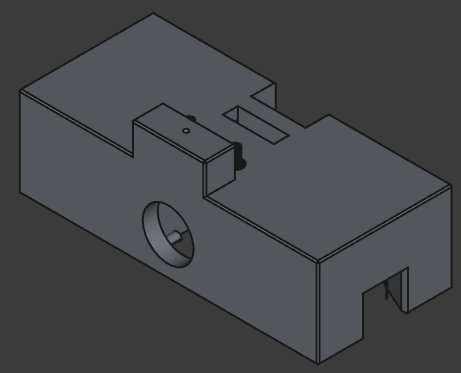
\includegraphics[width=\textwidth]{images/cad_gunarm_v1_front.jpg}
        \caption{Geschützarm Version 1 - Frontansicht}
    \end{subfigure}
    \hfill
    \begin{subfigure}[b]{0.45\textwidth}
        \centering
        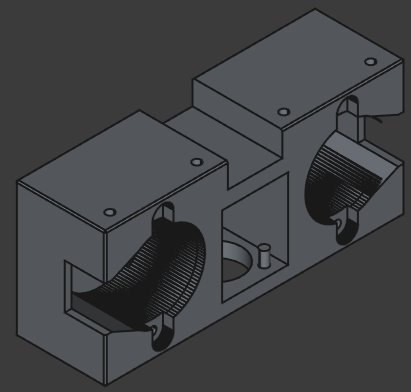
\includegraphics[width=\textwidth]{images/cad_gunarm_v1_back.jpg}
        \caption{Geschützarm Version 1 - Rückansicht}
    \end{subfigure}

    \caption{Geschützarm Version 1}
    \label{fig:gunarm_v1}
\end{figure}

Neben den eigentlichen Maßen der Komponenten war das Kabelmanagement ein wichtiges Thema. Alle Kabel sollten nach hinten am Magazin entlang geführt werden, um eine saubere Optik zu gewährleisten. Für Beschleunigungssensor und Kamera stellte dies kein Problem dar, da diese ganz oben angebracht sein sollten. Der Ultraschall-Sensor und die Schrittmotoren hingegen waren in das neukonstruierte Gehäuse integriert, sodass Aussparungen, wie in Abbildung~\ref{fig:gunarm_v1} zu sehen, angebracht werden mussten, um die Kabel aus dem Gehäuse herauszuführen.

Außerdem musste sichergestellt werden, dass der Geschützarm an das Magazin montiert werden kann. Hierzu wurden vom Kollegen Fabian Becker Montagepunkte am Magazin konstruiert, die mit dem Geschützarm verschraubt werden können.

\section{Geschützarm Version 2 (Specht)}

Im Laufe des Projektes wurde in Abstimmung mit Fabian Becker klar, dass die Schrittmotoren aufgrund zu geringer Leistung nicht für die Flywheel-Konstruktion geeignet sind. Daraufhin wurde sich für die originalen Motoren aus dem Beispielprojekt entschieden. Das hatte zur Folge, dass der Geschützarm neu konstruiert werden musste, da die Maße der neuen Motoren von den Alten abwichen. Aus diesem Grund wurde der Geschützarm der Vorlage als Basis genommen und die Grundidee der Version 1 beibehalten.

\begin{figure}[h]
    \centering

    \begin{subfigure}[b]{0.45\textwidth}
        \centering
        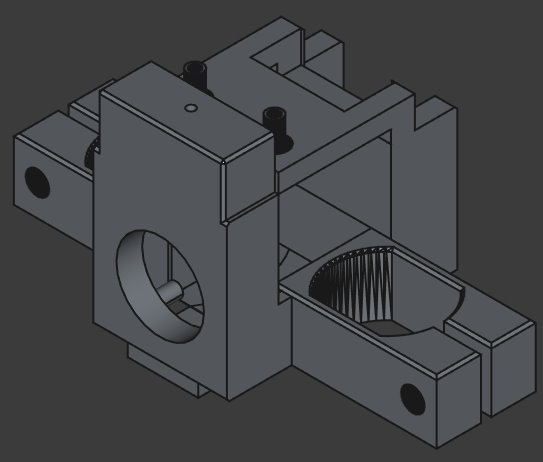
\includegraphics[width=\textwidth]{images/cad_gunarm_v2_front.jpg}
        \caption{Geschützarm Version 2 - Frontansicht}
    \end{subfigure}
    \hfill
    \begin{subfigure}[b]{0.45\textwidth}
        \centering
        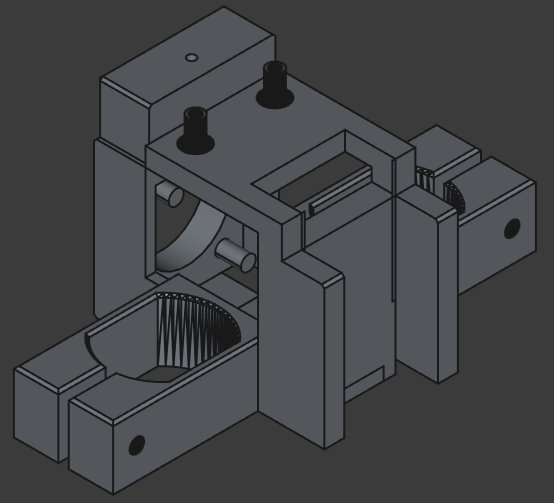
\includegraphics[width=\textwidth]{images/cad_gunarm_v2_back.jpg}
        \caption{Geschützarm Version 2 - Rückansicht}
    \end{subfigure}

    \caption{Geschützarm Version 2}
    \label{fig:gunarm_v2}
\end{figure}

Im Gegensatz zur Version 1 wird der Ultraschallsensor nun seitlich eingeführt anstatt von unten, siehe~\ref{fig:gunarm_v2}. Problematisch waren dabei die beschränkten Platzverhältnisse, da die Schrittmotoren näher am Kanonenrohr angebracht wurden als im vorherigen Entwurf. Außerdem wurden die zuvor angedachten Montagepunkte am Magazin wieder entfernt. Die Zusammenführung des Geschützarms mit dem Magazin erfolgte deshalb mittels Modellbaukleber.

\section{Montagehalterung Motortreiber (Specht)}

Für die ersten Funktionstests wurden die Pololu-Motoren provisorisch auf Kork-Schnipseln montiert. Dieses Vorgehen ermöglichte eine zügige Inbetriebnahme, jedoch erwies es sich hinsichtlich Stabilität und Sicherheit als unzureichend. Im Rahmen der Tests kam es zum Abrutschen eines Motors von der Korkunterlage, was zu einer kurzfristigen Wärmeentwicklung und Geruchsbildung führte. Glücklicherweise wurde eine Beschädigung der Hardware vermieden.

\begin{figure}[h]
    \centering

    \begin{subfigure}[b]{0.25\textwidth}
        \centering
        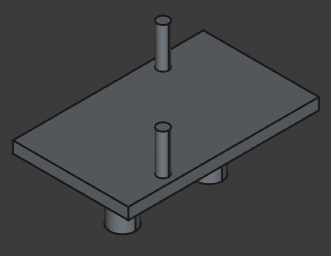
\includegraphics[width=\textwidth]{images/cad_polulu_front.png}
        \caption{Polulu - Draufsicht}
    \end{subfigure}
    \hspace{0.05\textwidth} % Adjust this value as needed
    \begin{subfigure}[b]{0.25\textwidth}
        \centering
        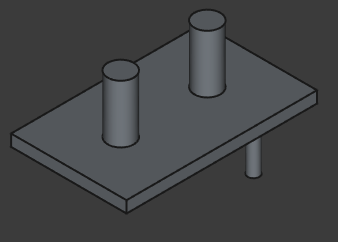
\includegraphics[width=\textwidth]{images/cad_polulu_back.png}
        \caption{Polulu - Bodensicht}
    \end{subfigure}

    \caption{Montagehalterung für Pololu-Motortreiber}
    \label{fig:pololu_mounting}
\end{figure}

Für die finale Abnahme wurde daher ein dauerhaftes und sicheres Montagesystem umgesetzt, das ein sauberes und zuverlässiges Setup gewährleistet. Wie in Abbildung~\ref{fig:pololu_mounting} zu sehen, kann die Halterung direkt auf der Montageplatte des Fahrzeugs geklippt werden.
\chapter{CAD-Konstruktion}

\section{Setup und Einarbeitung (Becker, Specht)}

Zu Beginn des Projekts wurde in Abstimmung mit Fabian Becker sowie im Austausch mit Andreas Wittmann (Studienkollege) entschieden, FreeCAD als CAD-Software zu verwenden. Der Grund hierfür war die einfache Kollaboration innerhalb der Projektgruppe sowie der unkomplizierte Erfahrungsaustausch mit der Arbeitsgruppe um A. Wittmann. Andere Softwarelösungen wie OnShape wurden diskutiert, aufgrund der Komplexität und der damit verbundenen Einarbeitungszeit im Hinblick auf die Projektlaufzeit jedoch verworfen. FreeCAD ist zudem eine Open-Source-Software, die neben Fedora auch auf Debian-Systemen lauffähig ist. So konnte die Software problemlos auf den Arbeitsrechnern der Teammitglieder installiert werden.

Grundsätzlich stützt sich die Konstruktion auf vorhandene STL-Vorlagen. Ein Beispielprojekt aus dem Internet diente als Grundlage für die Arbeit.

\section{Geschützarm Version 1 (Specht) \label{sec:cad_gunarm_v1}}

Bevor mit der Konstruktion begonne wurde, wurde im Team besprochen, welche Komponenten nötig sind, um die Position des Flugobjekts eindeutig zu bestimmen. Die Wahl fiel auf folgende Komponenten, die aus vorherigen Studienprojekten übernommen werden konnten:

\begin{itemize}
    \item GY-521 MPU-6050 3-Achsen-Gyroskop und Beschleunigungssensor
    \item SRF02 Ultraschall Entfernungssensor
    \item Raspberry Pi 5 Kamera Modul
    \item 2x 28BYJ-48 Schrittmotor
\end{itemize}

Ziel des ersten Entwurfs war es, diese kompakt auf dem Arm zu integrieren. Die angedachten Schrittmotoren wichen jedoch von der Vorlage aus dem Beispielprojekt ab, weshalb der Geschützarm von Grund auf neu konstruiert werden musste.

Alle Module sollten zentral über der Abschusseinrichtung platziert werden, um eine korrekte Berechnung der Flugbahn zu ermöglichen. Der Ultraschall-Sensor sollte dabei hochkant nach vorne gerichtet sein, um die Entfernung zum Ziel zu messen. Die Kamera sollte schräg nach oben gerichtet sein, um den Himmel zu überwachen. Der Beschleunigungssensor sollte liegend auf dem Arm montiert werden, um die Beschleunigung des Arms zu messen. Die Schrittmotoren mussten in einem geeigneten Abstand zueinander montiert werden, sodass die Flywheel-Konstruktion des Arms funktioniert. Letzteres konnte durch das Vermessen der Vorlage aus dem Beispielprojekt realisiert werden. Für die restlichen Anforderungen waren die korrekten Maße nötig. Für die Montage der Kamera konnte eine bereits 3D-gedruckte Halterung aus einer anderen Gruppe benutzt werden. Die Haltevorrichtung für den Beschleunigungssensor wurde aus einer STL-Vorlage übernommen und angepasst. Auch für die Schrittmotoren konnte auf ein Modell aus dem Internet zurückgegriffen werden, weshalb es nicht nötig war, die komplexe Geometrie eigenständig zu vermessen. Einzig die Maße für den Ultraschall-Sensor wurden recherchiert und durch Nachmessen validiert.

\begin{figure}[h]
    \centering

    \begin{subfigure}[b]{0.45\textwidth}
        \centering
        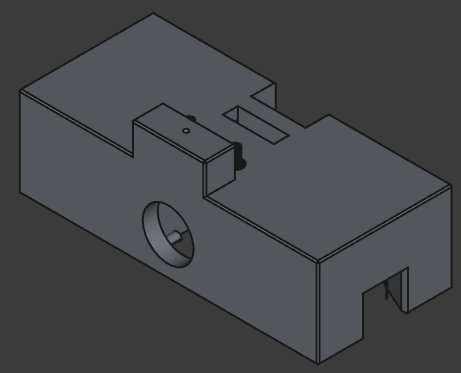
\includegraphics[width=\textwidth]{images/cad_gunarm_v1_front.jpg}
        \caption{Geschützarm Version 1 - Frontansicht}
    \end{subfigure}
    \hfill
    \begin{subfigure}[b]{0.45\textwidth}
        \centering
        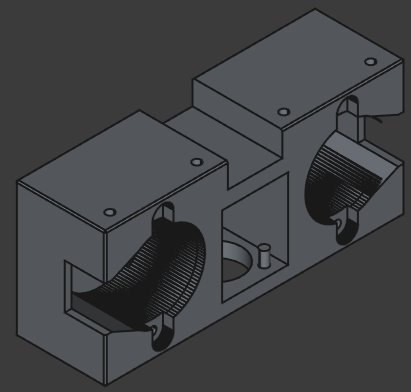
\includegraphics[width=\textwidth]{images/cad_gunarm_v1_back.jpg}
        \caption{Geschützarm Version 1 - Rückansicht}
    \end{subfigure}

    \caption{Geschützarm Version 1}
    \label{fig:gunarm_v1}
\end{figure}

Neben den eigentlichen Maßen der Komponenten war das Kabelmanagement ein wichtiges Thema. Alle Kabel sollten nach hinten am Magazin entlang geführt werden, um eine saubere Optik zu gewährleisten. Für Beschleunigungssensor und Kamera stellte dies kein Problem dar, da diese ganz oben angebracht sein sollten. Der Ultraschall-Sensor und die Schrittmotoren hingegen waren in das neukonstruierte Gehäuse integriert, sodass Aussparungen, wie in Abbildung~\ref{fig:gunarm_v1} zu sehen, angebracht werden mussten, um die Kabel aus dem Gehäuse herauszuführen.

Außerdem musste sichergestellt werden, dass der Geschützarm an das Magazin montiert werden kann. Hierzu wurden vom Kollegen Fabian Becker Montagepunkte am Magazin konstruiert, die mit dem Geschützarm verschraubt werden können.

\section{Geschützarm Version 2 (Specht)}

Im Laufe des Projektes wurde in Abstimmung mit Fabian Becker klar, dass die Schrittmotoren aufgrund zu geringer Leistung nicht für die Flywheel-Konstruktion geeignet sind. Daraufhin wurde sich für die originalen Motoren aus dem Beispielprojekt entschieden. Das hatte zur Folge, dass der Geschützarm neu konstruiert werden musste, da die Maße der neuen Motoren von den Alten abwichen. Aus diesem Grund wurde der Geschützarm der Vorlage als Basis genommen und die Grundidee der Version 1 beibehalten.

\begin{figure}[h]
    \centering

    \begin{subfigure}[b]{0.45\textwidth}
        \centering
        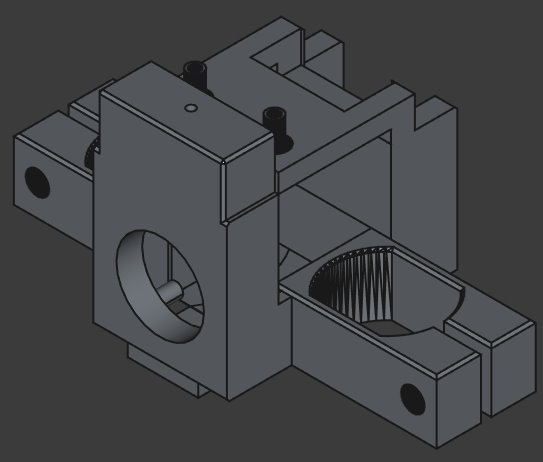
\includegraphics[width=\textwidth]{images/cad_gunarm_v2_front.jpg}
        \caption{Geschützarm Version 2 - Frontansicht}
    \end{subfigure}
    \hfill
    \begin{subfigure}[b]{0.45\textwidth}
        \centering
        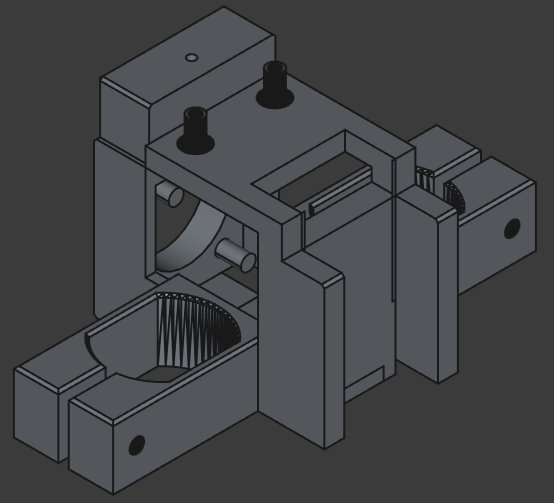
\includegraphics[width=\textwidth]{images/cad_gunarm_v2_back.jpg}
        \caption{Geschützarm Version 2 - Rückansicht}
    \end{subfigure}

    \caption{Geschützarm Version 2}
    \label{fig:gunarm_v2}
\end{figure}

Im Gegensatz zur Version 1 wird der Ultraschallsensor nun seitlich eingeführt anstatt von unten, siehe~\ref{fig:gunarm_v2}. Problematisch waren dabei die beschränkten Platzverhältnisse, da die Schrittmotoren näher am Kanonenrohr angebracht wurden als im vorherigen Entwurf. Außerdem wurden die zuvor angedachten Montagepunkte am Magazin wieder entfernt. Die Zusammenführung des Geschützarms mit dem Magazin erfolgte deshalb mittels Modellbaukleber.

\section{Montagehalterung Motortreiber (Specht)}

Für die ersten Funktionstests wurden die Pololu-Motoren provisorisch auf Kork-Schnipseln montiert. Dieses Vorgehen ermöglichte eine zügige Inbetriebnahme, jedoch erwies es sich hinsichtlich Stabilität und Sicherheit als unzureichend. Im Rahmen der Tests kam es zum Abrutschen eines Motors von der Korkunterlage, was zu einer kurzfristigen Wärmeentwicklung und Geruchsbildung führte. Glücklicherweise wurde eine Beschädigung der Hardware vermieden.

\begin{figure}[h]
    \centering

    \begin{subfigure}[b]{0.25\textwidth}
        \centering
        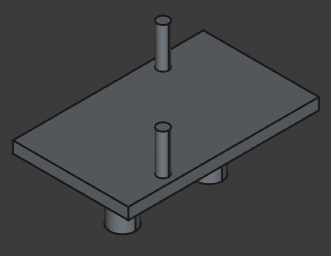
\includegraphics[width=\textwidth]{images/cad_polulu_front.png}
        \caption{Polulu - Draufsicht}
    \end{subfigure}
    \hspace{0.05\textwidth} % Adjust this value as needed
    \begin{subfigure}[b]{0.25\textwidth}
        \centering
        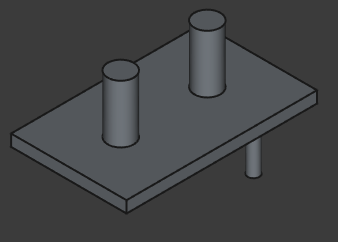
\includegraphics[width=\textwidth]{images/cad_polulu_back.png}
        \caption{Polulu - Bodensicht}
    \end{subfigure}

    \caption{Montagehalterung für Pololu-Motortreiber}
    \label{fig:pololu_mounting}
\end{figure}

Für die finale Abnahme wurde daher ein dauerhaftes und sicheres Montagesystem umgesetzt, das ein sauberes und zuverlässiges Setup gewährleistet. Wie in Abbildung~\ref{fig:pololu_mounting} zu sehen, kann die Halterung direkt auf der Montageplatte des Fahrzeugs geklippt werden.

\section{Dualshock4 Treiber (Becker)}

Gemäß der Anforderung ist die Steuerung des Fahrzeugs sowie der Geschützplattform durch einen DualShock4-Controller vorgesehen. 
Einerseits dient dies dem Testen der Plattformsteuerung für den späteren Betrieb der KI. 
Des Weiteren fungiert sie als Gamification-Element. 
Das Ziel ist die Steigerung des Nutzens und der Freude an dem Projekt, indem eine bekannte Steuerungsmethode verwendet wird, welche die Benutzerfreundlichkeit erhöht.

Für die Realisierung dieser Funktionalität wurde ein spezieller Treiber entwickelt, der den Zustand des Controllers in regelmäßigen Abständen an den ESP-32 übermittelt. 
Darüber hinaus umfasste mein Wunsch eine Funktion, die Vibrationen und Farbwechsel am Gamepad auslöst, und zwar vom Mikrocontroller aus.

\subsection{Übertragung}

Vor jeglicher Datenübertragung muss zunächst eine Kopplung per Bluetooth hergestellt werden. 
Der Sony Dualshock 4 Controller verwendet in diesem Fall den Bluetooth Classic 4.0 Standard.
Für die Verbindung des Controllers mit den Geräten ist im Flash-Speicher des Gamepads eine MAC-Adresse gespeichert. 
Beim Anschalten des Controllers wird versucht, Kontakt zu dieser Adresse aufzubauen.
Unter normalen Betriebsbedingungen wäre dies die Adresse der PlayStation4-Konsole. 
Für unser Projekt wurde jedoch die gespeicherte MAC-Adresse mit der des ESP-32 überschrieben.
Nach dem Einschalten unternimmt das Gamepad sofort den Versuch, sich mit dem Mikrocontroller zu verbinden.

Die Übertragung der Daten zwischen Gamepad und Mikrocontroller erfolgt mittels sogenannter HID-Reports.
HID-Reports sind binäre Datenstrukturen, welche die Reihenfolge der Informationen festlegen.
Die Struktur der Reports wurde von Sony nicht öffentlich zur Verfügung gestellt. 
Allerdings war es einigen Personen möglich, durch Reverse-Engineering wichtige Felder zu ermitteln \cite{esp_ds4_hid_reports}.

Das Human Interface Device (HID)-Protokoll ist ein standardisiertes Kommunikationsprotokoll zur Übertragung von Eingabe- und Steuerdaten zwischen Peripheriegeräten (z.B. Tastaturen, Mäusen, Gamepads) und einem Host-System. 
Es wurde ursprünglich für USB spezifiziert \cite{esp_usb_hid_spec} und später für Bluetooth Classic übernommen.

\begin{figure}[ht]
    \centering
    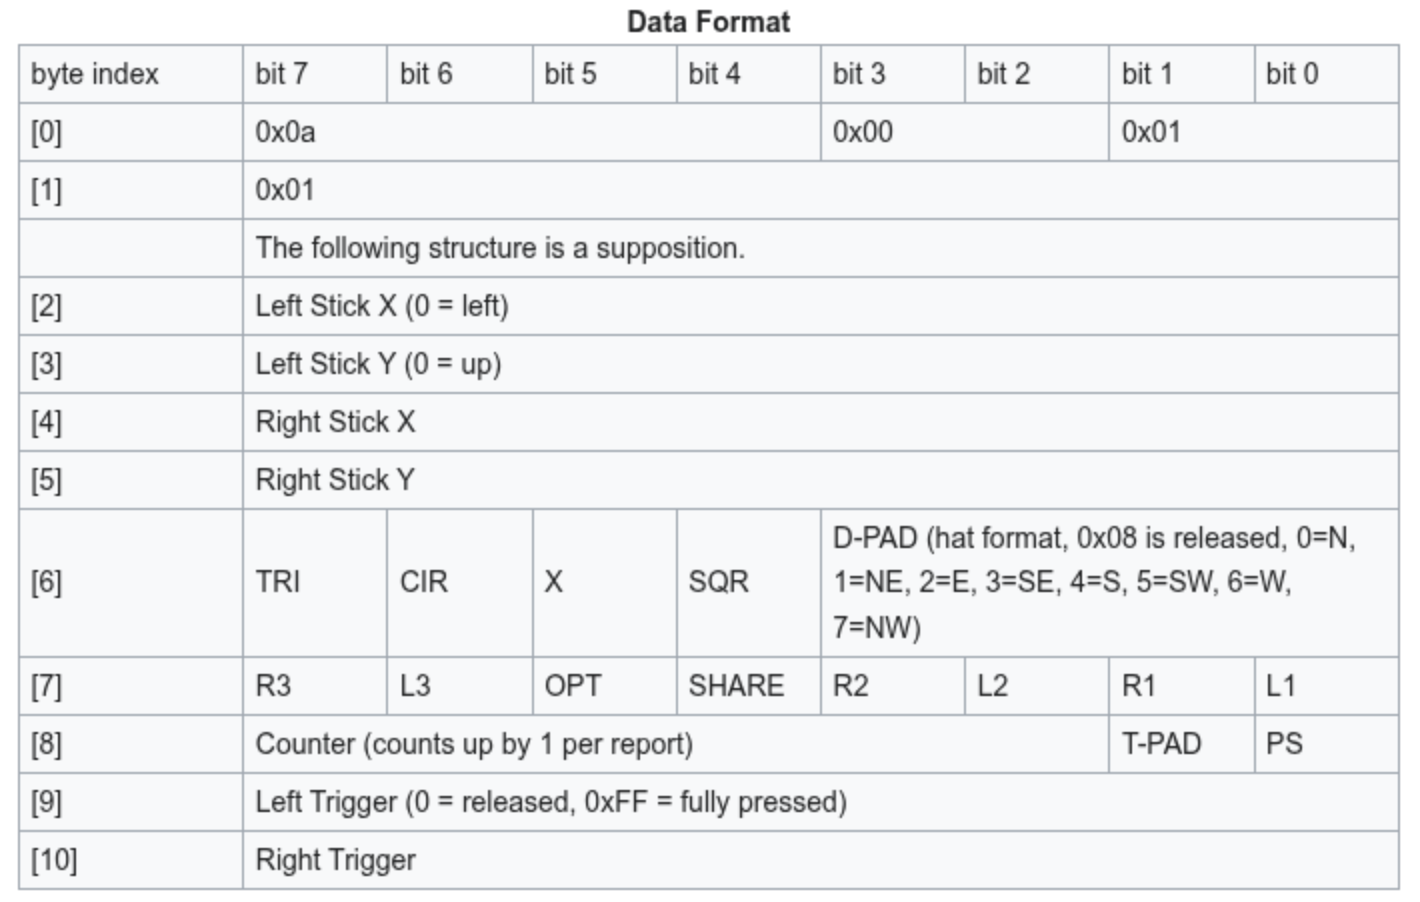
\includegraphics[width=0.7\textwidth]{images/becker_esp32_ds4_report.png}
    \caption{Beispielhafter Aufbau eines HID-Reports aus \cite{esp_ds4_hid_reports}}
\end{figure}

\subsection{Version 1: eigens entwickelter Treiber}

Eine Websuche nach existierenden DualShock-4-Treibern für das ESP-IDF brachte zunächst nur veraltete Implementierungen zutage, die auf nicht mehr unterstützten APIs basierten. 
Zahlreiche andere Ansätze zielten ausschließlich auf das Arduino-Framework ab und ließen sich daher nur eingeschränkt oder gar nicht in ein ESP-IDF-basiertes Projekt integrieren.

Da die Struktur der vom Gamepad gesendeten HID-Reports dank Reverse Engineering bekannt war und das ESP-IDF über eine Bluetooth-HID-Host-API verfügte \cite{esp_hib_bt_api}, wurde im ersten Ansatz ein eigener Treiber entwickelt.

Der Verbindungsaufbau verlief problemlos, und zu Beginn wurden die Input-Reports korrekt empfangen. 
Nach kurzer Zeit fror die Datenübertragung jedoch ein, obwohl alle anderen Tasks auf dem System weiterhin fehlerfrei ausgeführt wurden. 
Recherchen ergaben, dass dieses Verhalten auch von anderen Nutzern beobachtet wurde \cite{esp_hib_bt_api_issues}. 
Als Ursache wird die vergleichsweise hohe Sendefrequenz des Controllers vermutet, die laut Nutzertests bei über 700 Hz liegt \cite{esp_ds4_hid_reports}.

Um den Overhead in der Callback-Funktion für empfangene Reports zu reduzieren, wurde ein Zeitfilter implementiert. 
Ein Timer prüft beim Eintreffen eines Reports, ob seit dem letzten verarbeiteten Report mindestens $16.\overline{6}$ ms (entsprechend 60 Hz) vergangen sind. 
Ist dies der Fall, wird der aktuelle Report in eine durch FreeRTOS bereitgestellte Queue eingereiht. 
Diese wird von einem separaten Task abgearbeitet, der die Reports auf der Konsole protokolliert. 
Auf diese Weise konnte das Logging, das potenziell blockierend wirkt, vom zeitkritischen Pfad entkoppelt werden.

Obwohl diese Maßnahme die Zeitspanne, in der die Daten stabil übertragen wurden, verlängerte, wurde das zugrundeliegende Problem damit nicht vollständig gelöst. 
Nach einigen Minuten unterbrach der Controller die Übertragung der Reports erneut, obwohl die Status-LED weiterhin eine aktive Bluetooth-Verbindung anzeigte.

Da der ESP-32 in dieser Anwendung zusätzlich weitere zeitkritische Komponenten wie den Motortreiber verwalten muss, ist die Stabilität und Effizienz des Treibers von zentraler Bedeutung.
Aus diesem Grund wurde entschieden, die Entwicklung eines eigenen Treibers nicht weiter zu verfolgen und stattdessen nach einer robusteren und getesteten Alternative zu suchen.

\subsection{Version 2: Treiber basierend auf der Bluepad32 Bibliothek}

\subsection{Testing}

Um den funktionierenden Treiber zu testen wurden zwei Tasks auf dem ESP-32 erstellt:

\begin{itemize}
    \item \textbf{Input-Test Task}: Dieser Task wartet vor jedem Schleifendurchlauf auf verbinden, das bedeutet er ist so lange blockiert, bis der Dualshock-Controller die Verbindung hergestellt hat.
    Dann wartet er an der Input Queue bis der Controller einen Zustandsreport schickt. Dieser wir dann aus der Queue entnommen und auf der Konsole ausgegeben. Zuletzt wird $16.\overline{6}$ ms (60 Hz) gewartet.
    \item \textbf{Output-Test Task}: Hier wird ebenfalls blockiert bis das Gamepad verbunden ist. Nach dem die Verbindung aufgebaut ist wird je ein Vibrations- und Farbwechselevent in die Queue gelegt. 
    Da dass Vibrationsevent eine Dauer von 100 ms bekommen hat wird hier 100 ms gewartet.
\end{itemize}

Mit diesem simplen Testsetup konnten alle Funktionen des Controller getestet werden. 
Auch das Fortfahren nach einem Verbindungsabbruch konnten durch Aus- und Einschalten des Gamepads getestet werden. 

Bei Testen fiel weiterhin auf, dass die Batteriestandswarnung dauerhaft ausgelöst war, ein Blick auf die Input Werte zeigte, dass der Controller eine komplette leere Batterie anzeigte. 
Auch nach dem Aufladen fielen die Werte schnell wieder auf 0, obwohl am PC ganz andere Ladestände angezeigt wurden. (WIP!)

\section{Platformsteuerung (Becker)}

Die sogenannte Plattformsteuerung bezeichnet alle technischen Komponenten, die erforderlich sind, um die Plattform in ihrer Rotation, vertikalen Neigung sowie für die Abgabe eines Schusses zu steuern.

Für den genannten Zweck werden folgende Komponenten benötigt:

\begin{itemize}
    \item \textbf{Drehung und Neigung}
    \begin{itemize}
        \item zwei MG996R Servo Motoren
    \end{itemize}
    \item \textbf{Schussabgabe}
    \begin{itemize}
        \item zwei DC-Motoren (Flywheels)
        \item MG92B Servo Motor
    \end{itemize}
\end{itemize}

Da die maximale Ausgangsstärke eines GPIO-PINs des ESP-32 mit 40mA \cite[S.~53]{esp_datasheet} für die benötigten Motoren nicht ausreicht \cite{esp_platform_flywheel_motor,esp_platform_small_servo,esp_platform_servo}, wurden entsprechende Treiberbaords verwendet.
Konkret handelt es sich hierbei um ein PCA9685 PWM-Treiberboard für die Servomotoren und um per PWM steuerbare MOSFET-Module für die Flywheel-Motoren.

In der nachfolgenden Sektion wird der Entwurf des Codes erörtert, der erforderlich ist, um die genannten Teile anzusteuern.

\subsection{PWM Board Treiber (Becker)}

Das PCA9685 PWM-Treiberboard gestattet die gleichzeitige Anbindung von bis zu 16 Servomotoren.
Für die Stromversorgung steht ein Eingang mit einer Spannung von 5 Volt zur Verfügung.

Die Steuerung des Boards erfolgt durch das Schreiben verschiedener Werte in Konfigurationsregister, wobei das I²C-Protokoll zum Einsatz kommt. 
Der vorliegende Treiber wurde aus der Portierung eines bereits bestehenden Treibers \cite{esp_pca9685_blueprint} entwickelt, welcher in der Programmiersprache C++ implementiert war. 
Es wurde bewusst nur die Funktionalität portiert, die für den Umfang des Projekts von Relevanz war. 
Der Treiber umfasst demzufolge lediglich drei Funktionen:

\begin{itemize}
    \item \textbf{pca9685\_init}: Die Funktion erhält die gewünschte Konfiguration für das Board (beispielsweise die Bus-Adresse, die SDA- und SCL-Ports für den I²C-Bus) und initialisiert den I²C-Bus. 
    Im Anschluss registriert sie das Treiberboard und konfiguriert schließlich das Board mit der gewünschten PWM-Frequenz.
    \item \textbf{pca9685\_set\_pwm\_on\_off}: Mithilfe dieser Funktion besteht nun die Möglichkeit, einen Motor auf einem der 16 Kanäle zu steuern. 
    Der Parameter \textit{ON} ist eine 12-Bit Zahl beschreibt hierbei den Zeitpunkt in der Phase, an welchem der Ausgang auf 5 Volt geschalten wird. 
    \textit{OFF}, ebenfalls eine 12-Bit Zahl bezeichnet den Zeitpunkt, zu welchem der Ausgang wieder auf 0 Volt geregelt wird. 
    Eine grafische Veranschaulichung ist in Abbildung \ref{fig:esp_pca9685_on_off} ersichtlich. 
    Da für die Ansteuerung der Servo Motoren keine symmetrischen PWM-Signale benötigt werden, wird der Parameter \textit{ON} im Folgenden immer den Wert 0 annehmen.

    \begin{figure}[ht]
        \centering
        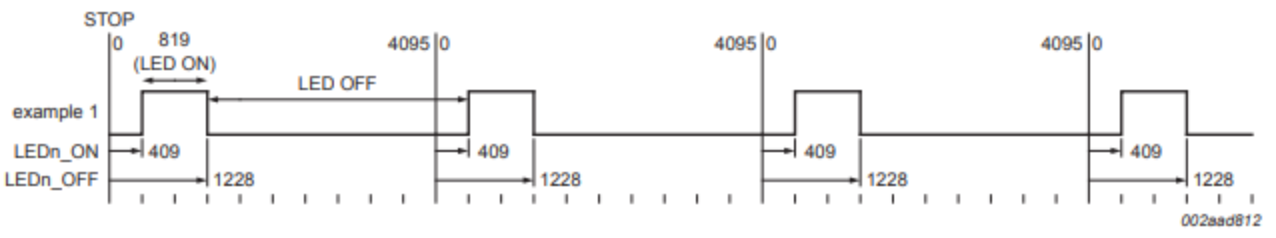
\includegraphics[width=\textwidth]{images/becker_esp_pca9685.png}
        \caption{Erklärung ON\slash OFF Parameter für PCA9685 aus \cite[S.~17]{esp_pca9685_datasheet}}
        \label{fig:esp_pca9685_on_off}
    \end{figure}

    \item \textbf{pca9685\_set\_off}: Mittels dieser Funktion kann das PWM-Signal auf einem bestimmten Kanal deaktiviert werden.
\end{itemize}

Auf Basis dieses Treiber wurden im nächsten Schritt zwei Interfaces programmiert: 
Einerseits das Interface zur Plattform-Kontrolle und andererseits das Interface zur Schusskontrolle, welches zusätzlich der Logik zur Ansteuerung der Flywheel-Motoren enthält.

\subsection{Ansteuerung der Servo-Motoren (Becker)}

Um nun die Plattform sowohl manuell über den DualShock4-Controller als auch semi-automatisch per künstlicher Intelligenz über MQTT präzise steuern zu können, wurde ein Interface entwickelt, das die Ansteuerung eines Motors an eine bestimmte Position erlaubt. 

In diesem Kontext wird mit der Einheit Grad gearbeitet. 
Ein Blick in die Referenz \cite{esp_servo_control} der Servo-Motoren zeigt, dass durch die Einstellung der Duty-Cycle-Länge des PWM-Signals eine Drehung auf eine bestimmte Grad-Position erreicht wird. 
Im ersten Schritt wurden die \textit{OFF} Werte für die Punkte \ang{-90} (max. Drehung nach links), \ang{0} und \ang{90} (max. Drehung nach rechts) manuell ermittelt.
Die absoluten Werte für die Drehungen werden im Folgenden als $value_{-90^\circ}$, $value_{0^\circ}$ und $value_{90^\circ}$ bezeichnet.

Für die Berechnung des Zielwerts $value_{off}$ für den \textit{OFF} Wert des PWM-Board-Treibers aus einem gegebenen Winkel wird Formel \ref{eq:pwm_to_duty} verwendet.

\begin{gather}
    \begin{aligned}
    &\text{Sei } \theta \text{ der gewünschte Winkel,} \\
    &|\theta| = \text{Betrag von } \theta \\
    &n_3 = \left\lfloor \frac{|\theta|}{3} \right\rfloor \\
    &n_2 = |\theta| - n_3 \\
    &s = 2 \cdot n_2 + 3 \cdot n_3 \\
    &\tilde{s} =
    \begin{cases}
    s, & \theta > 0 \\
    -s, & \theta \leq 0
    \end{cases} \\
    &value_{off} = value_{zero} + \tilde{s}
    \end{aligned}
    \label{eq:pwm_to_duty}
\end{gather}

Die Idee der Formel beruht auf der Tatsache, dass die Differenz aus $value_{90^\circ}$ bzw. $value_{-90^\circ}$ und $value_{0^\circ}$ gebildet und anschließend gleichmäßig auf den Bereich von $]1, 90[$, also auf 90 Werte, aufgeteilt wird. 

Für jedes zusätzliche Grad Rotation um den Nullpunkt müssten demnach entweder $2.\overline{3}$ addiert oder subtrahiert werden.
Da dies in Anbetracht der Verwendung von Festkommazahlen nicht realisierbar wäre, erscheint die naheliegende Idee, den Wert zu runden. 
Diese Praktik würde jedoch im Zeitverlauf zu einer zunehmenden Abweichung und folglich zu einem Verlust an Präzision führen.
Um das genannte Problem zu vermeiden, wird der \textit{OFF} Wert für jedes dritte Grad Drehung um den Faktor 3 verändert und für jedes andere Grad um Faktor 2.
Die Formel \ref{eq:pwm_to_duty} berechnet dabei in $n_3$ die Anzahl der Faktor-3-Drehungen und in $n_2$ die Anzahl der Faktor-2-Drehungen.
Ausgehend davon wird $value_{0^\circ}$ verändert.

Das Endergebnis stellt eine Funktion dar, mittels derer eine präzise gradweise Ansteuerung beider Plattformachsen möglich ist.

Darüber hinaus wurde im Interface ein Clipping der Werte als Sicherheitmechanismus integriert. Im Zuge der Initialisierung des Plattforminterfaces muss für jede Achse ein Startwinkel sowie ein linker und rechter Stopwinkel angegeben werden.
Sollte es bei der Steuerung durch den Dualshock4-Controller in dessen Regelschleife oder in der KI-Berechnung zu einem fehlerhaften Gradwert kommen, wird dieser Wert automatisch an den nächstgelegenen Stopwinkel geclippt. 
Durch diese Maßnahme werden potenzielle Materialschäden, die durch fehlerhafte Drehungen verursacht werden könnten, verhindert.

Die Realisierung der Ansteuerung des kleinen Servos, dessen Funktion darin besteht, die Nerf-Darts in die Flywheel-Motoren zu schieben, würde durch die Verwendung dieser Art der Ansteuerung zu einer unnötigen Komplexität führen.
Daher wurde für diesen Motor lediglich eine Startposition (Geschütztrigger ganz hinten; Dart kann in das Magazin fallen) und eine Endposition (Geschütztrigger ganz vorne; Dart wurde in die Flywheels geschoben) durch manuelles Einsetzen von \textit{OFF} Werten festgelegt.
Wird nun ein Schuss ausgelöst, so fährt der Servo-Motor zunächst in seine Endposition und von dort aus wieder zurück in seine Startposition.

\subsection{Ansteuerung der Flywheel Motoren (Becker, Koch, Wohlrab)}

Für die Vervollständigung des Fire-Control Interfaces wird nun noch die Ansteuerung der Flywheel-Motoren benötigt.
In dem vorliegenden Projekt erfolgt die Steuerung der beiden Gleichstrommotoren jeweils durch ein Power-MOSFET-Modul.

Die Funktionsweise des Modul lässt sich folgendermaßen beschreiben:

\begin{itemize}
    \item Auf einer Seite wird der Eingangstrom, in unserem Fall 5V, vom Stromverteiler eingeführt.
    \item Andererseits wird der Ausgang jeweils mit einem Motor verbunden.
    \item Die am Ausgang ausgegebene Spannung kann über einen PWM-Pin geregelt werden \cite{esp_platform_flywheel_motor}.
\end{itemize}

Die Wahl fiel auf dieses relativ simple Modul, da lediglich die Anforderung bestand, dass sich die Motoren bei der Schussabgabe möglichst schnell drehen sollen.
Im Rahmen dieses Projekts waren keine Änderungen der Richtung oder präzisere Steuerung erforderlich.

Im Rahmen des manuellen Tests wurde festgestellt, dass zur Erzielung eines optimalen Schussbildes eine Versorgung der Motoren mit 5 Volt erforderlich ist. 
Infolgedessen beträgt der Duty-Cycle entweder 0 oder 100 Prozent.
Daher wurde der ursprüngliche PWM-Code letztlich auf das reine Ein- und Ausschalten eines GPIO-Pins reduziert.

\section{Integration (Becker, Specht)}
\section{Dualshock4 Treiber (Becker)}

Gemäß der Anforderung ist die Steuerung des Fahrzeugs sowie der Geschützplattform durch einen DualShock4-Controller vorgesehen. 
Einerseits dient dies dem Testen der Plattformsteuerung für den späteren Betrieb der KI. 
Des Weiteren fungiert sie als Gamification-Element. 
Das Ziel ist die Steigerung des Nutzens und der Freude an dem Projekt, indem eine bekannte Steuerungsmethode verwendet wird, welche die Benutzerfreundlichkeit erhöht.

Für die Realisierung dieser Funktionalität wurde ein spezieller Treiber entwickelt, der den Zustand des Controllers in regelmäßigen Abständen an den ESP-32 übermittelt. 
Darüber hinaus umfasste mein Wunsch eine Funktion, die Vibrationen und Farbwechsel am Gamepad auslöst, und zwar vom Mikrocontroller aus.

\subsection{Übertragung}

Vor jeglicher Datenübertragung muss zunächst eine Kopplung per Bluetooth hergestellt werden. 
Der Sony Dualshock 4 Controller verwendet in diesem Fall den Bluetooth Classic 4.0 Standard.
Für die Verbindung des Controllers mit den Geräten ist im Flash-Speicher des Gamepads eine MAC-Adresse gespeichert. 
Beim Anschalten des Controllers wird versucht, Kontakt zu dieser Adresse aufzubauen.
Unter normalen Betriebsbedingungen wäre dies die Adresse der PlayStation4-Konsole. 
Für unser Projekt wurde jedoch die gespeicherte MAC-Adresse mit der des ESP-32 überschrieben.
Nach dem Einschalten unternimmt das Gamepad sofort den Versuch, sich mit dem Mikrocontroller zu verbinden.

Die Übertragung der Daten zwischen Gamepad und Mikrocontroller erfolgt mittels sogenannter HID-Reports.
HID-Reports sind binäre Datenstrukturen, welche die Reihenfolge der Informationen festlegen.
Die Struktur der Reports wurde von Sony nicht öffentlich zur Verfügung gestellt. 
Allerdings war es einigen Personen möglich, durch Reverse-Engineering wichtige Felder zu ermitteln \cite{esp_ds4_hid_reports}.

Das Human Interface Device (HID)-Protokoll ist ein standardisiertes Kommunikationsprotokoll zur Übertragung von Eingabe- und Steuerdaten zwischen Peripheriegeräten (z.B. Tastaturen, Mäusen, Gamepads) und einem Host-System. 
Es wurde ursprünglich für USB spezifiziert \cite{esp_usb_hid_spec} und später für Bluetooth Classic übernommen.

\begin{figure}[ht]
    \centering
    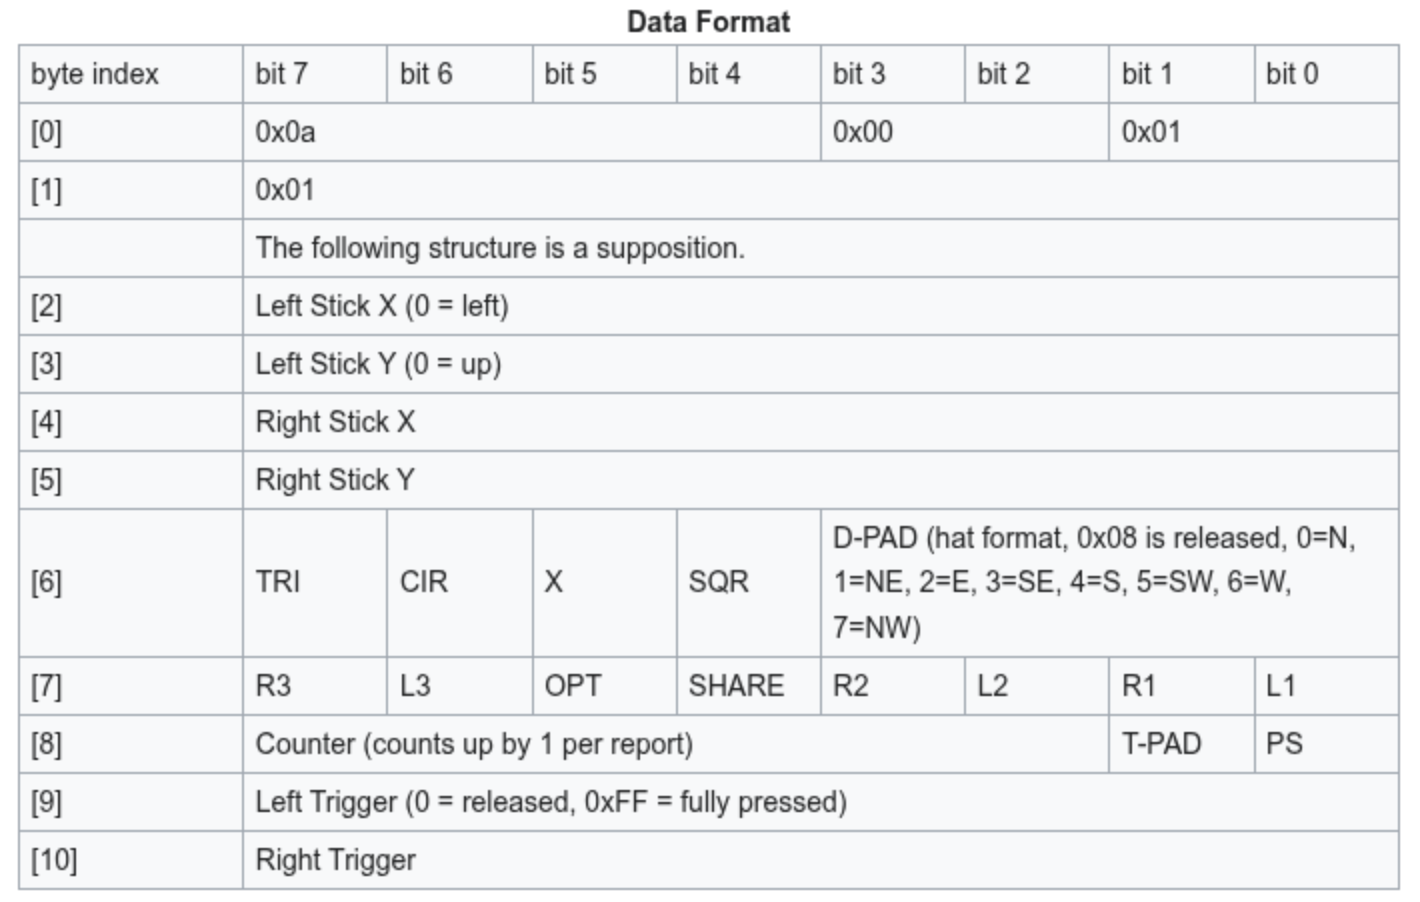
\includegraphics[width=0.7\textwidth]{images/becker_esp32_ds4_report.png}
    \caption{Beispielhafter Aufbau eines HID-Reports aus \cite{esp_ds4_hid_reports}}
\end{figure}

\subsection{Version 1: eigens entwickelter Treiber}

Eine Websuche nach existierenden DualShock-4-Treibern für das ESP-IDF brachte zunächst nur veraltete Implementierungen zutage, die auf nicht mehr unterstützten APIs basierten. 
Zahlreiche andere Ansätze zielten ausschließlich auf das Arduino-Framework ab und ließen sich daher nur eingeschränkt oder gar nicht in ein ESP-IDF-basiertes Projekt integrieren.

Da die Struktur der vom Gamepad gesendeten HID-Reports dank Reverse Engineering bekannt war und das ESP-IDF über eine Bluetooth-HID-Host-API verfügte \cite{esp_hib_bt_api}, wurde im ersten Ansatz ein eigener Treiber entwickelt.

Der Verbindungsaufbau verlief problemlos, und zu Beginn wurden die Input-Reports korrekt empfangen. 
Nach kurzer Zeit fror die Datenübertragung jedoch ein, obwohl alle anderen Tasks auf dem System weiterhin fehlerfrei ausgeführt wurden. 
Recherchen ergaben, dass dieses Verhalten auch von anderen Nutzern beobachtet wurde \cite{esp_hib_bt_api_issues}. 
Als Ursache wird die vergleichsweise hohe Sendefrequenz des Controllers vermutet, die laut Nutzertests bei über 700 Hz liegt \cite{esp_ds4_hid_reports}.

Um den Overhead in der Callback-Funktion für empfangene Reports zu reduzieren, wurde ein Zeitfilter implementiert. 
Ein Timer prüft beim Eintreffen eines Reports, ob seit dem letzten verarbeiteten Report mindestens $16.\overline{6}$ ms (entsprechend 60 Hz) vergangen sind. 
Ist dies der Fall, wird der aktuelle Report in eine durch FreeRTOS bereitgestellte Queue eingereiht. 
Diese wird von einem separaten Task abgearbeitet, der die Reports auf der Konsole protokolliert. 
Auf diese Weise konnte das Logging, das potenziell blockierend wirkt, vom zeitkritischen Pfad entkoppelt werden.

Obwohl diese Maßnahme die Zeitspanne, in der die Daten stabil übertragen wurden, verlängerte, wurde das zugrundeliegende Problem damit nicht vollständig gelöst. 
Nach einigen Minuten unterbrach der Controller die Übertragung der Reports erneut, obwohl die Status-LED weiterhin eine aktive Bluetooth-Verbindung anzeigte.

Da der ESP-32 in dieser Anwendung zusätzlich weitere zeitkritische Komponenten wie den Motortreiber verwalten muss, ist die Stabilität und Effizienz des Treibers von zentraler Bedeutung.
Aus diesem Grund wurde entschieden, die Entwicklung eines eigenen Treibers nicht weiter zu verfolgen und stattdessen nach einer robusteren und getesteten Alternative zu suchen.

\subsection{Version 2: Treiber basierend auf der Bluepad32 Bibliothek}

\subsection{Testing}

Um den funktionierenden Treiber zu testen wurden zwei Tasks auf dem ESP-32 erstellt:

\begin{itemize}
    \item \textbf{Input-Test Task}: Dieser Task wartet vor jedem Schleifendurchlauf auf verbinden, das bedeutet er ist so lange blockiert, bis der Dualshock-Controller die Verbindung hergestellt hat.
    Dann wartet er an der Input Queue bis der Controller einen Zustandsreport schickt. Dieser wir dann aus der Queue entnommen und auf der Konsole ausgegeben. Zuletzt wird $16.\overline{6}$ ms (60 Hz) gewartet.
    \item \textbf{Output-Test Task}: Hier wird ebenfalls blockiert bis das Gamepad verbunden ist. Nach dem die Verbindung aufgebaut ist wird je ein Vibrations- und Farbwechselevent in die Queue gelegt. 
    Da dass Vibrationsevent eine Dauer von 100 ms bekommen hat wird hier 100 ms gewartet.
\end{itemize}

Mit diesem simplen Testsetup konnten alle Funktionen des Controller getestet werden. 
Auch das Fortfahren nach einem Verbindungsabbruch konnten durch Aus- und Einschalten des Gamepads getestet werden. 

Bei Testen fiel weiterhin auf, dass die Batteriestandswarnung dauerhaft ausgelöst war, ein Blick auf die Input Werte zeigte, dass der Controller eine komplette leere Batterie anzeigte. 
Auch nach dem Aufladen fielen die Werte schnell wieder auf 0, obwohl am PC ganz andere Ladestände angezeigt wurden. (WIP!)

\section{Platformsteuerung (Becker)}

Die sogenannte Plattformsteuerung bezeichnet alle technischen Komponenten, die erforderlich sind, um die Plattform in ihrer Rotation, vertikalen Neigung sowie für die Abgabe eines Schusses zu steuern.

Für den genannten Zweck werden folgende Komponenten benötigt:

\begin{itemize}
    \item \textbf{Drehung und Neigung}
    \begin{itemize}
        \item zwei MG996R Servo Motoren
    \end{itemize}
    \item \textbf{Schussabgabe}
    \begin{itemize}
        \item zwei DC-Motoren (Flywheels)
        \item MG92B Servo Motor
    \end{itemize}
\end{itemize}

Da die maximale Ausgangsstärke eines GPIO-PINs des ESP-32 mit 40mA \cite[S.~53]{esp_datasheet} für die benötigten Motoren nicht ausreicht \cite{esp_platform_flywheel_motor,esp_platform_small_servo,esp_platform_servo}, wurden entsprechende Treiberbaords verwendet.
Konkret handelt es sich hierbei um ein PCA9685 PWM-Treiberboard für die Servomotoren und um per PWM steuerbare MOSFET-Module für die Flywheel-Motoren.

In der nachfolgenden Sektion wird der Entwurf des Codes erörtert, der erforderlich ist, um die genannten Teile anzusteuern.

\subsection{PWM Board Treiber (Becker)}

Das PCA9685 PWM-Treiberboard gestattet die gleichzeitige Anbindung von bis zu 16 Servomotoren.
Für die Stromversorgung steht ein Eingang mit einer Spannung von 5 Volt zur Verfügung.

Die Steuerung des Boards erfolgt durch das Schreiben verschiedener Werte in Konfigurationsregister, wobei das I²C-Protokoll zum Einsatz kommt. 
Der vorliegende Treiber wurde aus der Portierung eines bereits bestehenden Treibers \cite{esp_pca9685_blueprint} entwickelt, welcher in der Programmiersprache C++ implementiert war. 
Es wurde bewusst nur die Funktionalität portiert, die für den Umfang des Projekts von Relevanz war. 
Der Treiber umfasst demzufolge lediglich drei Funktionen:

\begin{itemize}
    \item \textbf{pca9685\_init}: Die Funktion erhält die gewünschte Konfiguration für das Board (beispielsweise die Bus-Adresse, die SDA- und SCL-Ports für den I²C-Bus) und initialisiert den I²C-Bus. 
    Im Anschluss registriert sie das Treiberboard und konfiguriert schließlich das Board mit der gewünschten PWM-Frequenz.
    \item \textbf{pca9685\_set\_pwm\_on\_off}: Mithilfe dieser Funktion besteht nun die Möglichkeit, einen Motor auf einem der 16 Kanäle zu steuern. 
    Der Parameter \textit{ON} ist eine 12-Bit Zahl beschreibt hierbei den Zeitpunkt in der Phase, an welchem der Ausgang auf 5 Volt geschalten wird. 
    \textit{OFF}, ebenfalls eine 12-Bit Zahl bezeichnet den Zeitpunkt, zu welchem der Ausgang wieder auf 0 Volt geregelt wird. 
    Eine grafische Veranschaulichung ist in Abbildung \ref{fig:esp_pca9685_on_off} ersichtlich. 
    Da für die Ansteuerung der Servo Motoren keine symmetrischen PWM-Signale benötigt werden, wird der Parameter \textit{ON} im Folgenden immer den Wert 0 annehmen.

    \begin{figure}[ht]
        \centering
        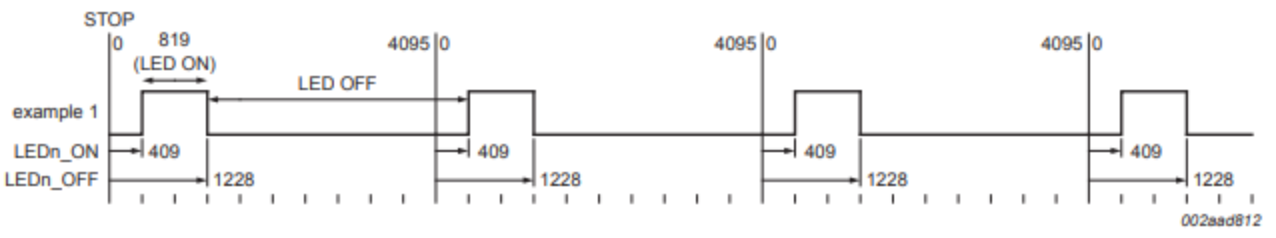
\includegraphics[width=\textwidth]{images/becker_esp_pca9685.png}
        \caption{Erklärung ON\slash OFF Parameter für PCA9685 aus \cite[S.~17]{esp_pca9685_datasheet}}
        \label{fig:esp_pca9685_on_off}
    \end{figure}

    \item \textbf{pca9685\_set\_off}: Mittels dieser Funktion kann das PWM-Signal auf einem bestimmten Kanal deaktiviert werden.
\end{itemize}

Auf Basis dieses Treiber wurden im nächsten Schritt zwei Interfaces programmiert: 
Einerseits das Interface zur Plattform-Kontrolle und andererseits das Interface zur Schusskontrolle, welches zusätzlich der Logik zur Ansteuerung der Flywheel-Motoren enthält.

\subsection{Ansteuerung der Servo-Motoren (Becker)}

Um nun die Plattform sowohl manuell über den DualShock4-Controller als auch semi-automatisch per künstlicher Intelligenz über MQTT präzise steuern zu können, wurde ein Interface entwickelt, das die Ansteuerung eines Motors an eine bestimmte Position erlaubt. 

In diesem Kontext wird mit der Einheit Grad gearbeitet. 
Ein Blick in die Referenz \cite{esp_servo_control} der Servo-Motoren zeigt, dass durch die Einstellung der Duty-Cycle-Länge des PWM-Signals eine Drehung auf eine bestimmte Grad-Position erreicht wird. 
Im ersten Schritt wurden die \textit{OFF} Werte für die Punkte \ang{-90} (max. Drehung nach links), \ang{0} und \ang{90} (max. Drehung nach rechts) manuell ermittelt.
Die absoluten Werte für die Drehungen werden im Folgenden als $value_{-90^\circ}$, $value_{0^\circ}$ und $value_{90^\circ}$ bezeichnet.

Für die Berechnung des Zielwerts $value_{off}$ für den \textit{OFF} Wert des PWM-Board-Treibers aus einem gegebenen Winkel wird Formel \ref{eq:pwm_to_duty} verwendet.

\begin{gather}
    \begin{aligned}
    &\text{Sei } \theta \text{ der gewünschte Winkel,} \\
    &|\theta| = \text{Betrag von } \theta \\
    &n_3 = \left\lfloor \frac{|\theta|}{3} \right\rfloor \\
    &n_2 = |\theta| - n_3 \\
    &s = 2 \cdot n_2 + 3 \cdot n_3 \\
    &\tilde{s} =
    \begin{cases}
    s, & \theta > 0 \\
    -s, & \theta \leq 0
    \end{cases} \\
    &value_{off} = value_{zero} + \tilde{s}
    \end{aligned}
    \label{eq:pwm_to_duty}
\end{gather}

Die Idee der Formel beruht auf der Tatsache, dass die Differenz aus $value_{90^\circ}$ bzw. $value_{-90^\circ}$ und $value_{0^\circ}$ gebildet und anschließend gleichmäßig auf den Bereich von $]1, 90[$, also auf 90 Werte, aufgeteilt wird. 

Für jedes zusätzliche Grad Rotation um den Nullpunkt müssten demnach entweder $2.\overline{3}$ addiert oder subtrahiert werden.
Da dies in Anbetracht der Verwendung von Festkommazahlen nicht realisierbar wäre, erscheint die naheliegende Idee, den Wert zu runden. 
Diese Praktik würde jedoch im Zeitverlauf zu einer zunehmenden Abweichung und folglich zu einem Verlust an Präzision führen.
Um das genannte Problem zu vermeiden, wird der \textit{OFF} Wert für jedes dritte Grad Drehung um den Faktor 3 verändert und für jedes andere Grad um Faktor 2.
Die Formel \ref{eq:pwm_to_duty} berechnet dabei in $n_3$ die Anzahl der Faktor-3-Drehungen und in $n_2$ die Anzahl der Faktor-2-Drehungen.
Ausgehend davon wird $value_{0^\circ}$ verändert.

Das Endergebnis stellt eine Funktion dar, mittels derer eine präzise gradweise Ansteuerung beider Plattformachsen möglich ist.

Darüber hinaus wurde im Interface ein Clipping der Werte als Sicherheitmechanismus integriert. Im Zuge der Initialisierung des Plattforminterfaces muss für jede Achse ein Startwinkel sowie ein linker und rechter Stopwinkel angegeben werden.
Sollte es bei der Steuerung durch den Dualshock4-Controller in dessen Regelschleife oder in der KI-Berechnung zu einem fehlerhaften Gradwert kommen, wird dieser Wert automatisch an den nächstgelegenen Stopwinkel geclippt. 
Durch diese Maßnahme werden potenzielle Materialschäden, die durch fehlerhafte Drehungen verursacht werden könnten, verhindert.

Die Realisierung der Ansteuerung des kleinen Servos, dessen Funktion darin besteht, die Nerf-Darts in die Flywheel-Motoren zu schieben, würde durch die Verwendung dieser Art der Ansteuerung zu einer unnötigen Komplexität führen.
Daher wurde für diesen Motor lediglich eine Startposition (Geschütztrigger ganz hinten; Dart kann in das Magazin fallen) und eine Endposition (Geschütztrigger ganz vorne; Dart wurde in die Flywheels geschoben) durch manuelles Einsetzen von \textit{OFF} Werten festgelegt.
Wird nun ein Schuss ausgelöst, so fährt der Servo-Motor zunächst in seine Endposition und von dort aus wieder zurück in seine Startposition.

\subsection{Ansteuerung der Flywheel Motoren (Becker, Koch, Wohlrab)}

Für die Vervollständigung des Fire-Control Interfaces wird nun noch die Ansteuerung der Flywheel-Motoren benötigt.
In dem vorliegenden Projekt erfolgt die Steuerung der beiden Gleichstrommotoren jeweils durch ein Power-MOSFET-Modul.

Die Funktionsweise des Modul lässt sich folgendermaßen beschreiben:

\begin{itemize}
    \item Auf einer Seite wird der Eingangstrom, in unserem Fall 5V, vom Stromverteiler eingeführt.
    \item Andererseits wird der Ausgang jeweils mit einem Motor verbunden.
    \item Die am Ausgang ausgegebene Spannung kann über einen PWM-Pin geregelt werden \cite{esp_platform_flywheel_motor}.
\end{itemize}

Die Wahl fiel auf dieses relativ simple Modul, da lediglich die Anforderung bestand, dass sich die Motoren bei der Schussabgabe möglichst schnell drehen sollen.
Im Rahmen dieses Projekts waren keine Änderungen der Richtung oder präzisere Steuerung erforderlich.

Im Rahmen des manuellen Tests wurde festgestellt, dass zur Erzielung eines optimalen Schussbildes eine Versorgung der Motoren mit 5 Volt erforderlich ist. 
Infolgedessen beträgt der Duty-Cycle entweder 0 oder 100 Prozent.
Daher wurde der ursprüngliche PWM-Code letztlich auf das reine Ein- und Ausschalten eines GPIO-Pins reduziert.

\section{Integration (Becker, Specht)}

\section{Gyrosensor Programmierung (Koch)}
Zu Beginn des Projekts war geplant den Gyrosensor MPU6050 zu nutzen, um die Position der Geschützplattform zu bestimmen, da eine kontinuierliche Bewegung um die eigene Achse aufgrund der Kabel nicht möglich ist. Dabei sollte der Sensor über den I2C-Bus mit dem Raspberry Pi 5 verbunden werden, um die Daten auszulesen und zu verarbeiten.
Der MPU6050 ist dabei ein 3-Achsen-Gyroskop und 3-Achsen-Beschleunigungssensor, welcher entsprechende Drehbewegungen und Beschleunigungen entlang der Raumachsen messen kann, welche für eine genaue Winkelbestimmung notwendig sind.

Nach kurzem Einlesen in die Dokumentation waren erste Rohdaten leicht auszulesen. Diese Rohdaten liegen in Form von 16 Bit in zwei Registern bereit und haben die Einheit $\mathit{LSB/g}$ für die Beschleunigungswerte und $\mathit{LSB/^\circ s}$ für die Gyroskop-Werte. Dies gilt es in tatsächliche physikalische Größen umzuwandeln, was bei unserem Projekt letztlich einem Winkel entspricht. 
Um die Beschleunigungswerte nutzen zu können, muss dafür mittels des Skalierungsfaktors die Fallbeschleunigung $\mathit{g}$ errechnet werden, indem man den erhaltenen Wert $x/16384$ rechnet. Die $16384$ ergeben sich aus der Dokumentation und entsprechen den LSB bei einem Messbereich von $\pm2g$, welches der Standardauflösung entspricht und auch die höchste Auflösung des MPU6050 für ist.
Ähnlich wird nun auch Winkelgeschwindigkeit ($\mathit{^\circ s}$) errechnet. Hierbei beträgt der Teiler standardmäßig $131$. \cite[S. 12-13]{raspberry_invensense_mpu6050_datasheet} 

Nach der Umrechnung der Rohdaten in physikalische Größen können nun die Neigungswinkel (Roll- und Pitch-Winkel) des Sensors berechnet werden. Diese ergeben sich aus der Richtung der Erdbeschleunigung relativ zum Sensor. 

Dazu wird die Erweiterung des Arkustangens genutzt, genauer gesagt die Funktion \texttt{atan2}, da sie im Gegensatz zum gewöhnlichen Arctangens auch die Orientierung in allen vier Quadranten berücksichtigt und somit stabile Winkelwerte über den gesamten Bereich von $-180^\circ$ bis $+180^\circ$ liefert. \cite{raspberry_matlab_atan2}

Die Winkelberechnung erfolgt nach der Formel \ref{eq:norms_to_angle}:

\begin{gather}
    \begin{aligned}
    \varphi_\text{pitch} &= \arctan2\left(a_y,\sqrt{a_x^2 + a_z^2}\right) \cdot \frac{180^\circ}{\pi} \\
    \varphi_\text{roll}  &= \arctan2\left(a_x,\sqrt{a_y^2 + a_z^2}\right) \cdot \frac{180^\circ}{\pi}
    \end{aligned}
    \label{eq:norms_to_angle}
\end{gather}


Hierbei sind $a_x$, $a_y$ und $a_z$ die normierten Beschleunigungswerte in $\mathit{g}$ (berechnet aus den Rohwerten durch Division durch $16384$). 

Die $atan2$-Funktion liefert den Winkel zwischen der positiven $x$-Achse und dem Punkt $(x, y)$ in der Ebene, wodurch Sprünge oder Mehrdeutigkeiten bei $90^\circ$ vermieden werden. \cite{raspberry_matlab_atan2}

Nachdem der Term im Code implementiert wurde, konnte ein starkes Rauschen beobachtet werden, was zunächst auf natürliche Schwankungen des Sensors zurückgeführt wurde, weshalb sich dazu entschieden wurde zuerst einen Komplementärfilter zu implementieren,
welcher allerdings das Problem nur bedingt beheben konnte. Deshalb wurde auch noch der Kalman-Filter ausgetestet, wodurch auch eine starke  Rauschunterdrückung festgestellt werden konnte, doch auch hier zeichnete sich ein überdurchschnittliches Rauschverhalten ab, weshalb der Fehler nicht mehr auf ein natürliches Rauschen zurückzuführen war.
Daraufhin wurde auch ein zweiter MPU6050 getestet, welcher ebenfalls dieses Verhalten aufwies, wodurch klar wurde, dass es sich hierbei um einen Programmierfehler handeln muss. Dieser konnte nach einiger Zeit auch herausgefunden werden und lag an der Interpretation der Rohdaten, 
welche fälschlicherweise als \texttt{int16\_t} statt \texttt{uint16\_t} interpretiert wurden.

Aufgrund der aufgewendeten Zeit für die Implementierung des Kalman-Filters sollte dieser aber trotzdem Anwendung im Projekt finden und wird in \ref{sec:kalman_filter} behandelt.

Wie Eingangs erwähnt, sollte der Gyrosensor MPU6050 genutzt werden, um die Position der Geschützplattform zu bestimmen, wofür der Winkel der Drehung um die eigene Achse benötigt wird. Dabei stellte sich heraus das der MPU6050 für diesen Wert zu einem starken Drift neigt, weshalb empfohlen wird diesen mit einem Magnetometer zu kombinieren \cite[S. 26]{raspberry_invensense_mpu6050_datasheet}.
Zur gleichen Zeit stellte sich heraus, dass diese Funktionalität nicht benötigt wird, da über die Servo-Motoren bereits ein Nullpunkt definiert werden konnte, weshalb der Gyrosensor letztlich nur noch für die Neigung der Geschützplattform genutzt wird, um diese als Debug-Information auf dem Webserver \ref{sec:Webserver} anzuzeigen.

\subsection{Kalman Filter Implementierung (Koch)}
\label{sec:kalman_filter}
Der Kalman-Filter ist ein Algorithmus zur Schätzung des Zustands eines dynamischen Systems. Er nutzt Messwerte mit einem mathematischen Modell, um aus verrauschten Daten optimale Schätzungen zu erzeugen und zu filtern, was insbesondere bei Sensoren mit Rauschen, wie dem MPU6050, von Bedeutung ist \cite{raspberry_rwth_kalman_2025}.
Die Berechnung des Kalman-Filters erfolgt nun mittels der Werte des Gyroskops, einer Zeitdifferenz und der zuvor berechneten Roll-und Pitchwinkel. Die Neigungswinkel liefern eine absolute Orientierung relativ zur Erdgravitation, sind jedoch anfällig gegenüber Rauschen und dynamischen Bewegungen, da sie auf Momentanwerten basieren, weshalb man hier auf die Gyroskopwerte zurückgreift.
Diese liefern die Winkelgeschwindigkeit, also die Änderungsrate der Orientierung. Diese Werte werden über die Zeit integriert, um eine relative Winkelschätzung zu erhalten. Sie zeichnen sich durch hohe Kurzzeitstabilität und geringe Reaktionsverzögerung aus, unterliegen jedoch einem Driftverhalten aufgrund von Messabweichungen und systematischen Fehlern.
Der Kalmanfilter fusioniert nun diese beiden Quellen und dessen Vorteile in Relation zum letzten bekannten Zustand.

Dabei besteht der Kalman-Filter aus zwei Hauptphasen: dem Vorhersageschritt (Prediction) und dem Aktualisierungsschritt (Update). Im Vorhersageschritt wird der neue Winkel $\hat{\theta}_{\text{new}}$ basierend auf dem vorherigen Winkel $\hat{\theta}_{\text{prev}}$ und der aktuellen korrigierten Gyroskoprate $\omega$ geschätzt:

\begin{equation*}
\omega = \text{newGyroRate} - \text{bias}, \quad \hat{\theta}_{\text{new}} = \hat{\theta}_{\text{prev}} + dt \cdot \omega
\end{equation*}

Zusätzlich wird die Unsicherheit dieser Vorhersage, dargestellt durch die Kovarianzmatrix $P$, angepasst. Dabei werden sowohl das Zeitintervall $dt$ als auch Modellunsicherheiten, wie der Drift des Gyroskops, berücksichtigt.

Im Aktualisierungsschritt wird der berechnete Winkel $\theta_{\text{meas}}$, welcher mithilfe der Beschleunigungswerte berechnet wurde, mit der Vorhersage verglichen. Die Differenz

\begin{equation*}
S = \theta_{\text{meas}} - \hat{\theta}_{\text{prior}}
\end{equation*}

wird als \emph{Innovation} bezeichnet und wird benötigt um den Kalman-Gain $K$ zu bestimmen. Der Kalman-Gain bestimmt, wie stark diese neue Information zur Korrektur verwendet wird. Er wird aus dem Verhältnis von Unsicherheits-Kovarianzmatrix $P$ und der Innovation $S$ berechnet:

\begin{equation*}
K_0 = \frac{P_{00}}{S}, \quad K_1 = \frac{P_{10}}{S}
\end{equation*}

Hierbei steht $P_{00}$ für die Unsicherheit in der Winkelschätzung, und $P_{10}$ beschreibt die Kovarianz zwischen Winkel und Bias des Gyroskops.

Ein höherer Wert von $K$ bedeutet, dass der Filter der neuen Messung mehr vertraut und ein niedriger Wert zeigt, dass die eigene Vorhersage als zuverlässiger eingeschätzt wird.

Abschließend wird die Kovarianzmatrix $P$ angepasst, um die reduzierte Unsicherheit nach der Messung zu reflektieren. Dadurch wird der Filter präziser in seiner nächsten Schätzung \cite{raspberry_tkjelectronics_kalman_filter_2012}.

Insgesamt erlaubt dieser Algorithmus eine robuste und gleitende Fusion der Sensordaten, wobei kurzfristige Genauigkeit des Gyroskops und langfristige Stabilität des Beschleunigungssensors optimal kombiniert werden.

\begin{samepage}
    In der Abbildung \ref{fig:pitch_pitch} und \ref{fig:roll_roll} ist sowohl für den Pitch, als auch den Roll ein signifikanter Unterschied zwischen den Rohdaten und den gefilterten Daten zu erkennen. Die ersten Schwankungen der gefilterten Werte sind vermutlich genau darauf zurückzuführen, dass der Kalmanfilter mit wenigen Schätzungen noch keinen stabilen Werte für die Kovarianzmatrix und den Bias berechnen konnte, weshalb die Schätzungen auch erst mit steigender Anzahl an Werten genauer werden.
    Der Pitch konnte mithilfe des Kalmanfilters eine Rauschreduktion von $59.4\%$ erzielen und für den Roll $37.4\%$ bei jeweils $100$ Testwerten.

    Aufgrund der Art wie der Gyrosensor auf dem Geschützarm montiert ist, ist für die Neigung allerdings nur der Roll-Wert von Bedeutung.

   \begin{figure}[H]
    \centering
    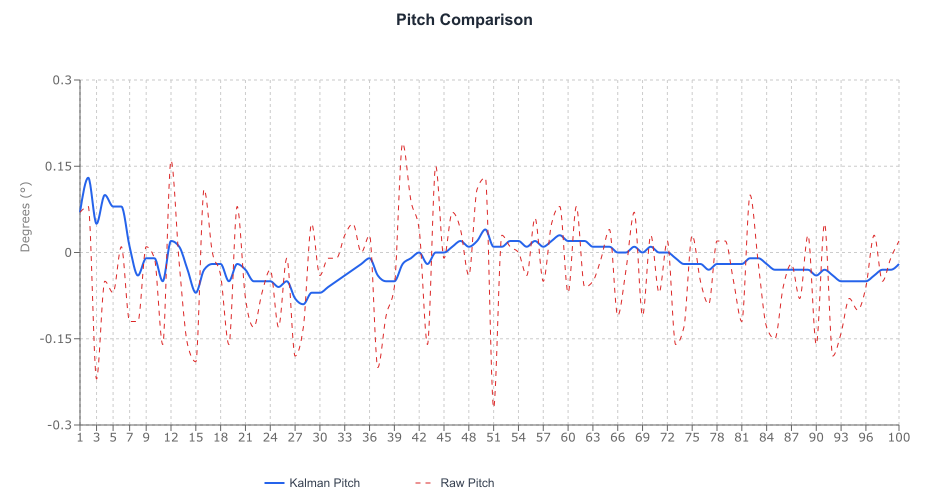
\includegraphics[width=0.8\textwidth]{images/kalman_comparison_pitch_2025-06-23.png}
    \caption{Pitch: Vergleich Rohdaten und Kalman-Filter}
    \label{fig:pitch_pitch}
    \end{figure}

    \begin{figure}[H]
        \centering
        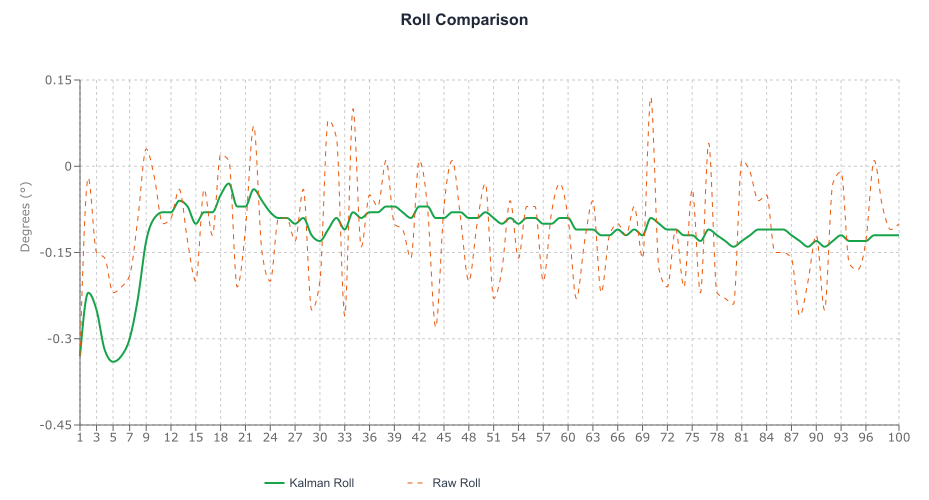
\includegraphics[width=0.8\textwidth]{images/kalman_comparison_roll_2025-06-23.png}
        \caption{Roll: Vergleich Rohdaten und Kalman-Filter}
        \label{fig:roll_roll}
    \end{figure}
\end{samepage}



\section{Gyrosensor Programmierung (Koch)}
Zu Beginn des Projekts war geplant den Gyrosensor MPU6050 zu nutzen, um die Position der Geschützplattform zu bestimmen, da eine kontinuierliche Bewegung um die eigene Achse aufgrund der Kabel nicht möglich ist. Dabei sollte der Sensor über den I2C-Bus mit dem Raspberry Pi 5 verbunden werden, um die Daten auszulesen und zu verarbeiten.
Der MPU6050 ist dabei ein 3-Achsen-Gyroskop und 3-Achsen-Beschleunigungssensor, welcher entsprechende Drehbewegungen und Beschleunigungen entlang der Raumachsen messen kann, welche für eine genaue Winkelbestimmung notwendig sind.

Nach kurzem Einlesen in die Dokumentation waren erste Rohdaten leicht auszulesen. Diese Rohdaten liegen in Form von 16 Bit in zwei Registern bereit und haben die Einheit $\mathit{LSB/g}$ für die Beschleunigungswerte und $\mathit{LSB/^\circ s}$ für die Gyroskop-Werte. Dies gilt es in tatsächliche physikalische Größen umzuwandeln, was bei unserem Projekt letztlich einem Winkel entspricht. 
Um die Beschleunigungswerte nutzen zu können, muss dafür mittels des Skalierungsfaktors die Fallbeschleunigung $\mathit{g}$ errechnet werden, indem man den erhaltenen Wert $x/16384$ rechnet. Die $16384$ ergeben sich aus der Dokumentation und entsprechen den LSB bei einem Messbereich von $\pm2g$, welches der Standardauflösung entspricht und auch die höchste Auflösung des MPU6050 für ist.
Ähnlich wird nun auch Winkelgeschwindigkeit ($\mathit{^\circ s}$) errechnet. Hierbei beträgt der Teiler standardmäßig $131$. \cite[S. 12-13]{raspberry_invensense_mpu6050_datasheet} 

Nach der Umrechnung der Rohdaten in physikalische Größen können nun die Neigungswinkel (Roll- und Pitch-Winkel) des Sensors berechnet werden. Diese ergeben sich aus der Richtung der Erdbeschleunigung relativ zum Sensor. 

Dazu wird die Erweiterung des Arkustangens genutzt, genauer gesagt die Funktion \texttt{atan2}, da sie im Gegensatz zum gewöhnlichen Arctangens auch die Orientierung in allen vier Quadranten berücksichtigt und somit stabile Winkelwerte über den gesamten Bereich von $-180^\circ$ bis $+180^\circ$ liefert. \cite{raspberry_matlab_atan2}

Die Winkelberechnung erfolgt nach der Formel \ref{eq:norms_to_angle}:

\begin{gather}
    \begin{aligned}
    \varphi_\text{pitch} &= \arctan2\left(a_y,\sqrt{a_x^2 + a_z^2}\right) \cdot \frac{180^\circ}{\pi} \\
    \varphi_\text{roll}  &= \arctan2\left(a_x,\sqrt{a_y^2 + a_z^2}\right) \cdot \frac{180^\circ}{\pi}
    \end{aligned}
    \label{eq:norms_to_angle}
\end{gather}


Hierbei sind $a_x$, $a_y$ und $a_z$ die normierten Beschleunigungswerte in $\mathit{g}$ (berechnet aus den Rohwerten durch Division durch $16384$). 

Die $atan2$-Funktion liefert den Winkel zwischen der positiven $x$-Achse und dem Punkt $(x, y)$ in der Ebene, wodurch Sprünge oder Mehrdeutigkeiten bei $90^\circ$ vermieden werden. \cite{raspberry_matlab_atan2}

Nachdem der Term im Code implementiert wurde, konnte ein starkes Rauschen beobachtet werden, was zunächst auf natürliche Schwankungen des Sensors zurückgeführt wurde, weshalb sich dazu entschieden wurde zuerst einen Komplementärfilter zu implementieren,
welcher allerdings das Problem nur bedingt beheben konnte. Deshalb wurde auch noch der Kalman-Filter ausgetestet, wodurch auch eine starke  Rauschunterdrückung festgestellt werden konnte, doch auch hier zeichnete sich ein überdurchschnittliches Rauschverhalten ab, weshalb der Fehler nicht mehr auf ein natürliches Rauschen zurückzuführen war.
Daraufhin wurde auch ein zweiter MPU6050 getestet, welcher ebenfalls dieses Verhalten aufwies, wodurch klar wurde, dass es sich hierbei um einen Programmierfehler handeln muss. Dieser konnte nach einiger Zeit auch herausgefunden werden und lag an der Interpretation der Rohdaten, 
welche fälschlicherweise als \texttt{int16\_t} statt \texttt{uint16\_t} interpretiert wurden.

Aufgrund der aufgewendeten Zeit für die Implementierung des Kalman-Filters sollte dieser aber trotzdem Anwendung im Projekt finden und wird in \ref{sec:kalman_filter} behandelt.

Wie Eingangs erwähnt, sollte der Gyrosensor MPU6050 genutzt werden, um die Position der Geschützplattform zu bestimmen, wofür der Winkel der Drehung um die eigene Achse benötigt wird. Dabei stellte sich heraus das der MPU6050 für diesen Wert zu einem starken Drift neigt, weshalb empfohlen wird diesen mit einem Magnetometer zu kombinieren \cite[S. 26]{raspberry_invensense_mpu6050_datasheet}.
Zur gleichen Zeit stellte sich heraus, dass diese Funktionalität nicht benötigt wird, da über die Servo-Motoren bereits ein Nullpunkt definiert werden konnte, weshalb der Gyrosensor letztlich nur noch für die Neigung der Geschützplattform genutzt wird, um diese als Debug-Information auf dem Webserver \ref{sec:Webserver} anzuzeigen.

\subsection{Kalman Filter Implementierung (Koch)}
\label{sec:kalman_filter}
Der Kalman-Filter ist ein Algorithmus zur Schätzung des Zustands eines dynamischen Systems. Er nutzt Messwerte mit einem mathematischen Modell, um aus verrauschten Daten optimale Schätzungen zu erzeugen und zu filtern, was insbesondere bei Sensoren mit Rauschen, wie dem MPU6050, von Bedeutung ist \cite{raspberry_rwth_kalman_2025}.
Die Berechnung des Kalman-Filters erfolgt nun mittels der Werte des Gyroskops, einer Zeitdifferenz und der zuvor berechneten Roll-und Pitchwinkel. Die Neigungswinkel liefern eine absolute Orientierung relativ zur Erdgravitation, sind jedoch anfällig gegenüber Rauschen und dynamischen Bewegungen, da sie auf Momentanwerten basieren, weshalb man hier auf die Gyroskopwerte zurückgreift.
Diese liefern die Winkelgeschwindigkeit, also die Änderungsrate der Orientierung. Diese Werte werden über die Zeit integriert, um eine relative Winkelschätzung zu erhalten. Sie zeichnen sich durch hohe Kurzzeitstabilität und geringe Reaktionsverzögerung aus, unterliegen jedoch einem Driftverhalten aufgrund von Messabweichungen und systematischen Fehlern.
Der Kalmanfilter fusioniert nun diese beiden Quellen und dessen Vorteile in Relation zum letzten bekannten Zustand.

Dabei besteht der Kalman-Filter aus zwei Hauptphasen: dem Vorhersageschritt (Prediction) und dem Aktualisierungsschritt (Update). Im Vorhersageschritt wird der neue Winkel $\hat{\theta}_{\text{new}}$ basierend auf dem vorherigen Winkel $\hat{\theta}_{\text{prev}}$ und der aktuellen korrigierten Gyroskoprate $\omega$ geschätzt:

\begin{equation*}
\omega = \text{newGyroRate} - \text{bias}, \quad \hat{\theta}_{\text{new}} = \hat{\theta}_{\text{prev}} + dt \cdot \omega
\end{equation*}

Zusätzlich wird die Unsicherheit dieser Vorhersage, dargestellt durch die Kovarianzmatrix $P$, angepasst. Dabei werden sowohl das Zeitintervall $dt$ als auch Modellunsicherheiten, wie der Drift des Gyroskops, berücksichtigt.

Im Aktualisierungsschritt wird der berechnete Winkel $\theta_{\text{meas}}$, welcher mithilfe der Beschleunigungswerte berechnet wurde, mit der Vorhersage verglichen. Die Differenz

\begin{equation*}
S = \theta_{\text{meas}} - \hat{\theta}_{\text{prior}}
\end{equation*}

wird als \emph{Innovation} bezeichnet und wird benötigt um den Kalman-Gain $K$ zu bestimmen. Der Kalman-Gain bestimmt, wie stark diese neue Information zur Korrektur verwendet wird. Er wird aus dem Verhältnis von Unsicherheits-Kovarianzmatrix $P$ und der Innovation $S$ berechnet:

\begin{equation*}
K_0 = \frac{P_{00}}{S}, \quad K_1 = \frac{P_{10}}{S}
\end{equation*}

Hierbei steht $P_{00}$ für die Unsicherheit in der Winkelschätzung, und $P_{10}$ beschreibt die Kovarianz zwischen Winkel und Bias des Gyroskops.

Ein höherer Wert von $K$ bedeutet, dass der Filter der neuen Messung mehr vertraut und ein niedriger Wert zeigt, dass die eigene Vorhersage als zuverlässiger eingeschätzt wird.

Abschließend wird die Kovarianzmatrix $P$ angepasst, um die reduzierte Unsicherheit nach der Messung zu reflektieren. Dadurch wird der Filter präziser in seiner nächsten Schätzung \cite{raspberry_tkjelectronics_kalman_filter_2012}.

Insgesamt erlaubt dieser Algorithmus eine robuste und gleitende Fusion der Sensordaten, wobei kurzfristige Genauigkeit des Gyroskops und langfristige Stabilität des Beschleunigungssensors optimal kombiniert werden.

\begin{samepage}
    In der Abbildung \ref{fig:pitch_pitch} und \ref{fig:roll_roll} ist sowohl für den Pitch, als auch den Roll ein signifikanter Unterschied zwischen den Rohdaten und den gefilterten Daten zu erkennen. Die ersten Schwankungen der gefilterten Werte sind vermutlich genau darauf zurückzuführen, dass der Kalmanfilter mit wenigen Schätzungen noch keinen stabilen Werte für die Kovarianzmatrix und den Bias berechnen konnte, weshalb die Schätzungen auch erst mit steigender Anzahl an Werten genauer werden.
    Der Pitch konnte mithilfe des Kalmanfilters eine Rauschreduktion von $59.4\%$ erzielen und für den Roll $37.4\%$ bei jeweils $100$ Testwerten.

    Aufgrund der Art wie der Gyrosensor auf dem Geschützarm montiert ist, ist für die Neigung allerdings nur der Roll-Wert von Bedeutung.

   \begin{figure}[H]
    \centering
    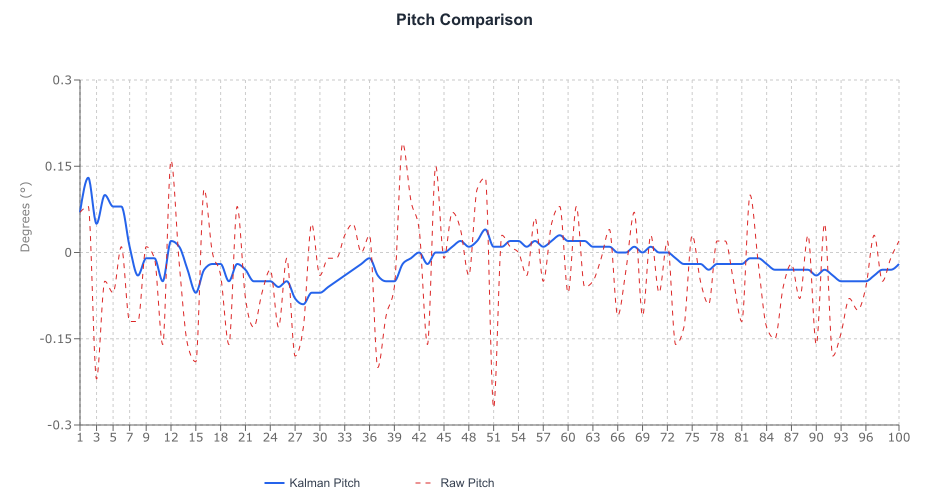
\includegraphics[width=0.8\textwidth]{images/kalman_comparison_pitch_2025-06-23.png}
    \caption{Pitch: Vergleich Rohdaten und Kalman-Filter}
    \label{fig:pitch_pitch}
    \end{figure}

    \begin{figure}[H]
        \centering
        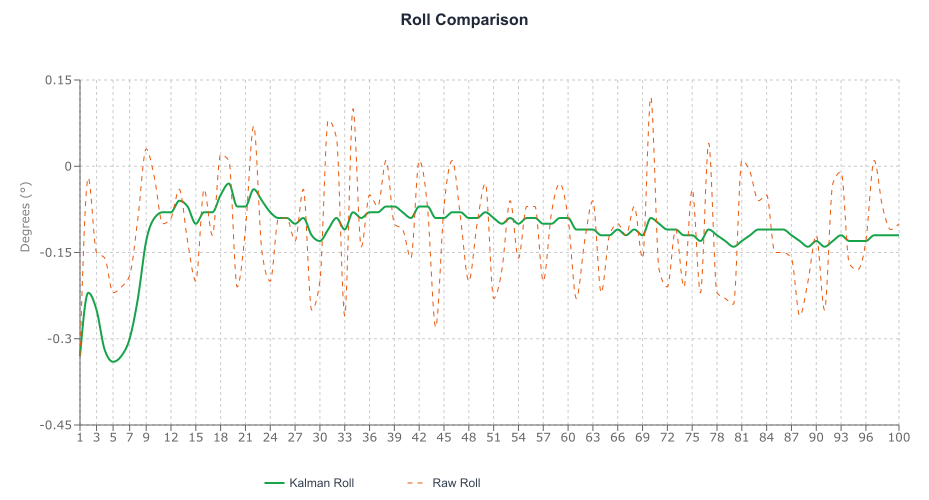
\includegraphics[width=0.8\textwidth]{images/kalman_comparison_roll_2025-06-23.png}
        \caption{Roll: Vergleich Rohdaten und Kalman-Filter}
        \label{fig:roll_roll}
    \end{figure}
\end{samepage}




\chapter{Erstellung \& Ausführung eines KI-Modells zur Objektdetektion} \label{sec:ai_model}
\section{Anforderungen an das KI-Modell (Jürgens)}
Ziel dieser Teilaufgabe war die Entwicklung eines KI-Modells zur automatischen Erkennung eines Holzfliegers als Zielobjekt. Eine zentrale Anforderung bestand darin, das Modell lokal auf einem Raspberry Pi 5 zu implementieren und auch dort auszuführen. Aufgrund der fehlenden dedizierten Grafikkarte des Systems war ein leichtgewichtiges, CPU-optimiertes Modell erforderlich. Der verwendete Raspberry Pi 5 verfügt über einen 64-Bit Quad-Core ARM Cortex-A76 Prozessor und 8 GB Arbeitsspeicher. \cite{raspberrypi5website} 
Aufgrund dieser Hardwarebeschränkung und persönlicher Erfahrungen wurde entschieden, dass ein YOLO Modell des Unternehmens Ultralytics verwendet wird. Dieses hat sich auf state-of-the-art KI-Modellen der YOLO-Familie im Bereich der Objekterkennung und Bildsegmentierung spezialisiert. \cite{ultralyticsFAQ} Die Modelle von Ultralytics zeichnen sich durch eine hohe Präzision und schnelle Inferenzzeiten aus. Diese Eigenschaften sind für die lokale Ausführung auf dem Raspberry Pi 5 von großer Bedeutung, da hier die Inferenz auf der CPU durchgeführt werden muss. 
Besonders interessant sind die Open-Source Implementierungen der YOLOv8 und YOLOv11 Modelle. Diese sind bereits vortrainiert und haben bestehende Gewichte und bieten somit die Möglichkeit direkt verwendet oder auf einem eigenen Datensatz weitertrainiert zu werden. Ein weiterer Vorteil der YOLO Modelle und Ultralytics liegt in der sehr guten Dokumentation und einer geringen Einstiegshürde. Mit der Ultralytics Python Bibliothek können Modelle einfach erstellt, trainiert und evaluiert werden. Dies bildet die Grundlage für die Entwicklung und Verwendung des Modells in diesem Projekt.


\section{Modellauswahl (Jürgens)}
Die YOLOv8 und YOLOv11 Modelle von Ultralytics werden in verschiedenen Größen angeboten. Mit steigender Größe des Modells steigt zwar die Genauigkeit des Modells, aber auch die Inferenzzeit und der Speicherbedarf.
Die Modelle werden in folgenden Größen angeboten:
\begin{itemize}
    \item YOLOv8/11n - Nano 
    \item YOLOv8/11s - Small
    \item YOLOv8/11m - Medium
    \item YOLOv8/11l - Large
    \item YOLOv8/11x - Extra Large
\end{itemize}
Die Modellauswahl ist durch die Hardware des Raspberry Pi 5 begrenzt. So sind insbesondere die mittleren und großen Modelle aufgrund der hohen Inferenzzeiten nicht für die Ausführung auf der CPU des Raspberry Pi 5 geeignet. Bereits das YOLOv8m Modell hat eine Inferenzzeit von 234,7 ms. \cite{ultralyticsYOLOv8Performance} Anhand dessen wurde entschieden, dass eine Beschränkung auf die kleineren Modelle YOLOv8n, YOLOv8s, YOLO11n und YOLO11s sinnvoll ist. Diese Modelle haben eine geringere Inferenzzeit und könnten somit besser für die Ausführung auf dem Raspberry Pi 5 geeignet sein. 
Die folgenden Leistungsmetriken stammen aus der offiziellen Online-Dokumentation von Ultralytics [\cite{yolov8_ultralytics,ultralyticsYOLOv8Performance,yolo11_ultralytics}]:
\begin{itemize}
    \item YOLOv8n $\approx$ 80.4 ms
    \item YOLOv8s $\approx$ 128.4 ms
    \item YOLO11n $\approx$ 56.1 ms 
    \item YOLO11s $\approx$ 90.0 ms 
\end{itemize}

Anhand dieser Werte und persönlicher Erfahrungen wurde zunächst entschieden, dass das YOLOv8n Modell im ONNX-Format verwendet wird. Dieses Modell hat mit einer Inferenzzeit von 80,4 ms eine vertretbare Geschwindigkeit.

\subsection{Das ONNX-Format (Jürgens)}
ONNX steht für Open Neural Network Exchange und stellt ein Open-Source-Format für KI-Modelle bereit. Es ermöglicht KI-Modelle über verschiedene Frameworks und Plattformen hinweg zu verwenden. Modelle können beispielweise in einem Framework mit PyTorch trainiert und anschließend in das ONNX-Format exportiert werden. Oftmals ermöglicht die Verwendung des ONNX-Formats eine bessere Performance von KI-Modellen auf verschiedenen Hardwareplattformen durch optimierte Inferenzmaschinen. \cite{ultralyticsGlossaryONNX}

Der Ansatz für dieses Projekt war es, ein Modell auf einer leistungsstarken Maschine mit dedizierter Grafikkarte zu trainieren und dieses anschließend in das ONNX-Format zu exportieren. Die Python Bibliothek von Ultralytics bietet unter Anderem die Möglichkeit ein Modell zu trainieren und anschließend in das ONNX-Format zu exportieren. Nach dem Training hat das Modell zunächst das PyTorch-Format mit der Dateiendung \texttt{.pt}.
Nach dem Export in das ONNX-Format hat das Modell die Dateiendung \texttt{.onnx}. Dieses Format kann beispielsweise mit Tools wie NVIDIA TensorRT oder Intels OpenVINO optimiert werden. Laufzeitumgebungen wie ONNX Runtime sind dabei für Hochleistungsinferenz über verschiedene Hardware optimiert. \cite{ultralyticsGlossaryONNX}


\section{Trainingsdaten \& Annotation (Jürgens)}
Die Qualität und Performance eines KI-Modells hängt maßgeblich von der Qualität der Trainingsdaten ab. Der erste Schritt ist es, einen qualitativ hochwertigen Datensatz zum Trainieren des Modells zu erstellen. Das Ziel ist es endgültig einen Holzflieger auf einem Bild zu erkennen. Die Trainingsdaten wurden direkt mit dem Raspberry Camera Module 3 aufgenommen, welches mit einer Auflösung von 11,9 Megapixeln und einer Bittiefe von 24 Bit bei einer Bildgröße von 4608x2592 Pixeln arbeitet. \cite{raspberrypi5cammodule3} Die Kamera wird neben der Erstellung der Trainingsdaten auch für die Inferenz des Modells im späteren Verlauf verwendet. 
Um eine robuste Objekterkennung unabhängig von der räumlichen Orientierung des Zielobjekts zu gewährleisten, wurde ein Datensatz von 1.201 Bildern erstellt. Diese umfassen verschiedene Umgebungsbedingungen, Beleuchtungssituationen und Perspektiven, wobei das Zielobjekt in nahezu allen möglichen Neigungen erfasst wurde.
Für das überwachte Lernverfahren sind neben den Bilddaten entsprechende Annotationen erforderlich. Der Annotationsprozess erfordert die manuelle Markierung der zu erkennenden Objekte in einem geeigneten Tool sowie deren Konvertierung in ein kompatibles Format. Dieser arbeitsintensive Prozess ist von entscheidender Bedeutung, da die Qualität der Annotationen direkt die Modellperformanz beeinflusst. Vor Beginn des Annotationsprozesses muss zunächst die Art der Annotierung definiert werden.
Für diese Arbeit gab es zwei Arten der Annotation, die in Betracht gezogen wurden:
\begin{itemize}
    \item Bounding Box: Ein Rechteck wird um das zu erkennende Objekt gezeichnet. Diese Methode ist einfach und schnell, aber weniger präzise.
    \item Polygon: Eine komplexere Form wird um das Objekt gezeichnet. Diese Methode ist genauer, aber auch zeitaufwändiger.
\end{itemize}
Die Entscheidung fiel auf die zeitaufwändigere Polygon-Annotation. Diese ermöglicht eine genauere Erkennung des Holzfliegers weil nicht nur die äußeren Kanten sondern auch die komplexere Form des Objekts berücksichtigt wird. 
Neben der speziellen Form des Holzfliegers war diese Entscheidung auch durch die relativ geringe Anzahl vorhandener Trainingsbilder begründet. 
Zur Annotation wurde das Open-Source Tool LabelStudio verwendet. Dieses bietet eine benutzerfreundliche Oberfläche und lässt sich sehr genau personalisieren. Durch die integrierte Projektverwaltung und verschiedener unterstützter Exportformate bietet das Tool eine gute Lösung für die Annotierung.
Aufgrund fehlender Implementation der Exportfunktion für größere Datensätze (Export von Bildern und korrespondierenden Annotationen) war eine Nachbereitung des Datensatzes notwendig. Nach Abschluss der Annotation wurden die Labels im YOLO-Format exportiert und eine Ordnerstruktur erstellt, die zum Training des YOLO-Modells verwendet werden kann.
\\ Folgende Ordnerstruktur wurde erstellt: \\ 

\dirtree{%
.1 train/.
.2 images/.
.2 labels/.
.1 val/.
.2 images/.
.2 labels/.
.1 test/.
.2 images/.
.2 labels/.
}

\newpage
Die Bilder und Labels im Ordner \texttt{train} werden für das Training des Modells verwendet, die Bilder und Labels im Ordner \texttt{val} für die Validierung des Modells während des Trainings und die Bilder und Labels im Ordner \texttt{test} für die abschließende Evaluation des Modells.
Die Bilder wurden in den Ordnern \texttt{images} und die Annotationen in den Ordnern \texttt{labels} gespeichert. Die Annotationen werden in Textdateien mit der Endung \texttt{.txt} gespeichert, wobei jede Textdatei die gleiche Bezeichnung wie das zugehörige Bild hat. Beispielsweise wird das Bild \texttt{image1.jpg} im Ordner \texttt{images} durch die Textdatei \texttt{image1.txt} im Ordner \texttt{labels} annotiert.


\section{Training des Modells (Jürgens)}
Ultralytics bietet mit der Python-Bibliothek \texttt{ultralytics} eine einfache Möglichkeit, ein YOLO-Modell zu trainieren, zu validieren und zu evaluieren. Vor dem Training wird eine Konfigurationsdatei benötigt, welche die Pfade des Trainingsordners, des Validierungsordners und des Testordner enthält. Neben den Pfaden beinhaltet Sie noch die Anzahl der Klassen und den dazugehörigen Namen. In diesem Fall gibt es nur den Holzflieger als Klasse, welcher zukünftig mit der Bezeichnung 'Plane' gelabelt wird. \newline

Das Training erfolgt auf einer Mittelklasse NVIDIA Grafikkarte (RTX 3070) mit 8 GB Grafikkartenspeicher und wurden der offiziellen NVIDIA Produktseite entnommen.\cite{RTX3070Specs} Während des Trainings werden die Trainingsbilder augmentiert, um die Robustheit des Modells zu erhöhen. So werden verschiedene Transformationen auf die Bilder angewendet, wie z.B. Rotation, Skalierung oder Änderung der Helligkeit. Hiermit wird die Varianz der Trainingsbilder künstlich erhöht, was zu einer besseren Performance des Modells führt. \cite{YoloDataAugmentation} Durch das Verwenden von vortrainierten Gewichten wird die Trainingszeit verkürzt und die Performance des Modells verbessert. Diese vortrainierten Gewichte werden vor dem Trainings als \texttt{.pt} Datei heruntergeladen und bereitgestellt und bieten den Ausgangspunkt für das Training. Durch Transferlearning, also dem weitertrainieren eines vortrainierten Modells auf einen neuen Datensatz, kann die Performance des Modells weiter verbessert werden. Zudem wird die benötigte Trainingszeit reduziert. \cite{TransferLearningGlossary}


Nach Abschluss des Trainings werden automatisch die besten Gewichte des Modells unter \texttt{runs/detect/train/weights/best.pt} gespeichert. Neben den reinen Gewichten erstellt das Trainingsskript unter Anderem die Datei \texttt{results.png} in welcher verschiedene Metriken des Trainings, wie zum Beispiel die \texttt{mAP50} und \texttt{mAP50-95}, visualisiert werden. Die Metrik \texttt{mean Average Precision} wie zum Beispiel \texttt{mAP50} und \texttt{mAP50-95} geben die Genauigkeit des Modells an, wobei \texttt{mAP50} die Genauigkeit bei einer IoU-Grenze von 0,5 und \texttt{mAP50-95} bei IoU-Werten zwischen 0,5 und 0,95 angibt \cite{MAPGlossary}. IoU steht für Intersection over Union und gibt die prozentuale Schnittmenge zwischen der vorhergesagten Bounding Box und der tatsächlichen Bounding Box an.\cite{IOUGlossary}
So kann man sagen, dass ein hoher \texttt{mAP50}-Wert und \texttt{mAP50-95}-Wert gute Indikatoren sind wie gut das Modell die Objekte erkennt. \newpage



\begin{figure}[h]
  \centering
  \begin{subfigure}[b]{0.45\textwidth}
    \centering
    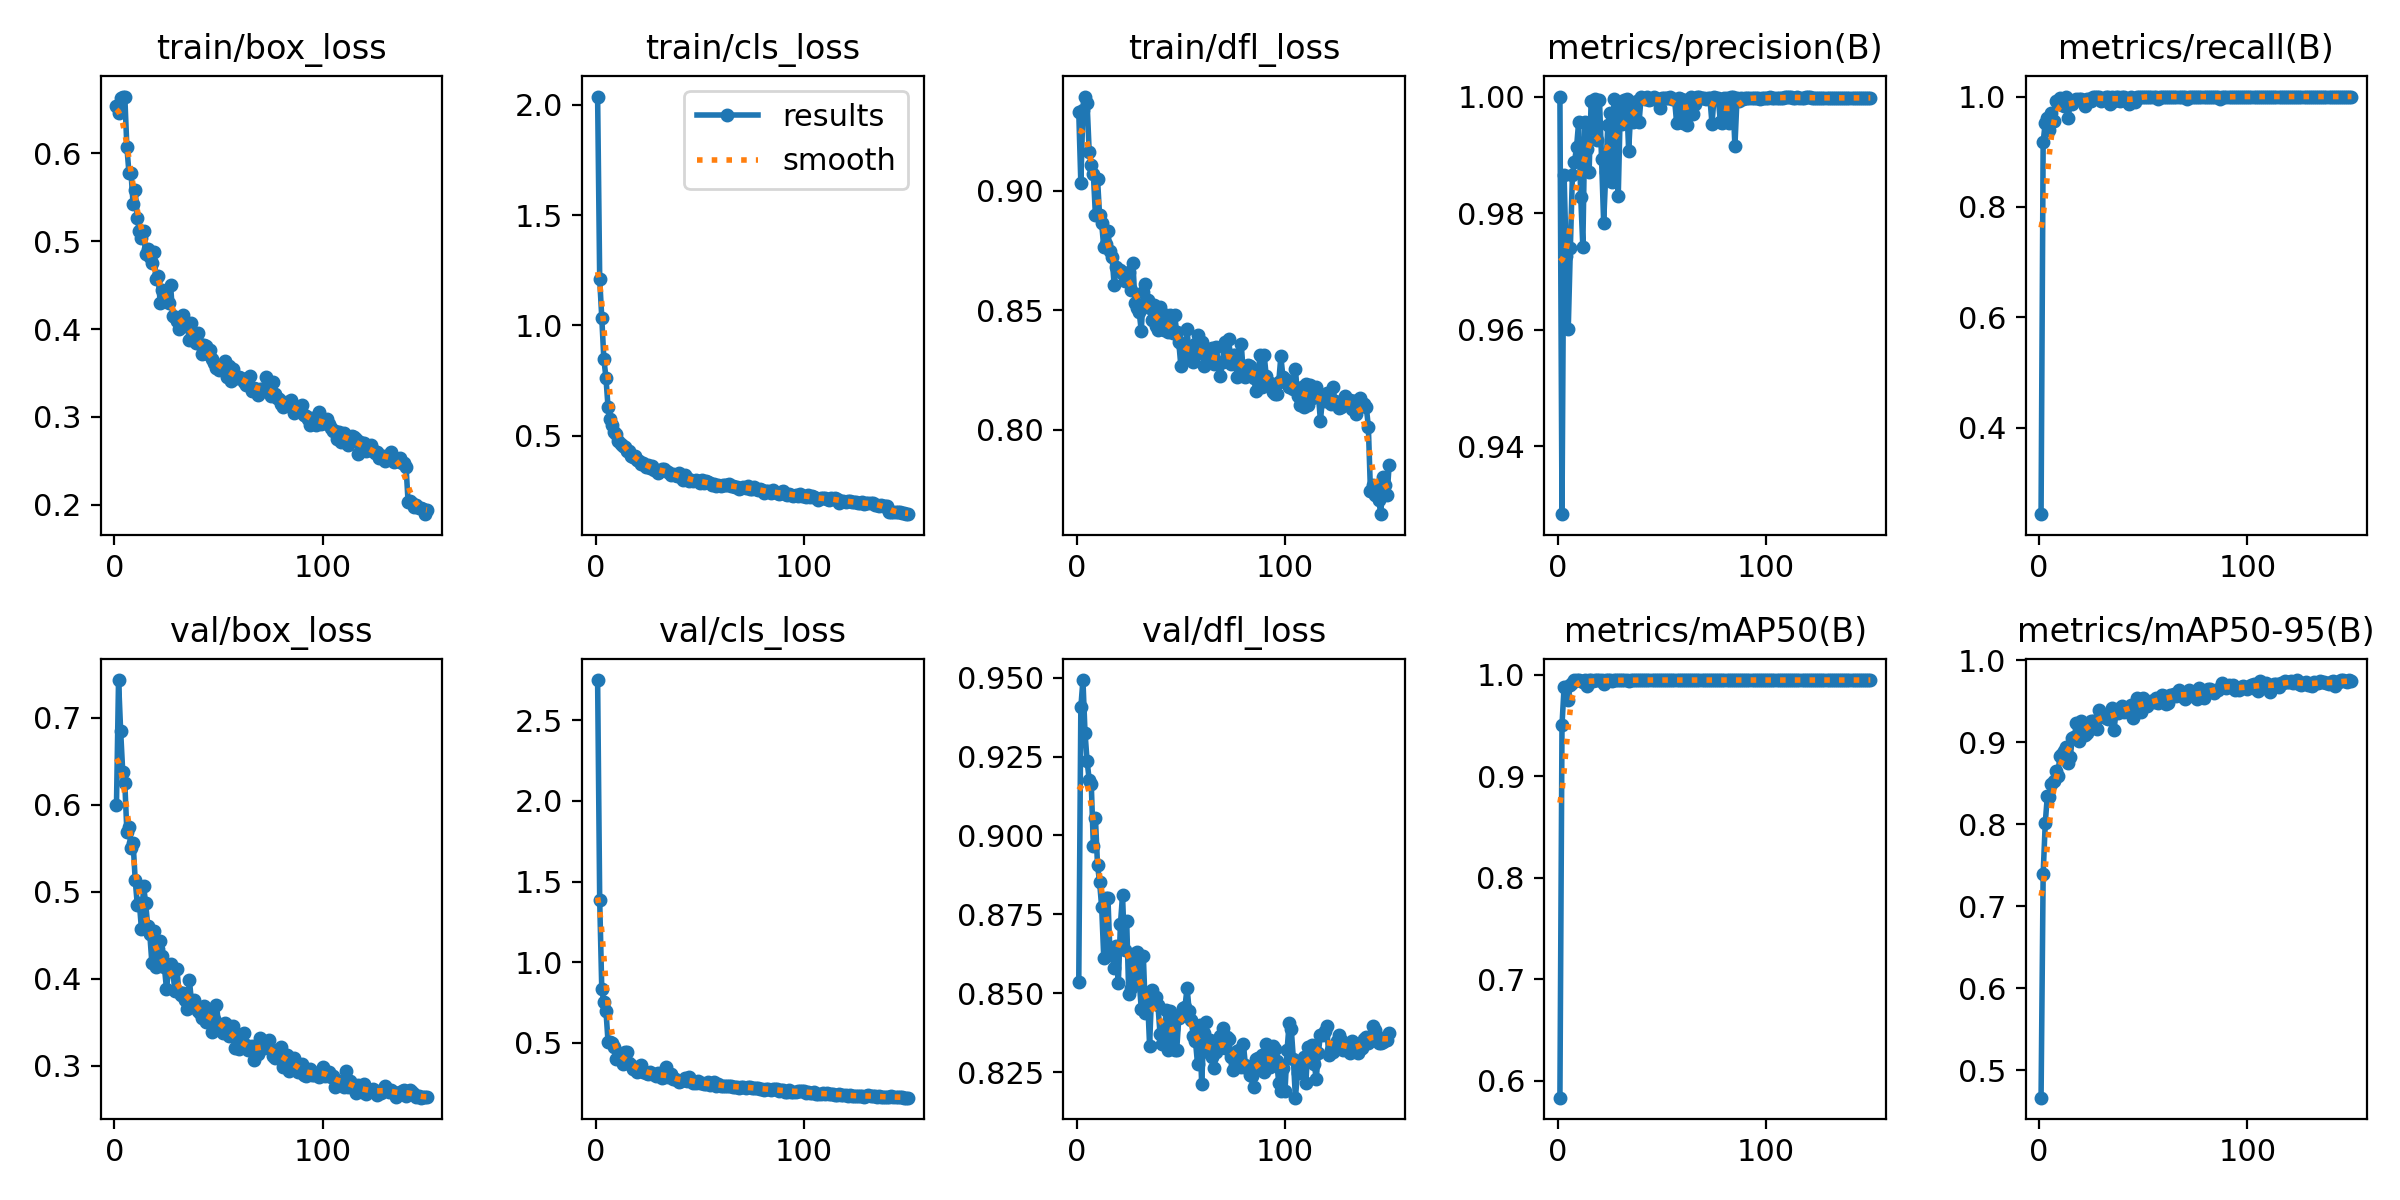
\includegraphics[width=0.9\textwidth]{images/Trainingsresults_yolov8n.png}
    \caption{YOLOv8n}
    \label{fig:Trainingsresultate yolov8n}
  \end{subfigure}
  \hfill
  \begin{subfigure}[b]{0.45\textwidth}
    \centering
    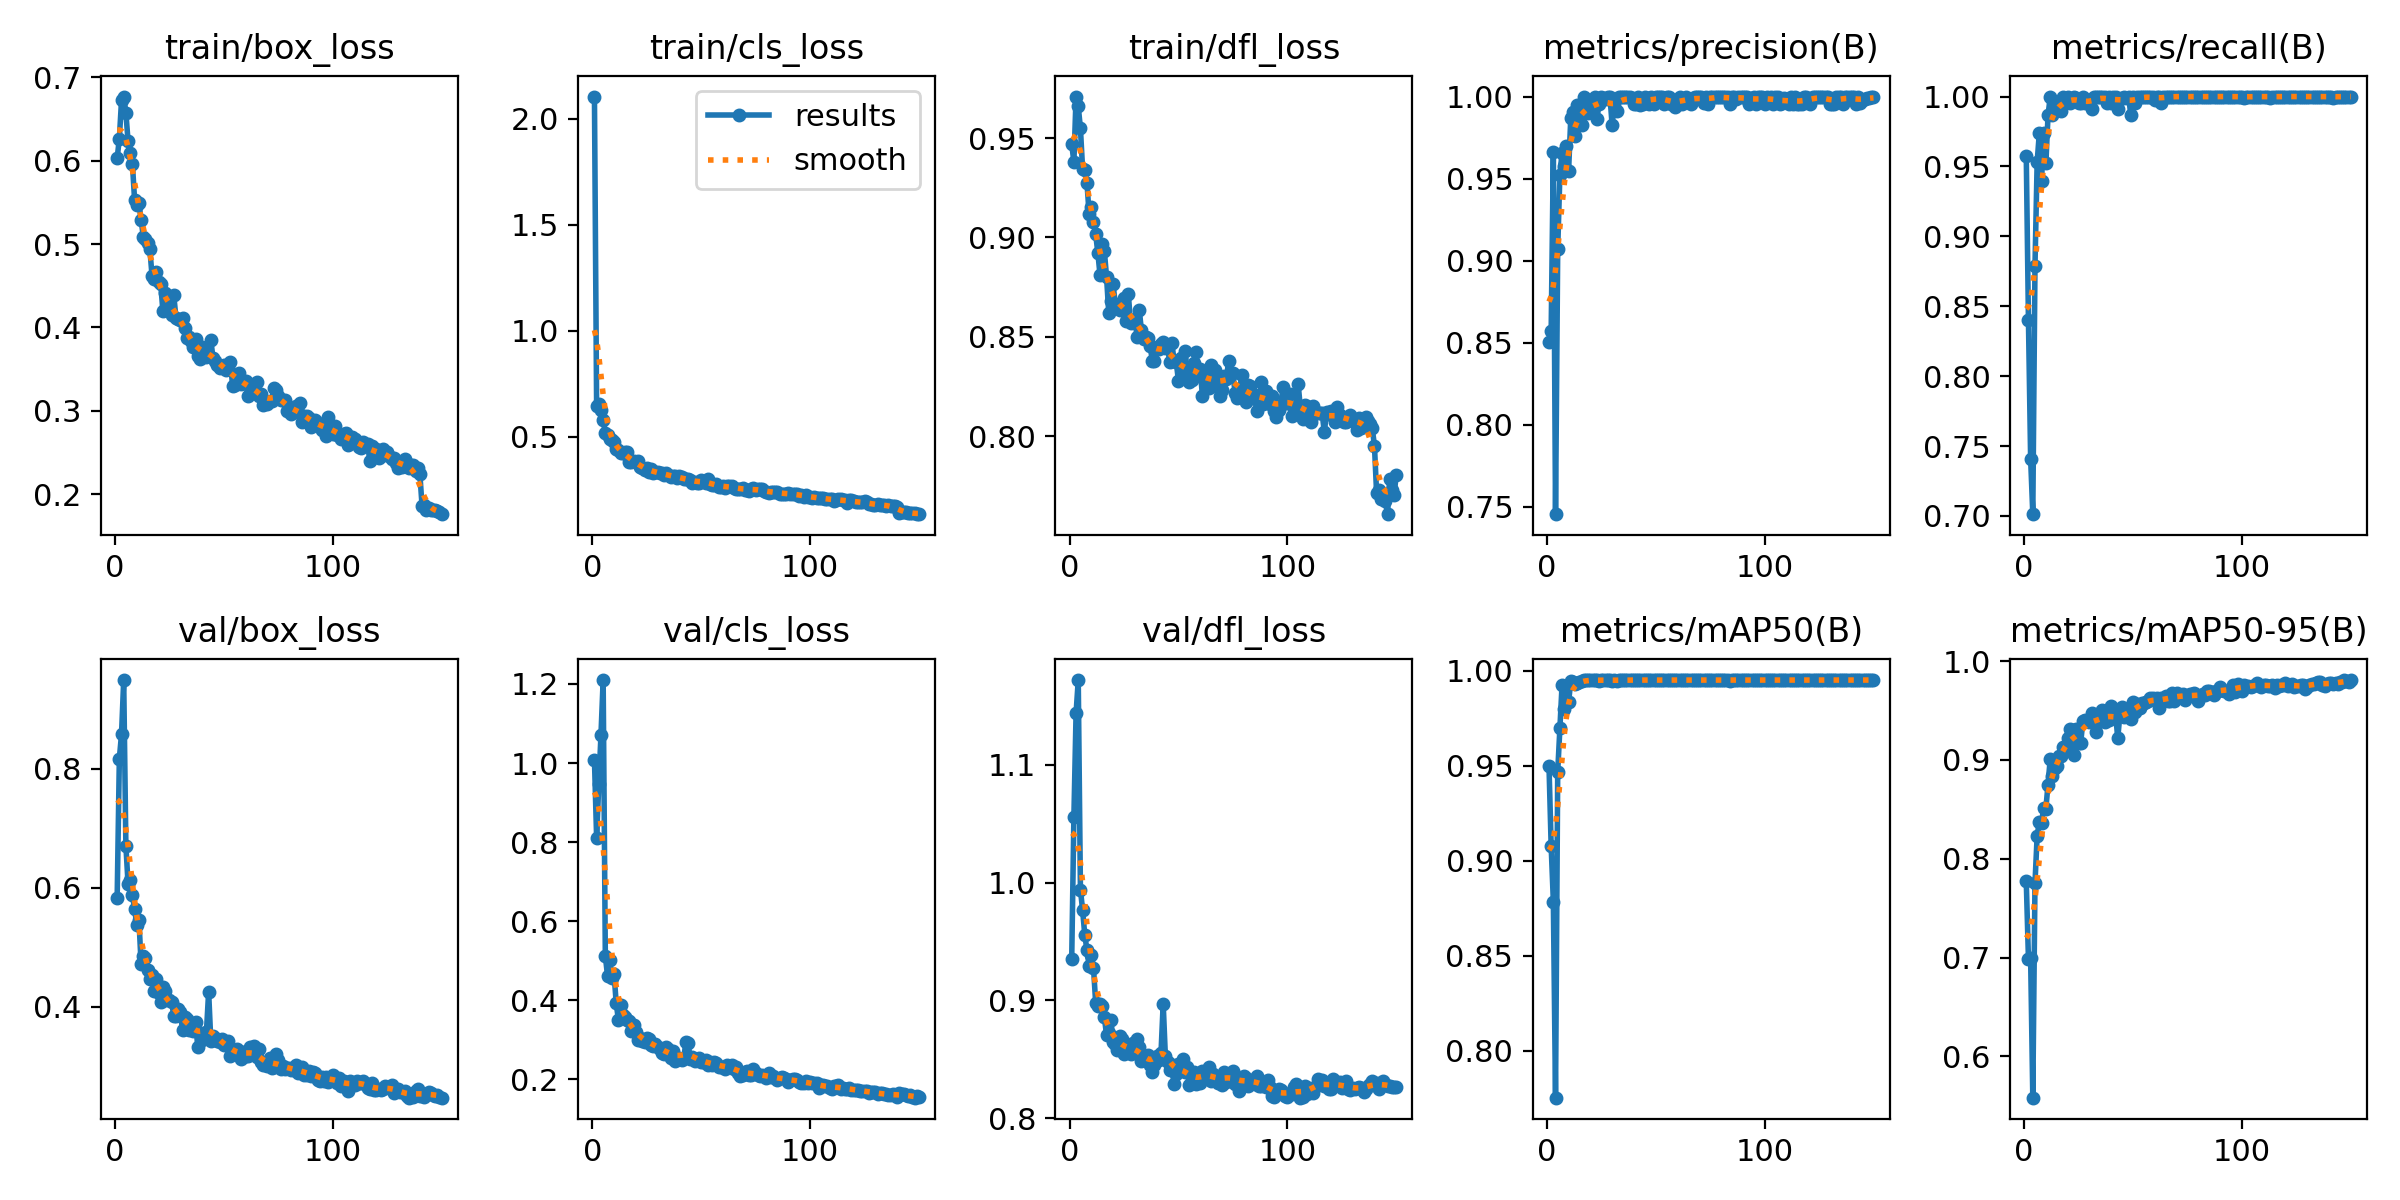
\includegraphics[width=0.9\textwidth]{images/Trainingsresults_yolov8s.png}
    \caption{YOLOv8s}
    \label{fig:Trainingsresultate yolov8s}
  \end{subfigure}
  \vskip\baselineskip
  \begin{subfigure}[b]{0.45\textwidth}
    \centering
    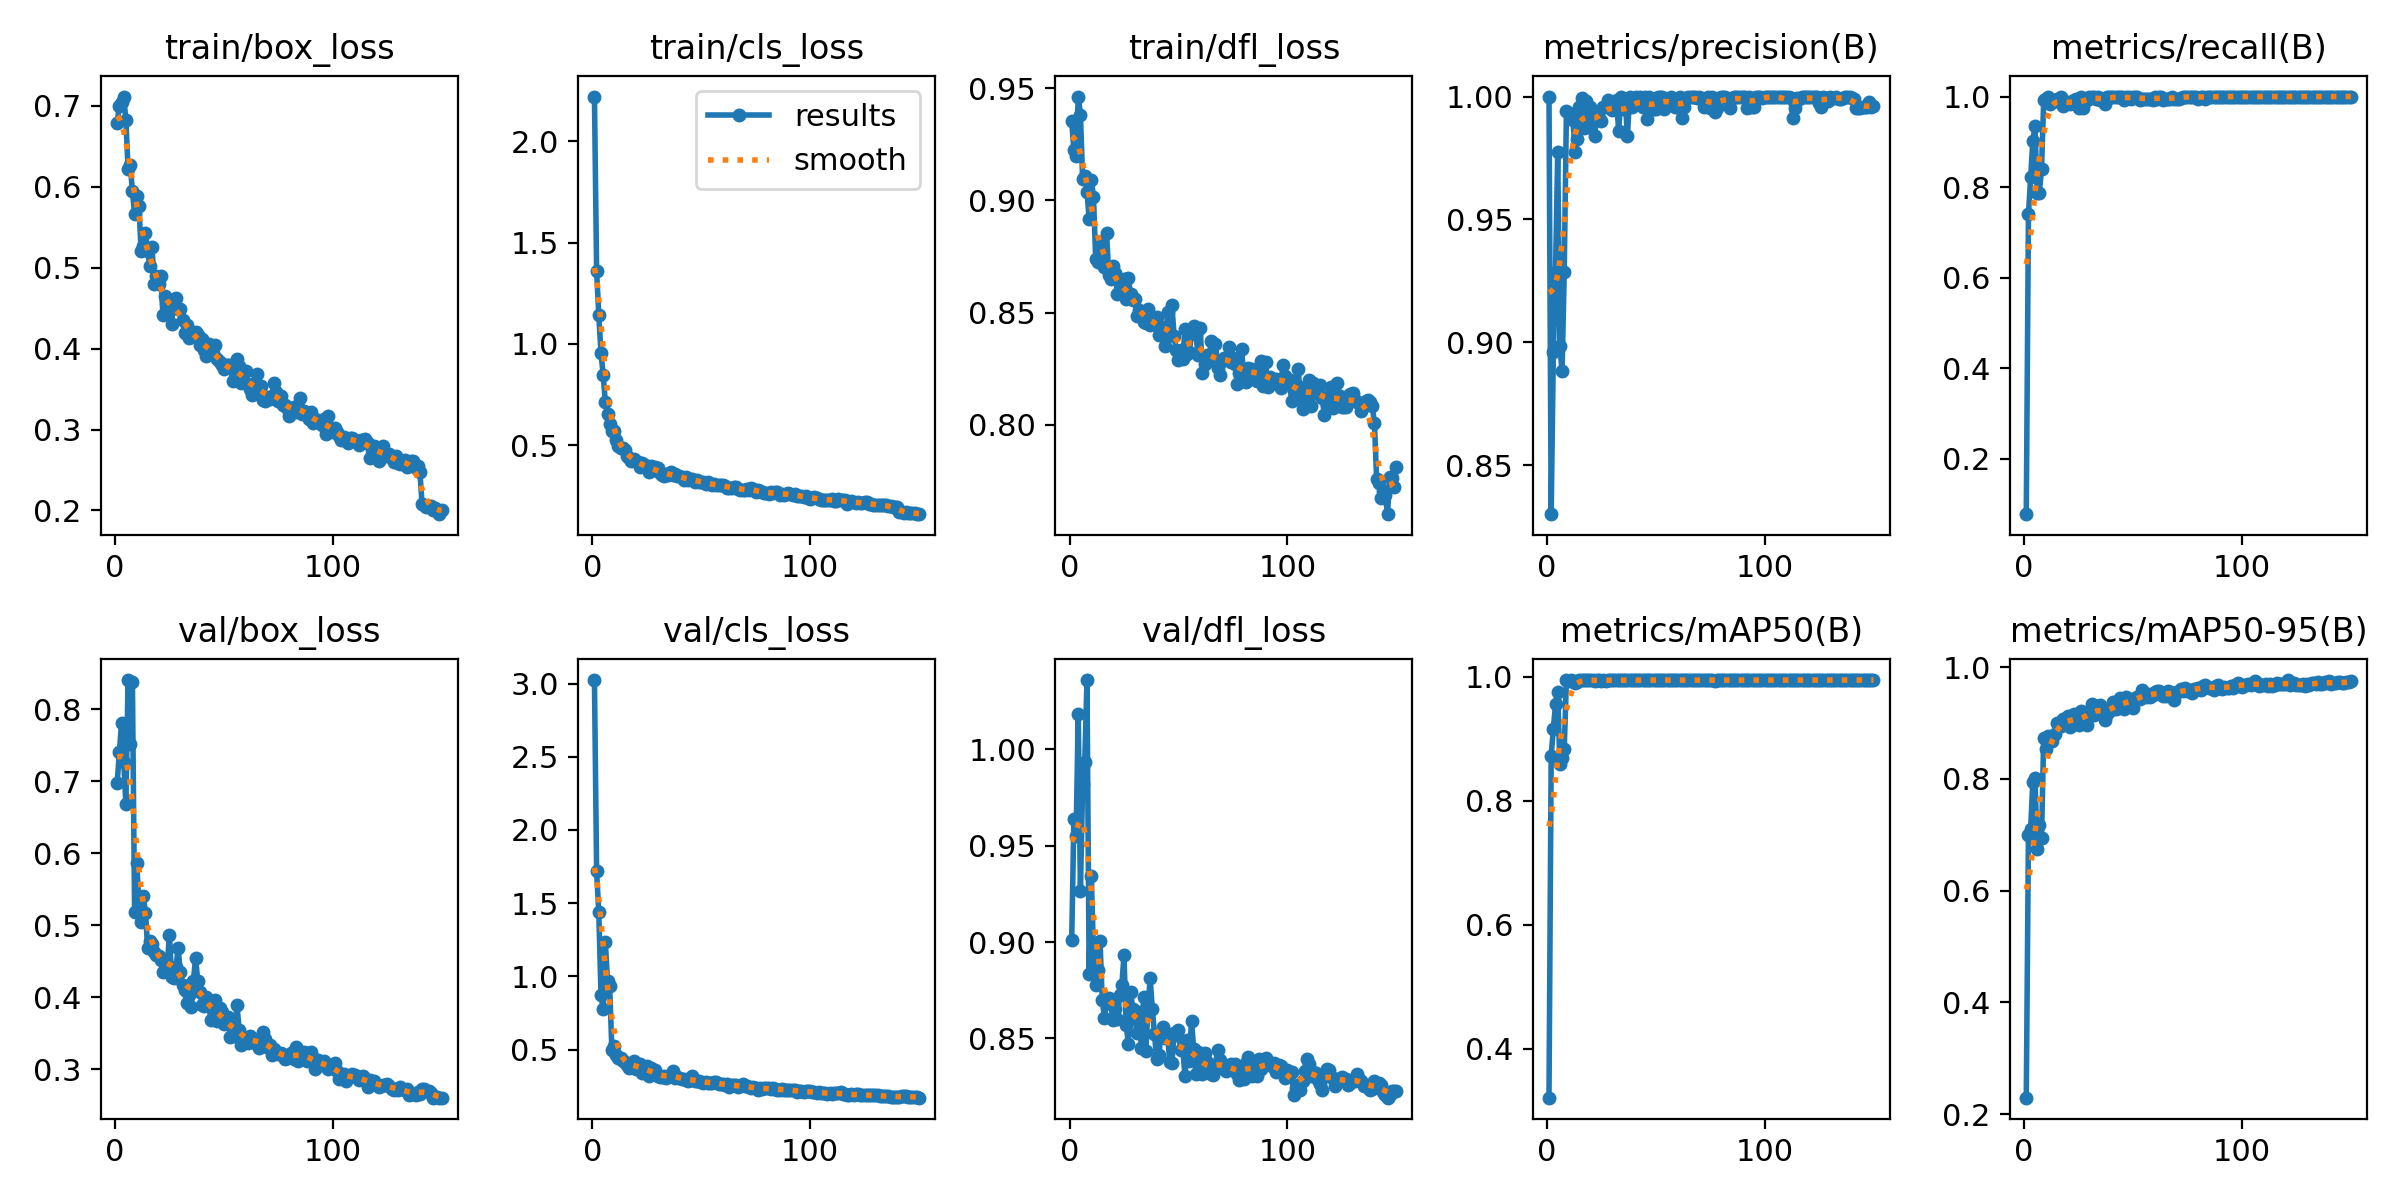
\includegraphics[width=0.9\textwidth]{images/Trainingsresults_yolo11n.png}
    \caption{YOLO11n}
    \label{fig:Trainingsresultate yolo11n}
  \end{subfigure}
  \hfill
  \begin{subfigure}[b]{0.45\textwidth}
    \centering
    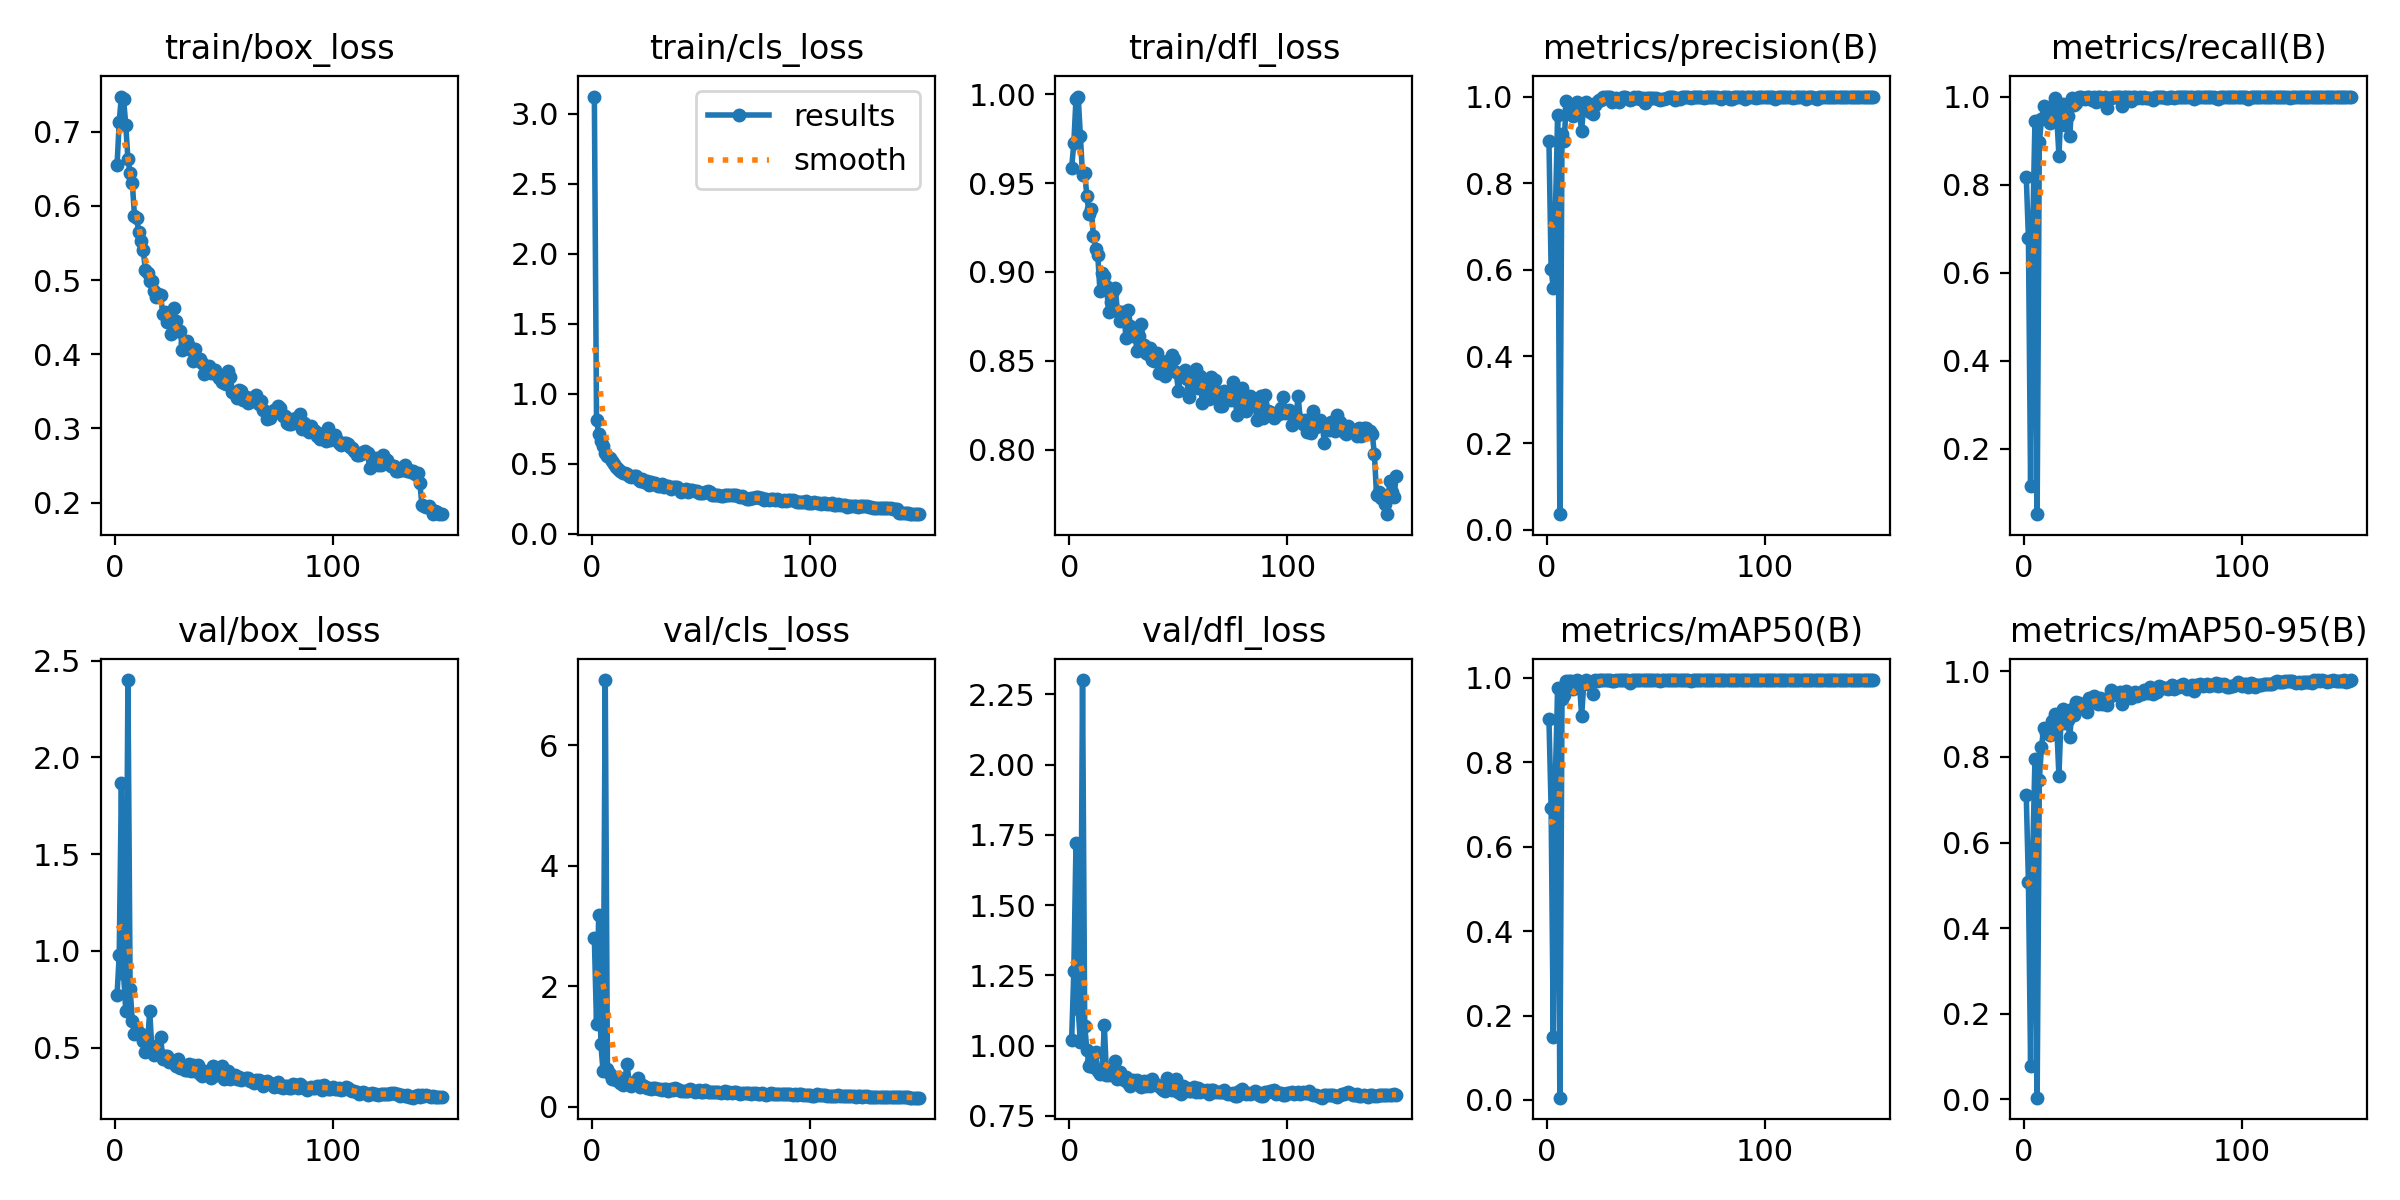
\includegraphics[width=0.9\textwidth]{images/Trainingsresults_yolo11s.png}
    \caption{YOLO11s}
    \label{fig:Trainingsresultate yolo11s}
  \end{subfigure}
  \caption{Vergleich Trainingsresultate YOLOv8n, YOLOv8s, YOLO11n und YOLO11s}
  \label{tab:Vergleich Trainingsresultate}
\end{figure}



Wie in \ref{tab:Vergleich Trainingsresultate} zu sehen ist, schneiden alle Modelle nach der Trainingsphase von 150 Epochen ähnlich gut ab. Eine Epoche stellt dabei ein vollständiger Durchlauf durch den gesamten Trainingsdatensatz dar.\cite{EpochGlossary} Anhand dieser Resultate wurde zunächst das YOLOv8n Modell ausgewählt, da es entsprechend der Trainingsmetriken trotz der geringeren Größe im Vergleich zu den s-Modellen eine ähnlich gute Performance aufweist dabei aber eine geringe Inferenzzeit aufweist. Dazu kommen positive persönliche Erfahrungen mit dem YOLOv8n Modell. 


Um das Modell schließlich auch als ONNX-Modell zu betreiben muss dieses zunächst in das ONNX-Format exportiert werden. Der Export erfolgt mit der Ultralytics Python-Bibliothek.

\section{Ausführung des Modells im ONNX-Format (Jürgens)}
Um generell ein KI-Modell im ONNX-Format auszuführen, sind einige Voraussetzung an das System zu erfüllen. Es werden verschieden Programme und Bibliotheken benötigt, um das Modell auszuführen. Um schnelle Ergebnisse und erstes Feedback zu erhalten wie die Inferenz des Modells im ONNX-Format abläuft wurde zunächst eine Laufzeitumgebung auf dem persönlichen Computer eingerichtet. Folgende Bibliotheken und Programme waren auf jeden Fall notwendig, um das Modell auszuführen:

\begin{itemize}
    \item ONNX Runtime v1.21.0
    \item OpenCV (mit GStreamer Unterstützung)
    \item CUDA 12.6 (optional, für GPU-Beschleunigung)
    \item cuDNN 9.9 (NVIDIA Deep Neural Network library, NVIDIA Developer Account erforderlich)
\end{itemize}

\newpage
Zwischen diesen Komponenten gibt es Abhängigkeiten speziell in der Versionierung. So muss beispielsweise die CUDA-Version zur eingesetzten Grafikkarte und die cuDNN-Version zur CUDA-Version passen. \\ Um den Anforderungen einer minimalen Laufzeit pro Inferenz gerecht zu werden, war die Zielprogrammiersprache C++ und nicht Python. Aufgrund fehlender Erfahrungen mit KI-Modellen im ONNX-Format wurde die Erstellung eines ersten Prototypen mit Hilfe von ChatGPT und der ONNX-Dokumentation gelöst. Es stellte sich heraus, dass die Ergebnisse der Inferenz im ONNX-Format mangelhaft sind, wobei man eine fehlerhafte Implementierung im C/C++ Code nicht ausschließen kann. Im Vergleich zu den Ergebnissen der Inferenz mit der von Ultralytics bereitgestellten Python-Bibliothek kann man die Ergebnisse der Inferenz des C/C++ Prototypen nicht verwenden. Um ein vergleichbares Ergbnis zu produzieren, werden beide Inferenzen mit dem selben Video getestet. Das Video wurde direkt mit dem Raspberry Pi 5 und dem Camera Module 3 aufgenommen.

\begin{figure}[h]
  \centering
  \begin{subfigure}[b]{0.48\textwidth}
    \centering
    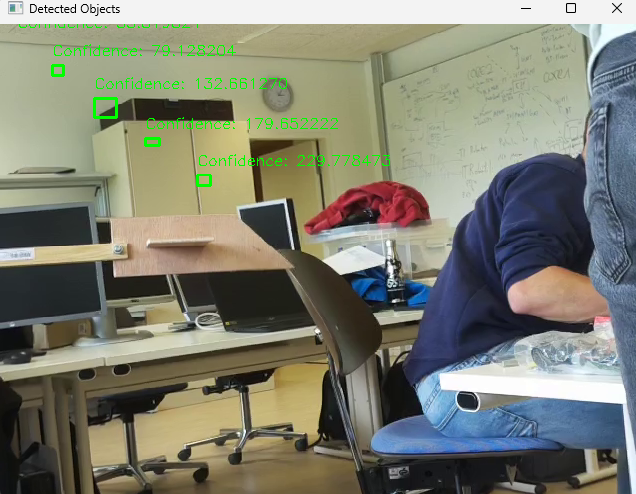
\includegraphics[width=0.9\textwidth,height=5.9cm,keepaspectratio]{images/ONNX_Inferenz.png}
    \caption{Inferenz im ONNX-Format mit C++ Prototypen}
    \label{fig:Screenshot: Inferenz im ONNX-Format mit C++ Prototypen}
  \end{subfigure}
  \hfill
  \begin{subfigure}[b]{0.48\textwidth}
    \centering
    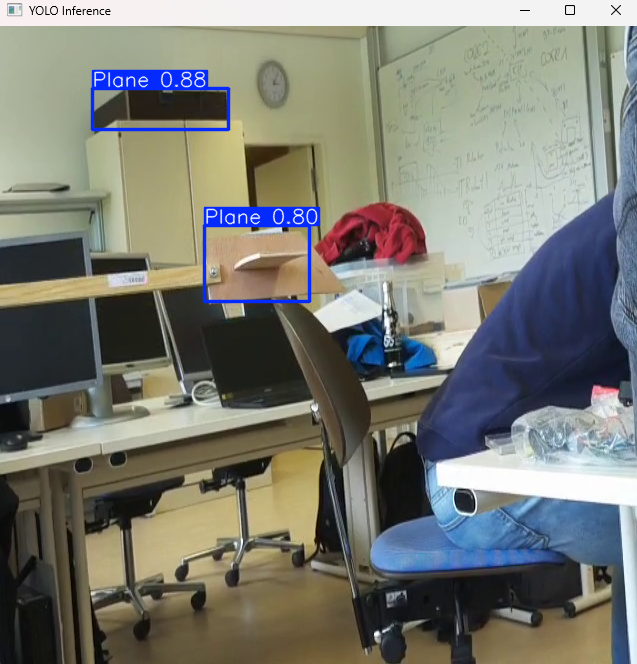
\includegraphics[width=0.9\textwidth,height=6.2cm,keepaspectratio]{images/Python_Inferenz.png}
    \caption{Inferenz in Python mit Ultralytics}
    \label{fig:Screenshot: Inferenz Python mit Ultralytics}
  \end{subfigure}
  \caption{Vergleich Inferenz ONNX C++ und Python}
  \label{tab:Vergleich Inferenz ONNX C++ und Python}
\end{figure}

Wie in \ref{tab:Vergleich Inferenz ONNX C++ und Python} zu sehen ist, sind die Ergebnisse der Inferenz in Python mit der Ultralytics-Bibliothek deutlich besser.
Basierend auf diesen Resultaten wurde entschieden, dass eine weitere Implementierung in C/C++ nicht sinnvoll ist. So fällt besonders die hohe Komplexität, die fehlerhaften Erkennungen, die hohe Einarbeitungszeit hinsichtlich der Projektdauer, aber auch der hohe Aufwand für die Einrichtung einer funktionierenden Laufzeitumgebung ins Gewicht. Mit der Verwendung der Ultralytics Bibliothek fällt ein Großteil dieser Komplexität weg. 

\section{Inferenz des PyTorch-Modells (Jürgens)}

\subsection{Installation der KI-Abhängigkeiten (Jürgens)} 
Neben der reinen Ultralytics-Bibliothek welche mit einer Reihe weiterer Abhängigkeiten installiert wird, ist besonders die Python-Version von \texttt{OpenCV} von Bedeutung. 
OpenCV ist größtenteils in C++ geschrieben, bietet aber auch eine Python-Schnittstelle an. Diese soll dafür verwendet werden, um auf den Kamera-Stream des Raspberry Pi 5 zuzugreifen und bildet die Grundlage für die Inferenz mit dem YOLO-Modell. 
In der Regel kann ein Stream in OpenCV mit der Funktion \texttt{cv2.VideoCapture()} geöffnet werden. Der Stream kann dabei eine angebundene Kamera, eine Videodatei oder auch ein RTSP-Stream sein. Aufgrund fehlender Unterstützung des Kamera-Softwarestacks des Raspberry Pi 5 kann die Kamera nicht direkt mit der Funktion \texttt{cv2.VideoCapture()} geöffnet werden \ref{opencvlibcamera}. Der Test mit einer USB-Kamera dagegen funktionierte problemlos. Da OpenCV eine essenzielle Abhängigkeit in diesem Projekt ist, wurde ein Workaround gefunden in dem die Kamera des Raspberry Pi 5 mittels GStreamer an OpenCV übergeben wird. Eine reguläre OpenCV-Installation mit dem Python Paketmanager PIP enthält standardmäßig keine GStreamer-Unterstützung. Diese muss explizit aktiviert werden, indem OpenCV aus dem Quellcode mit GStreamer-Unterstützung kompiliert wird. Hierbei ist darauf zu achten, dass nicht nur die GStreamer-Bibliothek korrekt installiert und angegeben wird, sondern auch der Python-Interpreter welcher auf dem Raspberry Pi 5 verwendet wird. Die Kompilierzeit kann dabei mehrere Stunden in Anspruch nehmen und ist abhängig von der Leistung des Systems. So hat die Kompilierung und Installation von OpenCV mit GStreamer-Unterstützung etwa 2 Stunden gedauert. 


\subsection{Erstellung \& Evaluierung der GStreamer-Pipeline (Jürgens)}
Die Video-Pipeline wird insgesamt in zwei Kommunikationspartner aufgeteilt. Der erste Kommunikationspartner bildet eine libcamera-vid-Instanz, welche per Kommandozeile gestartet wird. Diese Instanz öffnet die Kamera des Raspberry Pi 5 und sendet diesen Stream an eine angegebene IP-Adresse. \\
Der zweite Kommunikationspartner ist der Empfänger des Kamera-Streams. In diesem Fall stellt das Python-Skript mit der OpenCV Installation inklusive GStreamer-Unterstützung den Empfänger dar. Hier wird das trainierte KI-Modell ausgeführt und auf den Stream angewandt.
Bei der Erstellung der Pipelines wird H264 als Video-Codec und UDP als Transportprotokoll gewählt. Mit dieser Kombination soll eine hohe Performance und eine geringe Latenz erreicht werden.\\
Diese Pipeline überträgt den Kamera-Stream an OpenCV mit einer Latenz von etwa 1 Sekunde. Diese Latenz ist für diese Anwendung inakzeptabel, da die Inferenz des Modells aber auch der Kamerastream so nahe wie möglich an der Echtzeit sein soll. 

\subsection{Inferenz des Modells auf dem Raspberry Pi 5 (Jürgens) \label{sec:inference_raspberry}}
Die Inferenz des Modells erfolgt entsprechend der Dokumentation von Ultralytics. Diese wird in einer Endlosschleife durchgeführt und verarbeitet den Kamera-Stream Bild für Bild. Trotz der relativ guten Hardware des Raspberry Pi 5 (im Vergleich zu älteren Raspberry Pi Systemen) ist die Inferenzzeit und damit Nutzbarkeit dieses Ansatz sehr eingeschränkt. So konnte sehr markantes Ruckeln bei der Anzeige des Kamera-Streams festgestellt werden. Die Ausführung wirkt sich dabei besonders auf die CPU-Last aus. Wie in \ref{fig:CPU und RAM-Auslastung Inferenz RPI5} dargestellt wurde die CPU vom Raspberry Pi 5 teilweise über 90\% ausgelastet. Dieses Verhalten spiegelt sich bei der Performance der KI-Auswertung wieder. So hatte das System trotz der Nutzung des kleinstmöglichen Modells einen sehr geringen Durchsatz (siehe \ref{fig:Zeitanalyse der Inferenz (RPI5)}, grüne Linie). Die Berechnung durch das KI-Modell wurde nach Abstimmung mit Herrn Altmann und dem Team auf einen Laborrechner mit dedizierter Grafikkarte ausgelagert.

\begin{figure}[h]
  \centering
  \begin{subfigure}[b]{\textwidth}
    \centering
    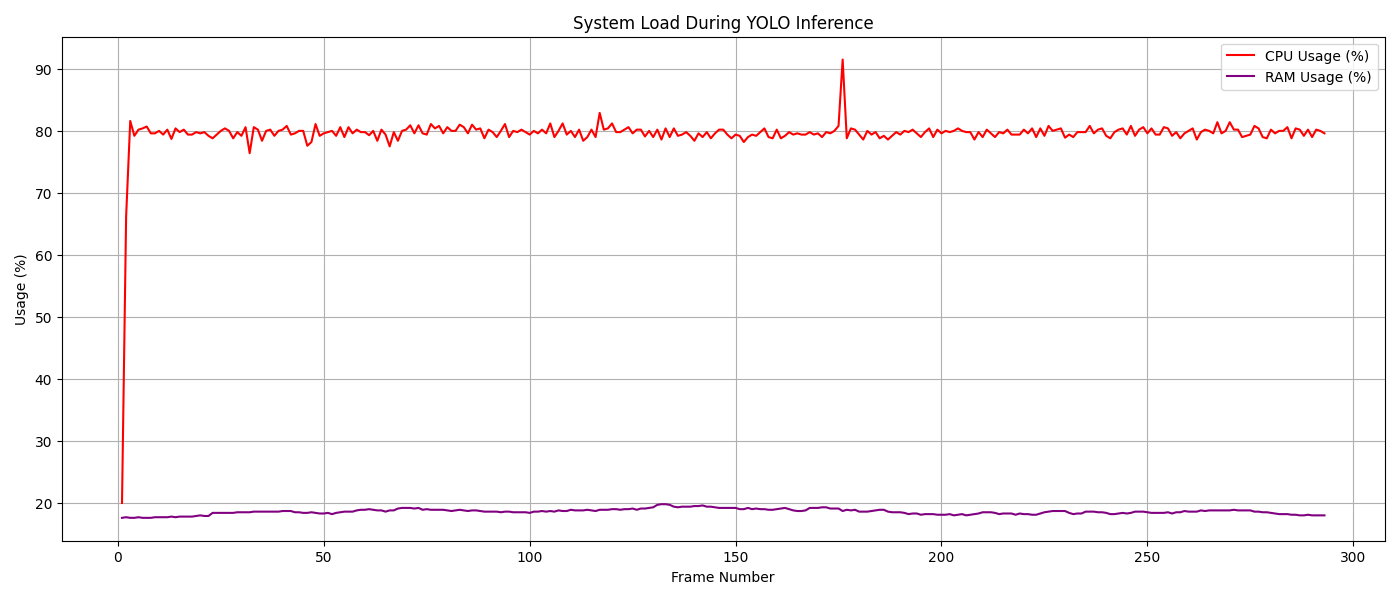
\includegraphics[width=\textwidth,height=5.9cm,keepaspectratio]{images/System_Load_During_Yolo_Inference.png}
    \caption{Systemauslastung während der Inferenz (RPI5)}
    \label{fig:CPU und RAM-Auslastung Inferenz RPI5}
  \end{subfigure}
  \hfill
  \begin{subfigure}[b]{\textwidth}
    \centering
    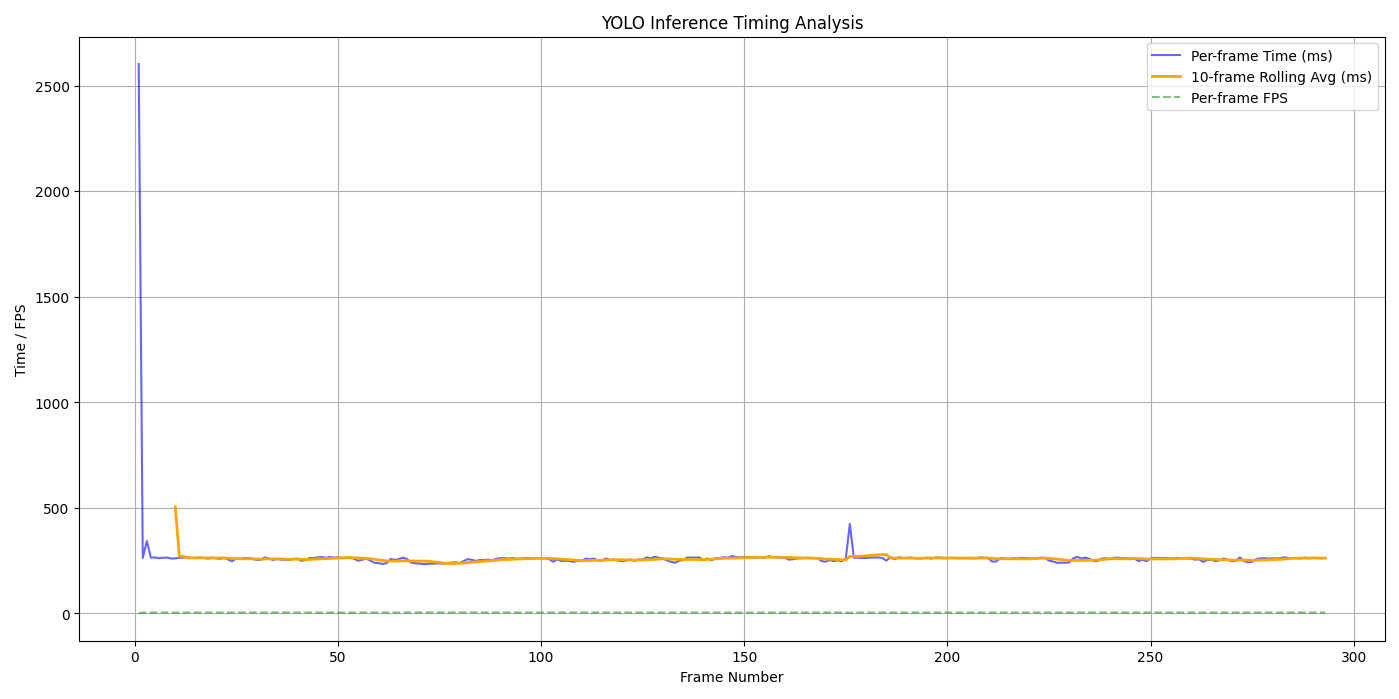
\includegraphics[width=\textwidth,height=6.2cm,keepaspectratio]{images/YOLO_Inference_Timing_Analysis.png}
    \caption{Zeitanalyse der Inferenz (RPI5)}
    \label{fig:Zeitanalyse der Inferenz (RPI5)}
  \end{subfigure}
  \caption{System- und Zeitanalyse während der Inferenz (RPI5)}
  \label{tab:System- und Zeitanalyse waehrend der Inferenz}
\end{figure}


\subsection{Inferenz des Modells auf dem Laborrechner (Jürgens)}
Mit dem Plattformwechsel wurde neben der Ausführungsumgebung ebenfalls das verwendete Modell geändert. So wurde das YOLOv8n Modell durch das YOLOv11 Modell ersetzt, welche hinsichtlich der Performance und Genauigkeit eine kleine Verbesserung bietet.
Die Inferenz des Modells auf dem Laborrechner erfolgt ebenfalls mit der Ultralytics Python-Bibliothek. Anders als auf dem RPI5 läuft die Berechnung des Modells auf der dedizierten Grafikkarte des Laborrechners. Hierbei handelt es sich um eine NVIDIA T1000 Grafikkarte welche die Nutzung von CUDA ermöglicht. Um dieses auch aktiv zu verwenden muss der \texttt{NVIDIA Cuda Compiler Driver} und PyTorch mit CUDA-Unterstützung installiert sein. Die Inferenzzeit des Modells auf dem Laborrechner fällt mit etwa 8 ms deutlich geringer aus und bietet eine flüssigere Anzeige des annotierten Kamera-Streams (siehe \ref{fig:Timing Zusammenfassung CUDA vs RPI5}). 
\begin{figure}[h]
  \centering
  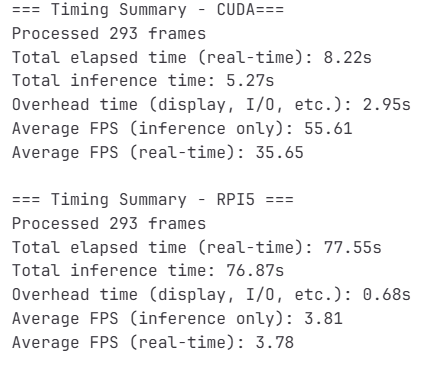
\includegraphics[scale=0.5]{images/Timing_summary.png}
  \caption{Timing Zusammenfassung CUDA vs RPI5}
  \label{fig:Timing Zusammenfassung CUDA vs RPI5}
\end{figure}
\newpage

Durch die Verwendung der dedizierten Grafikkarte wird nun anstelle der CPU die GPU für die Inferenz verwendet. Dies führt zu einer deutlich geringeren Belastung der CPU des Systems (siehe \ref{tab:CPU und RAM-Auslastung CPU vs CUDA})

\begin{figure}[h!]
  \centering
  \begin{subfigure}[b]{\textwidth}
    \centering
    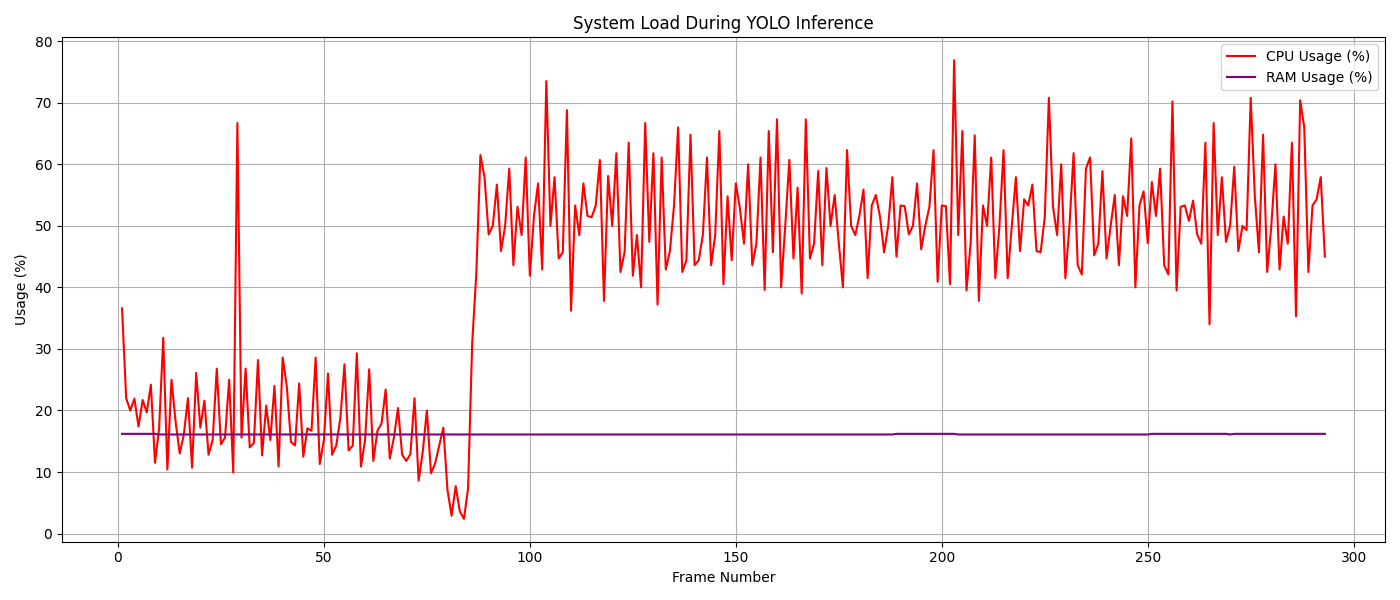
\includegraphics[width=0.9\textwidth,height=5.9cm,keepaspectratio]{images/system_load_plot_CPU_Laborrechner.png}
    \caption{Systemauslastung Laborrechner ohne CUDA}
    \label{fig:CPU und RAM-Auslastung ohne CUDA}
  \end{subfigure}
  \hfill
  \begin{subfigure}[b]{\textwidth}
    \centering
    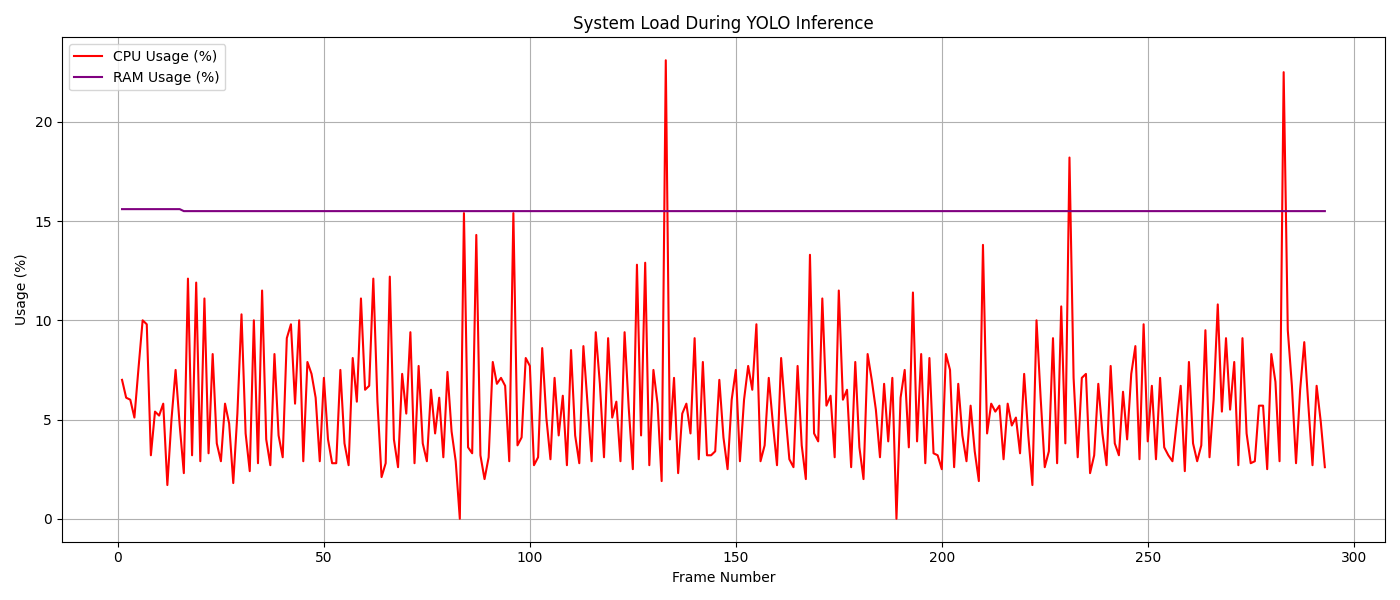
\includegraphics[width=0.9\textwidth,height=6.2cm,keepaspectratio]{images/system_load_plot_CUDA.png}
    \caption{Systemauslastung Laborrechner mit CUDA}
    \label{fig:CPU und RAM-Auslastung mit CUDA}
  \end{subfigure}
  \caption{Vergleich Inferenz ONNX C++ und Python}
  \label{tab:CPU und RAM-Auslastung CPU vs CUDA}
\end{figure}

\newpage

Der Rückgabewert der Inferenz des Modells beinhaltet unter anderem die Koordinaten der Bounding Box, die Klasse und den Konfidenzwert des erkannten Objekts. Die Konfidenz gibt an, zu wie viel Prozent sich das Modell bei dem erkannten Objekt sicher ist. \cite{InferenzResults} 

Diese Informationen können nun direkt für weitere Aktionen verwendet werden. Die detektierte Bounding Box wird dem Frame des Kamera-Streams hinzugefügt und auf dem Bildschirm angezeigt. 
\chapter{Einrichtung einer Ultra-Low-Latency Videoübertragung \label{sec:webrtc}}
\section{Anforderungen an die Videoübertragung (Jürgens)}
Die angebundene Kamera des RPi5 soll zukünftig neben dem Stream für die KI-Auswertung auch das 'Auge' des Roboters darstellen. So soll die Sicht des Roboters in nahezu Echtzeit abrufbar sein. Daher muss neben einer robusten Verbindung besonders auch die Latenz der Videoübertragung so gering wie möglich gehalten werden. Die bisherige Implementation mittels einer libcamera-Pipeline als Sender und einer GStreamer-Pipeline als Empfänger ist mit einer Latenz von etwa 1 Sekunde nicht für die Echtzeitübertragung geeignet. Nach einer Recherche zu verschiedenen Streaming-Protokollen und -Techniken wurde die Entscheidung getroffen, dass zukünftig eine Lösung mittels WebRTC verwendet werden soll. WebRTC bietet eine Lösung mit einer Latenz von unter 500 ms an, welches für dieses Projekt mehr als ausreichend ist \cite{WebRTCLatency}.

\section{Grundlegende Informationen zu WebRTC (Jürgens)}
WebRTC ist ein freies, offenes Softwareprojekt welches eine Lösung für die Echtzeitkommunikation von Browsern und mobilen Anwendungen bietet. Mittels einer Peer-To-Peer Verbindung können unter Anderem Audio- und Videodaten in Echtzeit zwischen den Peers übertragen werden. Dieses Vorgehen ermöglicht eine direkte Kommunikation zwischen den Peers ohne einen zentralen Server, was zu einer geringeren Latenz führt.
Bei dem Verbindungsaufbau wirken verschiedene Komponenten und Protokolle zusammen, um eine stabile und sichere Verbindung zwischen den Peers herzustellen. Ein wichtiger Bestandteil von WebRTC ist der Signalisierungsprozess. Dieser ist für den Austausch von Metadaten zwischen den Peers verantwortlich. \cite{WebRTCBasics}

\section{Herstellung der WebRTC-Verbindung (Jürgens)}
Insgesamt wurden zwei Ansätze bei der Herstellung der WebRTC-Verbindung zwischen dem RPI5 und dem Laborrechner verfolgt. Der erste Ansatz war der direkte Aufbau einer Peer-To-Peer Verbindung.
Mit der Python-Bibliothek \texttt{aiortc} konnte eine WebRTC-Verbindung hergestellt werden. Mittels GStreamer und OpenCV wird diese Verbindung mit dem Kamerabild angereichert und an den Empfänger gesendet. Durch das Hinzufügen eines Keep-Alives-Kanal wird sichergestellt, dass die Verbindung zwischen den Peers beibehalten wird und nicht nach einer gewissen Zeit abbricht. Mit diesem Ansatz konnte eine stabile Verbindung mit geringer Latenz zwischen dem RPi5 und dem Laborrechner hergstellt werden.

Durch weitere Absprachen mit dem Team kam der Wunsch auf, dass die Videoübertragung nicht nur einzig und allein für die KI-Auswertung genutzt werden soll, sondern auch aus dem LAN über eine Website aufrufbar sein soll. Mit dieser Anforderung wurde der zweite Ansatz verfolgt, welcher den Einsatz eines MediaMTX-Servers beinhaltet. MediaMTX ist ein Open-Source Media-Server welcher eine Vielzahl von Protokollen unterstützt, darunter auch WebRTC. Der MediaMTX-Server wird dabei auf dem RPI5 installiert und ausgeführt. Die Konfiguration der Servers erfolt über eine YML-Datei.
In dieser können beispielsweise Ports und Protokolle festgelegt werden. Neben der grundlegenden Konfiguration kann hier auch das Startverhalten des Servers festgelegt werden. So wird beim Start automatisch ein Libcamera-Stream an den Server mittels RTSP übergeben. Über den Standardport 8889 kann der Stream schlussendlich über WebRTC mittels Browser abgerufen werden. Um den WebRTC-Stream auch außerhalb einer Browser-Umgebung abrufen zu können, bietet MediaMTX eine WHEP-Schnittstelle an. Über diese WHEP-Schnittstelle kann der Stream beispielsweise in anderen Anwendungen abgerufen werden. Diese Schnittstelle ermöglicht es, den Stream in unserem Python-Script zu verwenden und die KI-Auswertung auf dem Stream durchzuführen. 

Mit dieser Implementation ist es möglich die KI-Auswertung auf einem Ultra-Low-Latency Stream anzuwenden und so in nahezu Echtzeit die Objekterkennung durchzuführen während der Kamerastream von anderen Geräten aus dem LAN per Browser angeschaut werden kann. In der Abbildung \ref{fig:KI-webRTC-Architektur} ist die Architektur des WebRTC-Streams in Zusammenarbeit mit der KI-Auswertung noch einmal dargestellt. 

\begin{figure}[H]
  \centering
  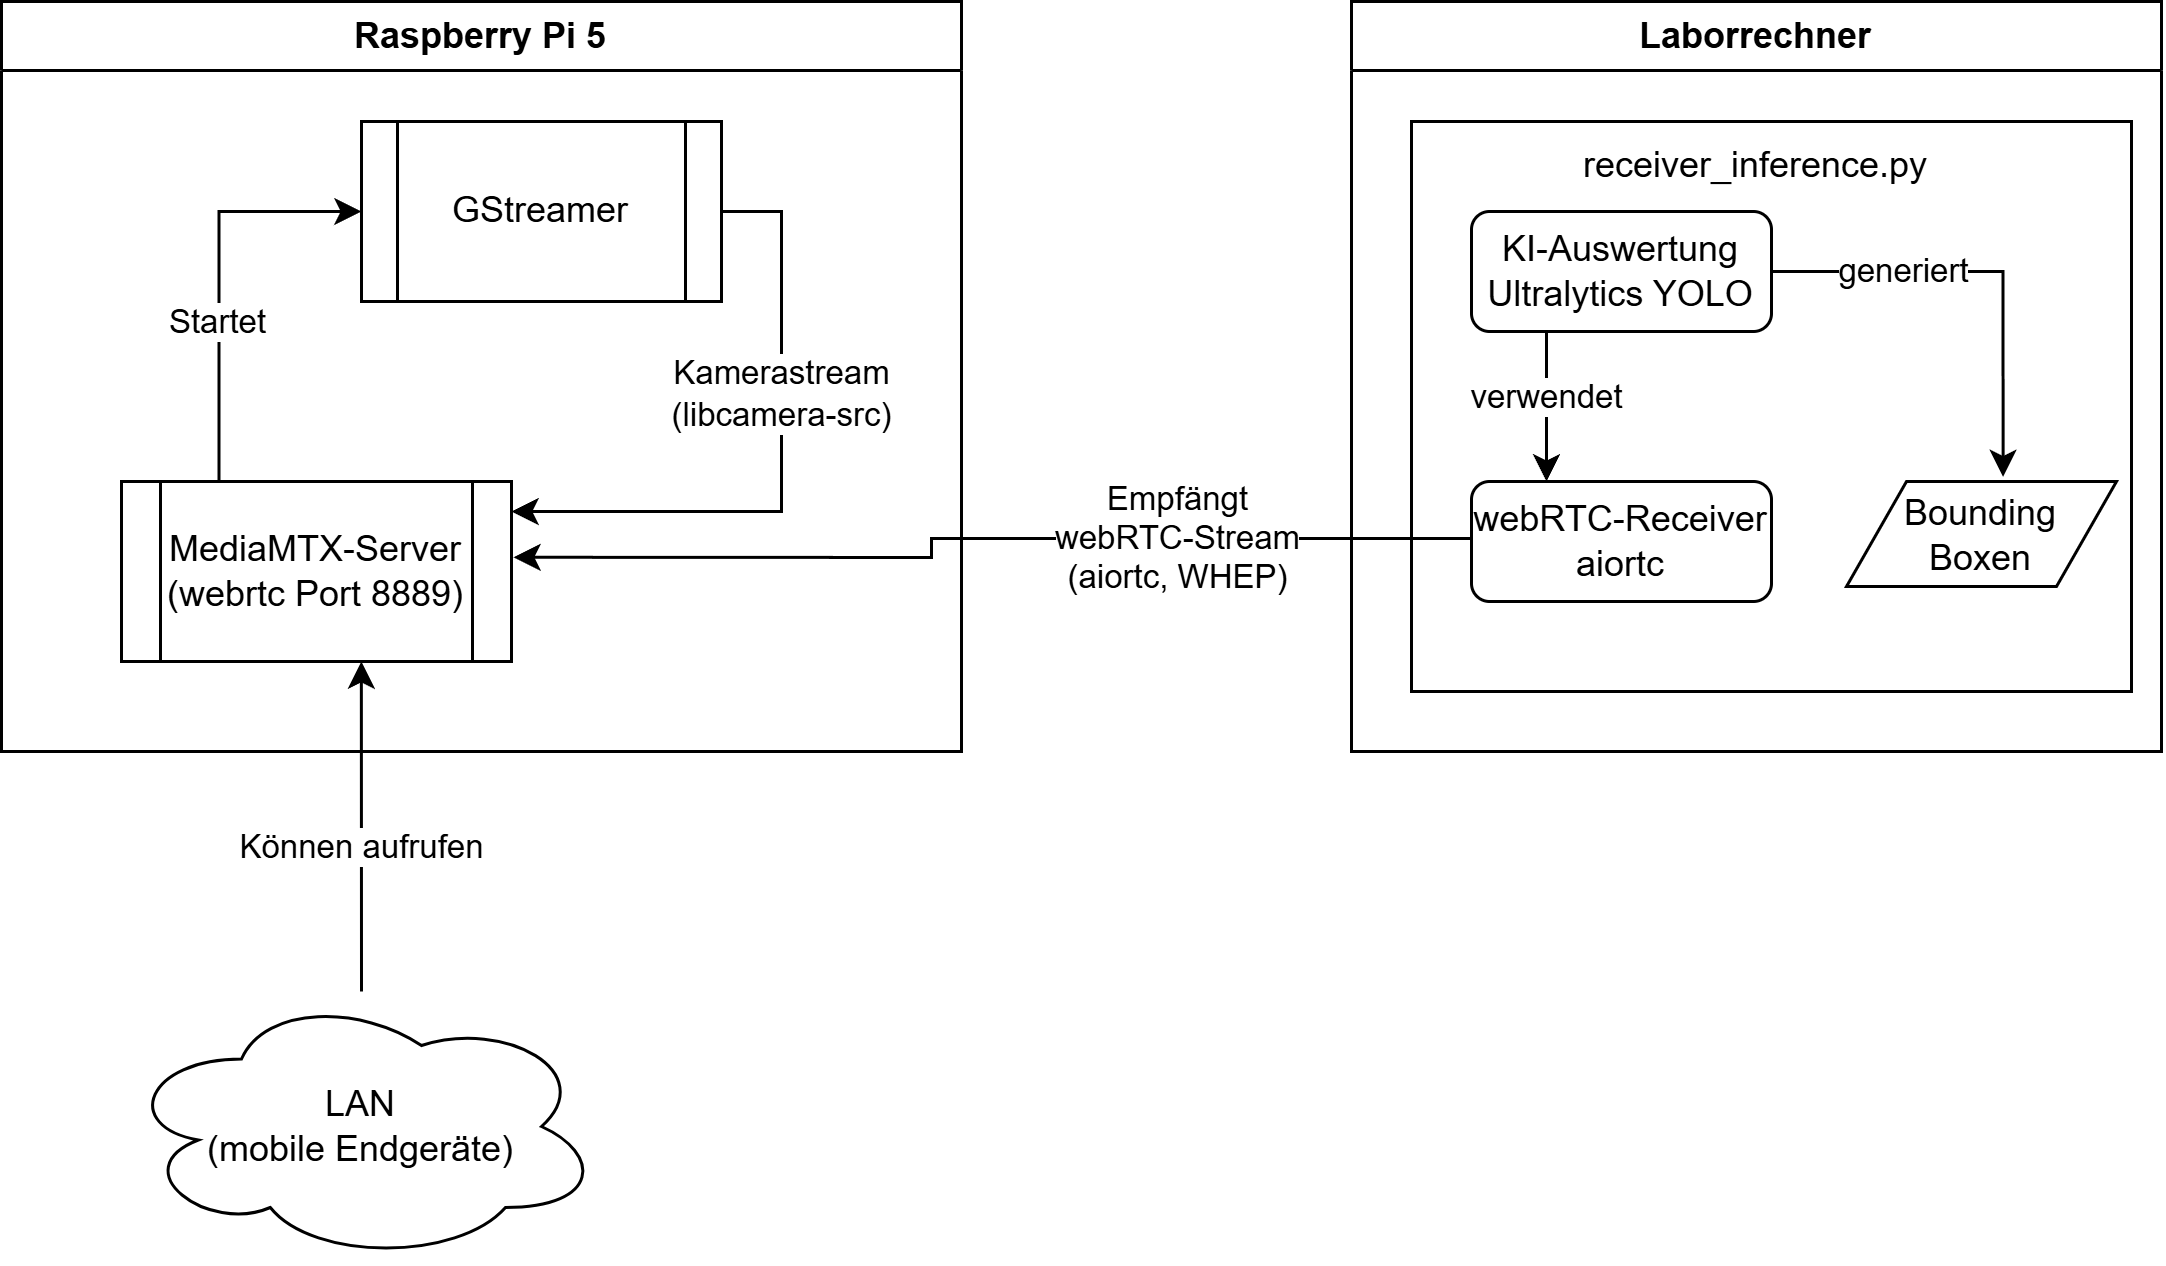
\includegraphics[width=0.95\textwidth]{images/ki-webrtc-arch.png}
  \caption{Architekturübersicht: Zusammenspiel von KI-Modell und WebRTC-Streaming}
  \label{fig:KI-webRTC-Architektur}
\end{figure}

\chapter{Objekttracking (Jürgens)}
\section{Ziel des Objekttrackings (Jürgens, Specht)}
Eine optionale Anforderung die in diesem Projekt am Ende noch aktiv verfolgt und umgesetzt wurde, war die Implementierung eines Objekttrackings. So sollte es möglich sein, die Koordinaten der Bounding Box zur Steuerung des Geschützarms zu verwenden. Das Ziel war also, den Geschützarm immer so auszurichten, dass die Bounding Box des Objekts immer in der Mitte des Kamerabildes ist. 

\section{Einrichtung des Kommunikationskanals (Jürgens)}
Um tatsächlich Steuersignale an den Roboter zu senden, muss zunächst entschieden werden, wie dies geschehen soll. Dabei gab es zwei Ansätze die in Betracht gezogen wurden: 
\begin{itemize}
    \item Kommunikation über WebSockets
    \item Kommunikation über MQTT
\end{itemize}
Nach Absprachen mit dem Team wurde entschieden, dass die Kommunikation über MQTT erfolgen soll. Dies hat den Vorteil, dass mittels eines MQTT-Brokers eine zentrale Stelle geschaffen wird, an dem alle Nachricht gesammelt werden können. Dies ermöglicht neben dem grundlegend einfachen Austausch von Nachrichten auch eine gute Möglichkeit um das Projekt zu erweitern. So können weitere Sensorwerte oder auch die Stellung der Motoren über den MQTT-Broker ausgetauscht werden und optional für weitere Aktionen verwendet werden. Es wurde sich auf die Lösung mit dem Open-Source MQTT-Broker \texttt{Mosquitto} geeinigt. Dieser MQTT-Broker stellt eine leichtgewichtige Lösung bereit, welche nach dem Publish-Subscribe-Prinzip arbeitet \cite{Mosquitto}. So kann jeder Subscriber (Abonnent) ein oder mehrere Topics (Themen) abonnieren und erhält über diese dann Nachrichten. Dieser Ansatz soll den Nachrichtenverkehr für den Microcontroller minimieren, da hier zuvor bereits selektiert wird, welche Topics abonniert werden. 
\\ 
Die Mosquitto-Instanz wird auf dem Laborrechner installiert und ausgeführt. Die Konfiguration erfolgt über eine zentrale Konfigurationsdatei. Trotz korrekter Konfiguration konnte zunächst keine Verbindung zwischen dem MQTT-Broker und dem ESP32 hergestellt werden. Dieser Umstand wurde durch Ergänzung von Firewall-Regeln auf dem Laborrechner behoben. Es wurde auf dem Windows Rechner explizit eine eingehende und ausgehende Regel für Mosquitto erstellt. So konnte erfolgreich eine Verbindung zwischen dem ESP32 und dem MQTT-Broker hergestellt werden.

\section{Implementierung des Objekttrackings (Jürgens, Specht)}
Mit bestehender und funktionierender MQTT-Verbindung konnte nun das Objekttracking implementiert werden. Dabei musste besonders auf die Art und Weise geachtet werden, wie die Motorsteuerung implementiert wurde. Die Motoren werden mit Statusnachrichten versorgt, welche die absolute Position der Motoren angeben. So würde das Senden mehrere Nachrichten mit dem selben Inhalt zu einer einzigen Bewegung führen. Somit sind die Nachrichten idempotent und können mehrfach gesendet werden, ohne dass sich die Position der Motoren ändert.
Wichtig war außerdem, dass die Berechnung der Drehwinkel auf dem Laborrechner erfolgt. Hiermit soll der ESP32 entlastet werden, da dieser nur als Abonnent des MQTT-Topics fungiert und die Motoren steuert. 
\\
Mit diesem Wissen wurde zunächst der Ansatz eines Mappings verfolgt. Dabei wurde der Geschützarm in die Null-Stellung gebracht. Durch Trial-and-Error wurden dabei die maximal benötigten Drehwinkel der Motoren die benötigt werden um die Kamera an den Bildrand zu bewegen, ermittelt. Diese Werte wurden dann in ein Mapping überführt. So sollte sich das errechnete Zentrum der Bounding Box in einen benötigten Drehwinkel übersetzen lassen.\\
Dieses Vorgehen hat sich jedoch als nicht praktikabel herausgestellt. So wurden beispielsweise für das Erreichen des rechten Bildrandes eine andere Motorstellung benötigt als für das Erreichen des linken Bildrandes. So wurde beispielsweise für das Erreichen des rechten Bildrandes der horizontale Winkel auf -15 gesetzt, für das Erreichen des linken Bildrandes jedoch +18. Aufgrund dieser Abweichungen und einem inkosistenten Verhalten der Motoren wurde der Ansatz verworfen und nicht weiter verfolgt.
\\
Der zweite Ansatz wurde gemeinsam mit Michael Specht erarbeitet und verfolgt die Idee, die Kameramerkmale direkt mit in die Berechnung des Drehwinkels einzubeziehen. Dieser Ansatz erwies sich als deutlich erfolgreicher hatte dabei aber auch eine höhere Komplexität. %Dabei wurde zunächst die Seitenverhältnisse ermittelt. Diese wurden aus der Breite und Höhe des Kamerabildes ermittelt. Diese liegen bei 1280 Pixeln in der Breite und 1080 Pixel in der Höhe. Daraus ergibt sich das Seitenverhältnis (Aspect Ratio) des Kamerabildes:

%\begin{equation}
%    \text{Aspect\_ratio} = \frac{\text{Bildbreite}}{\text{Bildhöhe}} = \frac%{1280}{1080} = 1{,}185
%\end{equation}
%
%Anhand des Datenblattes der Kamera wurde die diagonale Sichtweite (diagonal %fov) ermittelt. Diese beträgt bei dem Raspberry Camera Module 3 75 Grad \cite%{raspberrypi5cammodule3}. Für eine korrekte Berechnung der Drehwinkel ist eine %Umrechnung in Radiant notwendig. Die Python Bibliothek \texttt{math} stellt %dafür die Funktion \texttt{radians()} bereit.


 % Ich habe keine Ahnung was Claude da im Code gemacht hat, vielleicht hast du ja eine Ahnung? Ich hab es mit Winkeln nicht so :D 

\chapter{Webserver (Koch)}
\label{sec:Webserver}
\section{Funktion und Anforderung des Webservers}
Der Webserver des Projekts sollte die zentrale Schnittstelle zwischen verschiedenen Sensoren werden und sowohl Videomaterial mit bereits verarbeiteten KI-Informationen darstellen können und wissenswerte Daten wie die Entfernung des Fliegers oder die Geschützneigung anzeigen.
Als zentrales Problem stand dabei das Videomaterial mit entsprechenden Bounding Boxes anzuzeigen im Vordergrund, da bereits über das ganze Projekt hinweg die KI die leistungsintensivste Aufgabe war und entsprechende Latenzprobleme bereits auf das Minimum verringert wurden.
Der Grundlegende Aufbau der KI-Verarbeitung mitsamt der Videoausgabe ist in \ref{JENDRIK} erklärt.

\section{Lösungsansatz und Umsetzung}
Ein Lösungsansatz diesbezüglich war deshalb, dass die Sensordaten vom Raspberry Pi per MQTT an den PC geschickt werden, welcher die KI-Verarbeitung übernimmt, um die Daten direkt im Videostream abzubilden.
Das Video mit den Bounding Boxes und den Sensordaten sollte dann zurück auf den MediaMTX-Server geschickt werden, worüber man dann das Video sehen kann.
Dieser Ansatz war allerdings keine geeignete Lösung, da die Verarbeitung zu lange dauerte und somit eine zu geringe Framerate erreicht wurde, wodurch dies keine annehmbare Lösung darstellte.


Deshalb wurde der alternative Ansatz gewählt, dass der Raspberry Pi selbst den Webserver bereitstellt, da dieser bereits die Sensordaten und den MediaMTX-Server bereitstellt.
Das Problem hierbei war jedoch, dass somit zwar der Videostream und die Sensordaten dargestellt werden konnten, allerdings noch keine Bounding Boxes, welche eine harte Anforderung an den Webserver waren.
Es musste also eine Lösung gefunden werden, den verarbeiteten Videostream mit den Bounding Boxes vom PC zum Raspberry Pi zu übertragen, doch das senden des Videostreams ist nicht ohne Verluste möglich, wie bereits erwähnt wurde.

Die Umsetzung erfolgte über einen zentralen Knotenpunkt auf dem Raspberry Pi, welcher sowohl die Bereitstellung der Benutzeroberfläche als auch die Echtzeitkommunikation mit den Sensoren und der externen KI-Komponente zur Objekterkennung übernimmt. Die Kommunikation erfolgt über WebSockets, wobei sowohl Sensordaten als auch Bounding-Box-Koordinaten empfangen, verarbeitet und an das Frontend weitergeleitet werden. Die Darstellung im Browser kombiniert dabei Livevideo, Sensordaten und erkannte Objekte in einem einheitlichen Interface. 
Dabei wird die Entfernung nur in Kombination mit der Bounding Box ausgegeben wie in Abbildung \ref{fig:webserver} zu sehen.
Während der Entwicklung zeigte sich, dass die zunächst gewählte Architektur zur Sensoranbindung zu erheblichen Verzögerungen führte. Die ursprüngliche Implementierung versuchte, beide Sensoren (Gyrosensor und Ultraschallsensor) über asynchrone Generatoren auszulesen, jedoch geschah dies nur sequentiell. Vermutlich bremste dabei die Verarbeitung des Ultraschallsensors, der mit geringerer Frequenz Daten liefert, die Verarbeitung des Gyrosensors aus. In der Folge wurden die Gyroskopdaten gepuffert und verzögert ausgegeben.
Um dieses Problem zu beheben, wurde die Architektur angepasst und die Sensorverarbeitung parallelisiert. Statt beide Generatoren sequentiell abzufragen, wurden zwei Tasks erstellt, die jeweils eigenständig mit ihrem Sensor kommunizieren. Dadurch können beide Datenströme unabhängig voneinander verarbeitet und weitergeleitet werden, was die Reaktionszeit des Systems verbesserte und die gleichzeitige Darstellung der Sensorinformationen im Frontend ermöglichte.
\begin{figure}[H]
    \begin{center}
        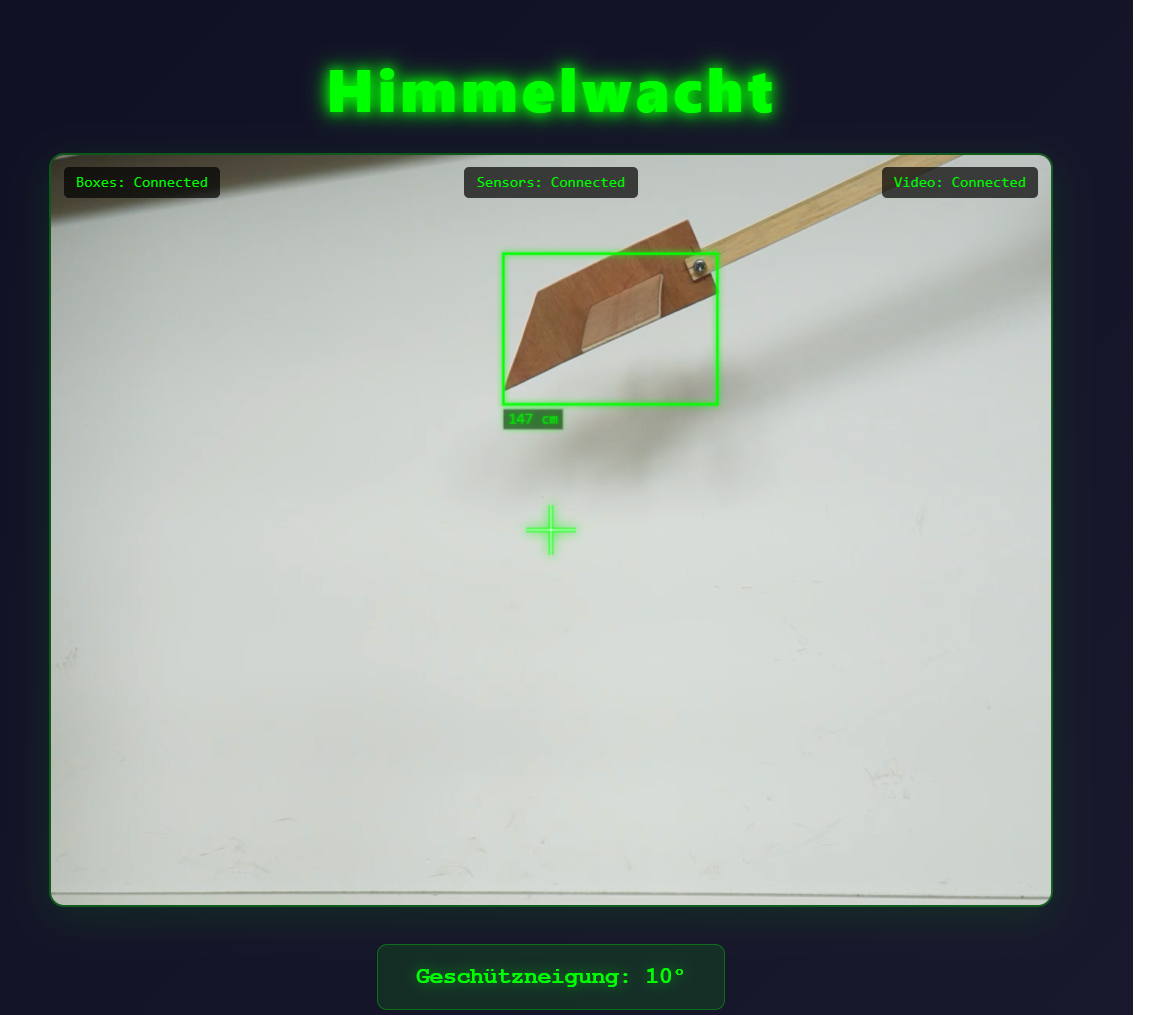
\includegraphics[width=0.8\textwidth]{images/Webserver.png}
        \caption{Webinterface zur Darstellung des Videostreams mit Bounding Boxes und Sensordaten}
        \label{fig:webserver}
    \end{center}
\end{figure}
%\input{gnn}
%\input{p5p}
%\input{end.tex}

% Time tables
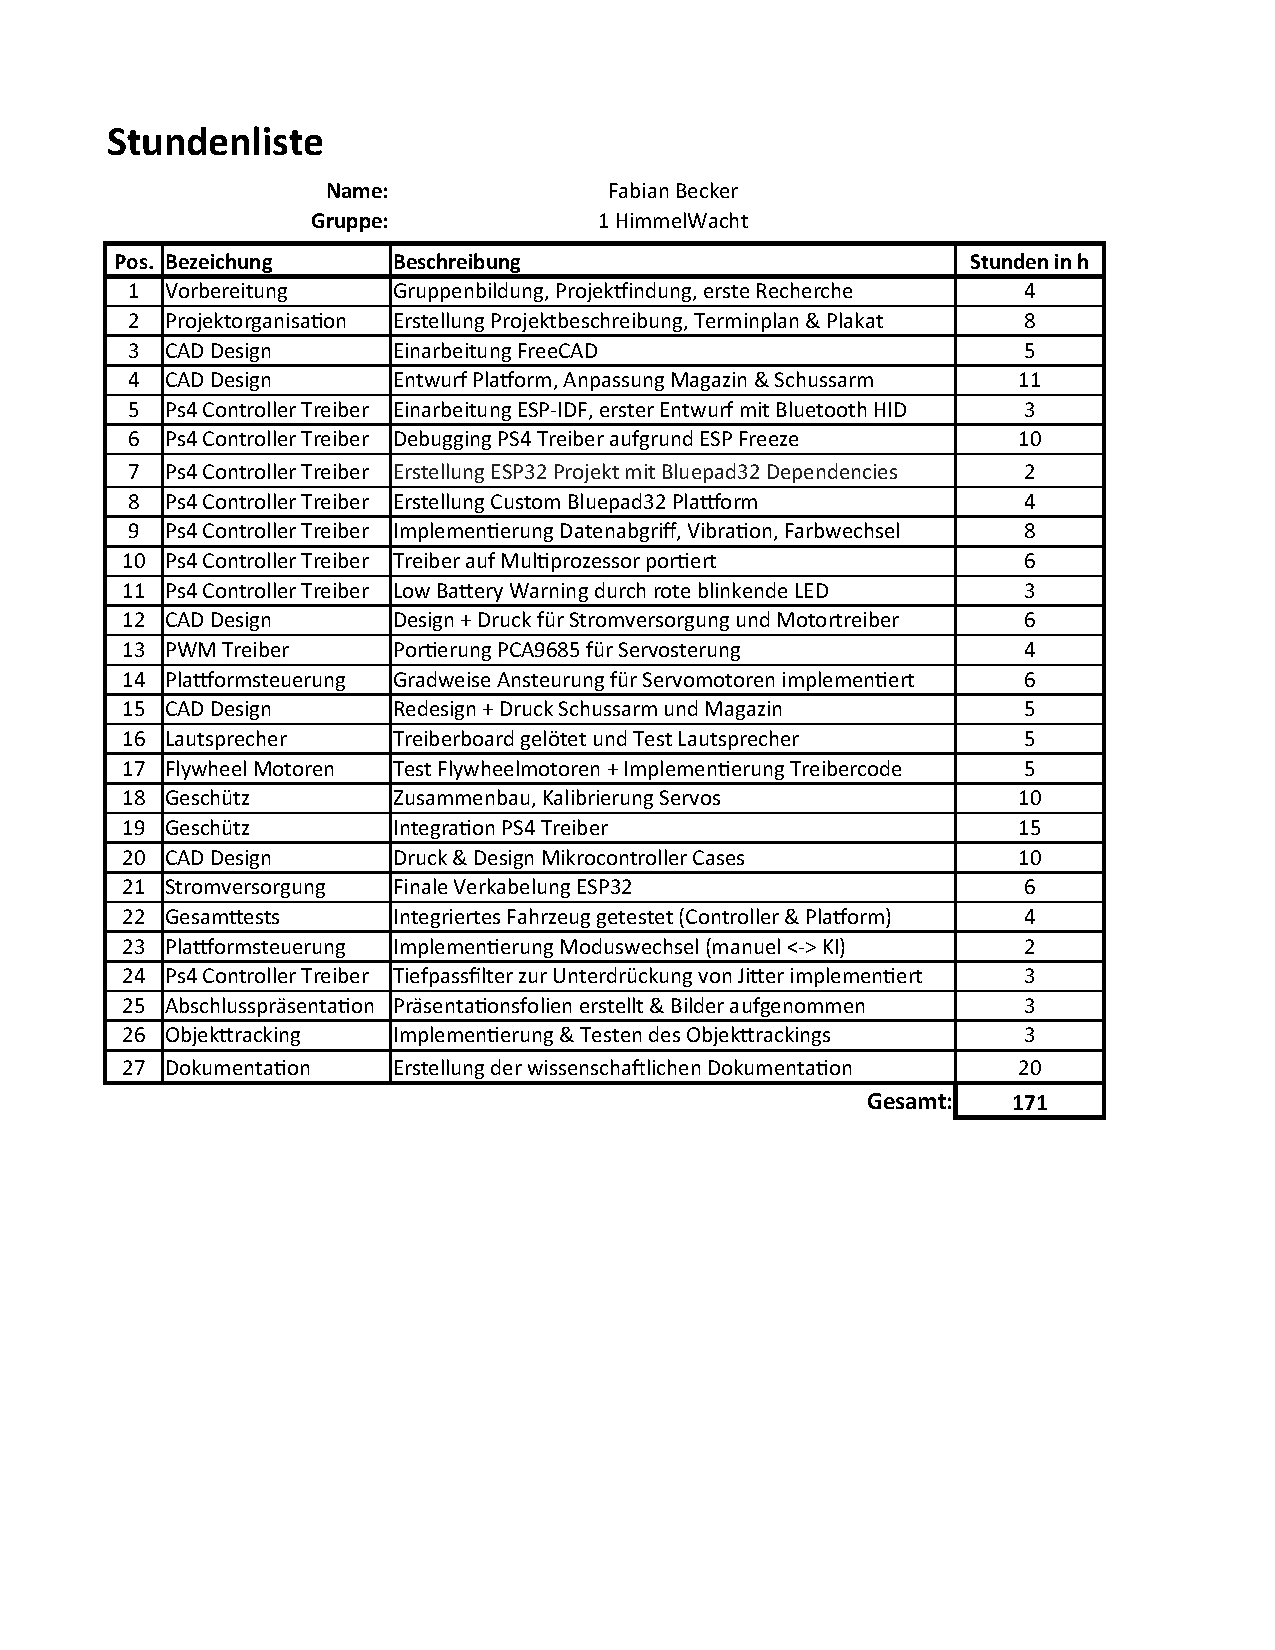
\includepdf[pages=-]{pdfs/Stundenliste_Fabian_Becker.pdf}
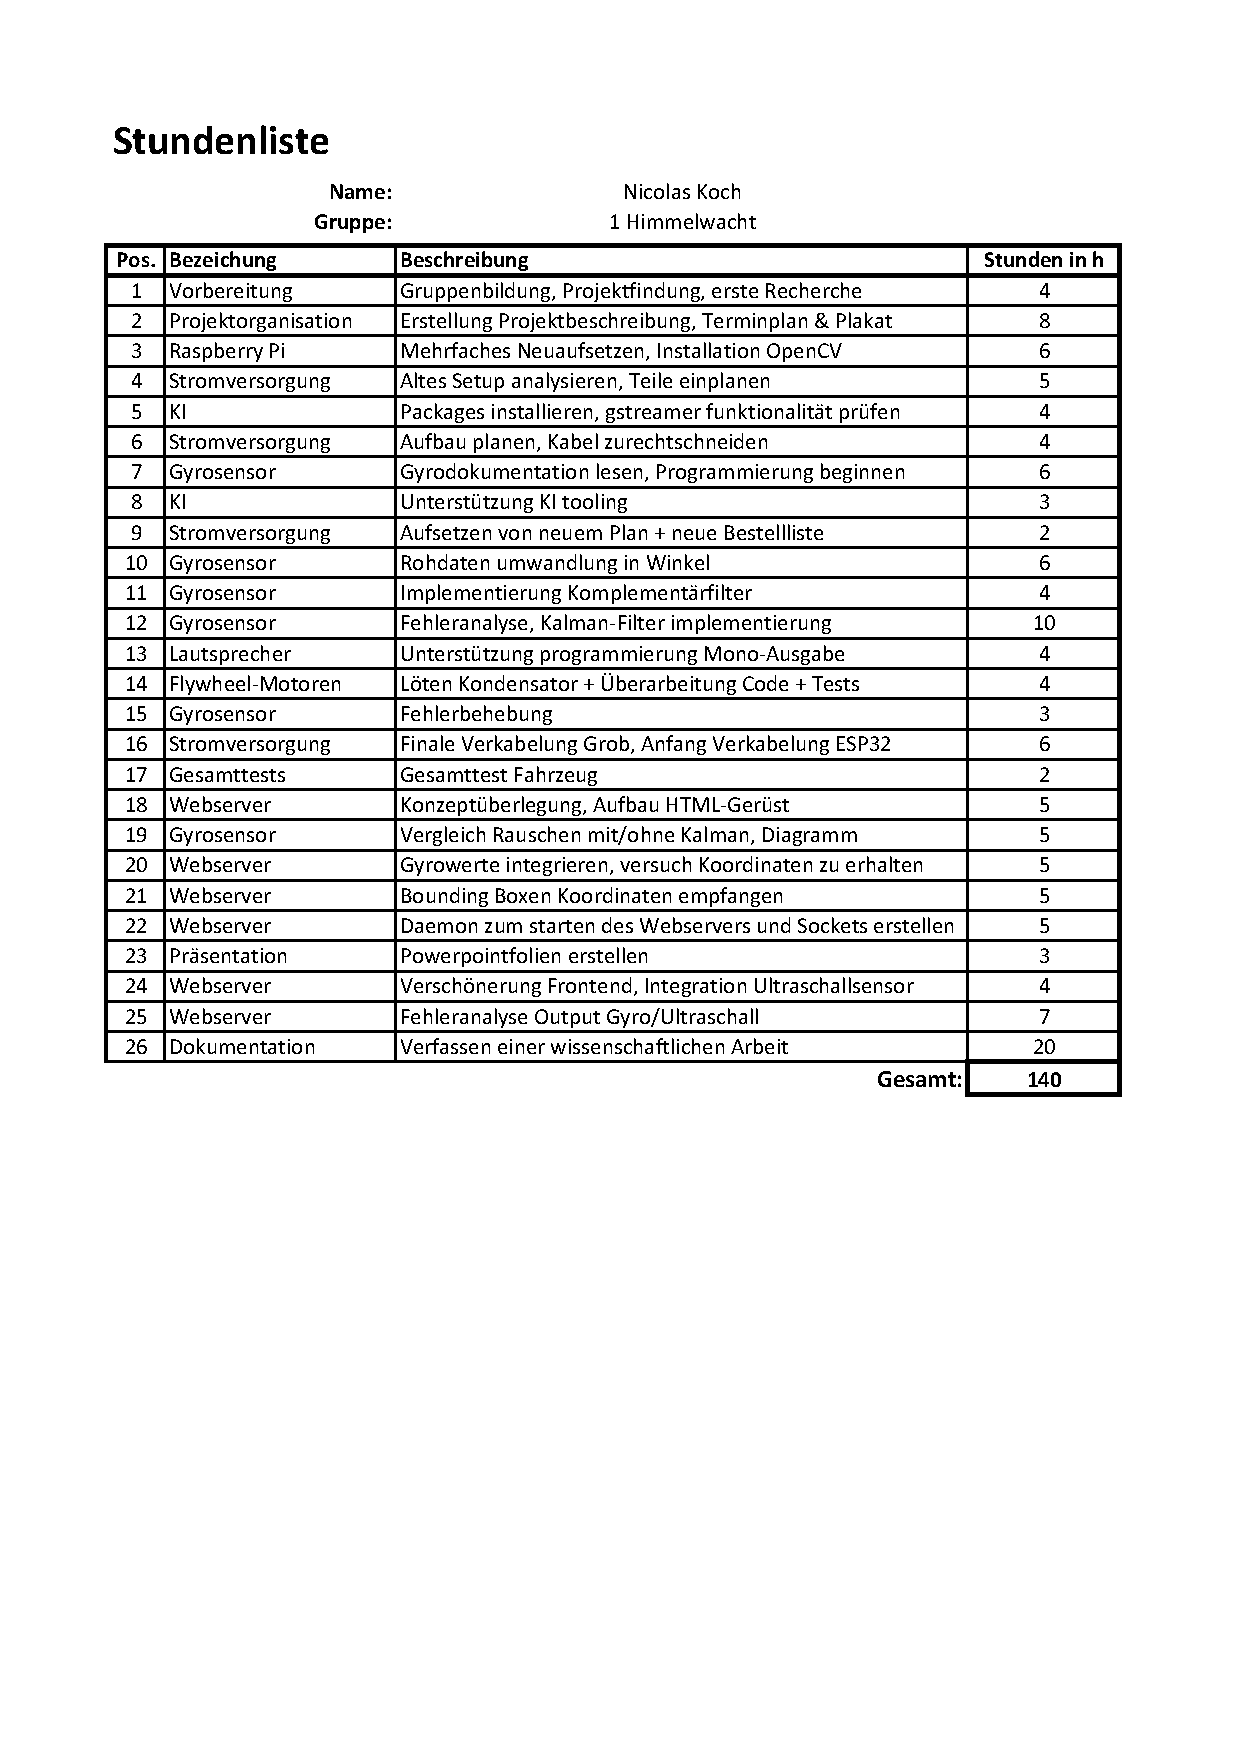
\includepdf[pages=-]{pdfs/Stundenliste_Nicolas_Koch.pdf}
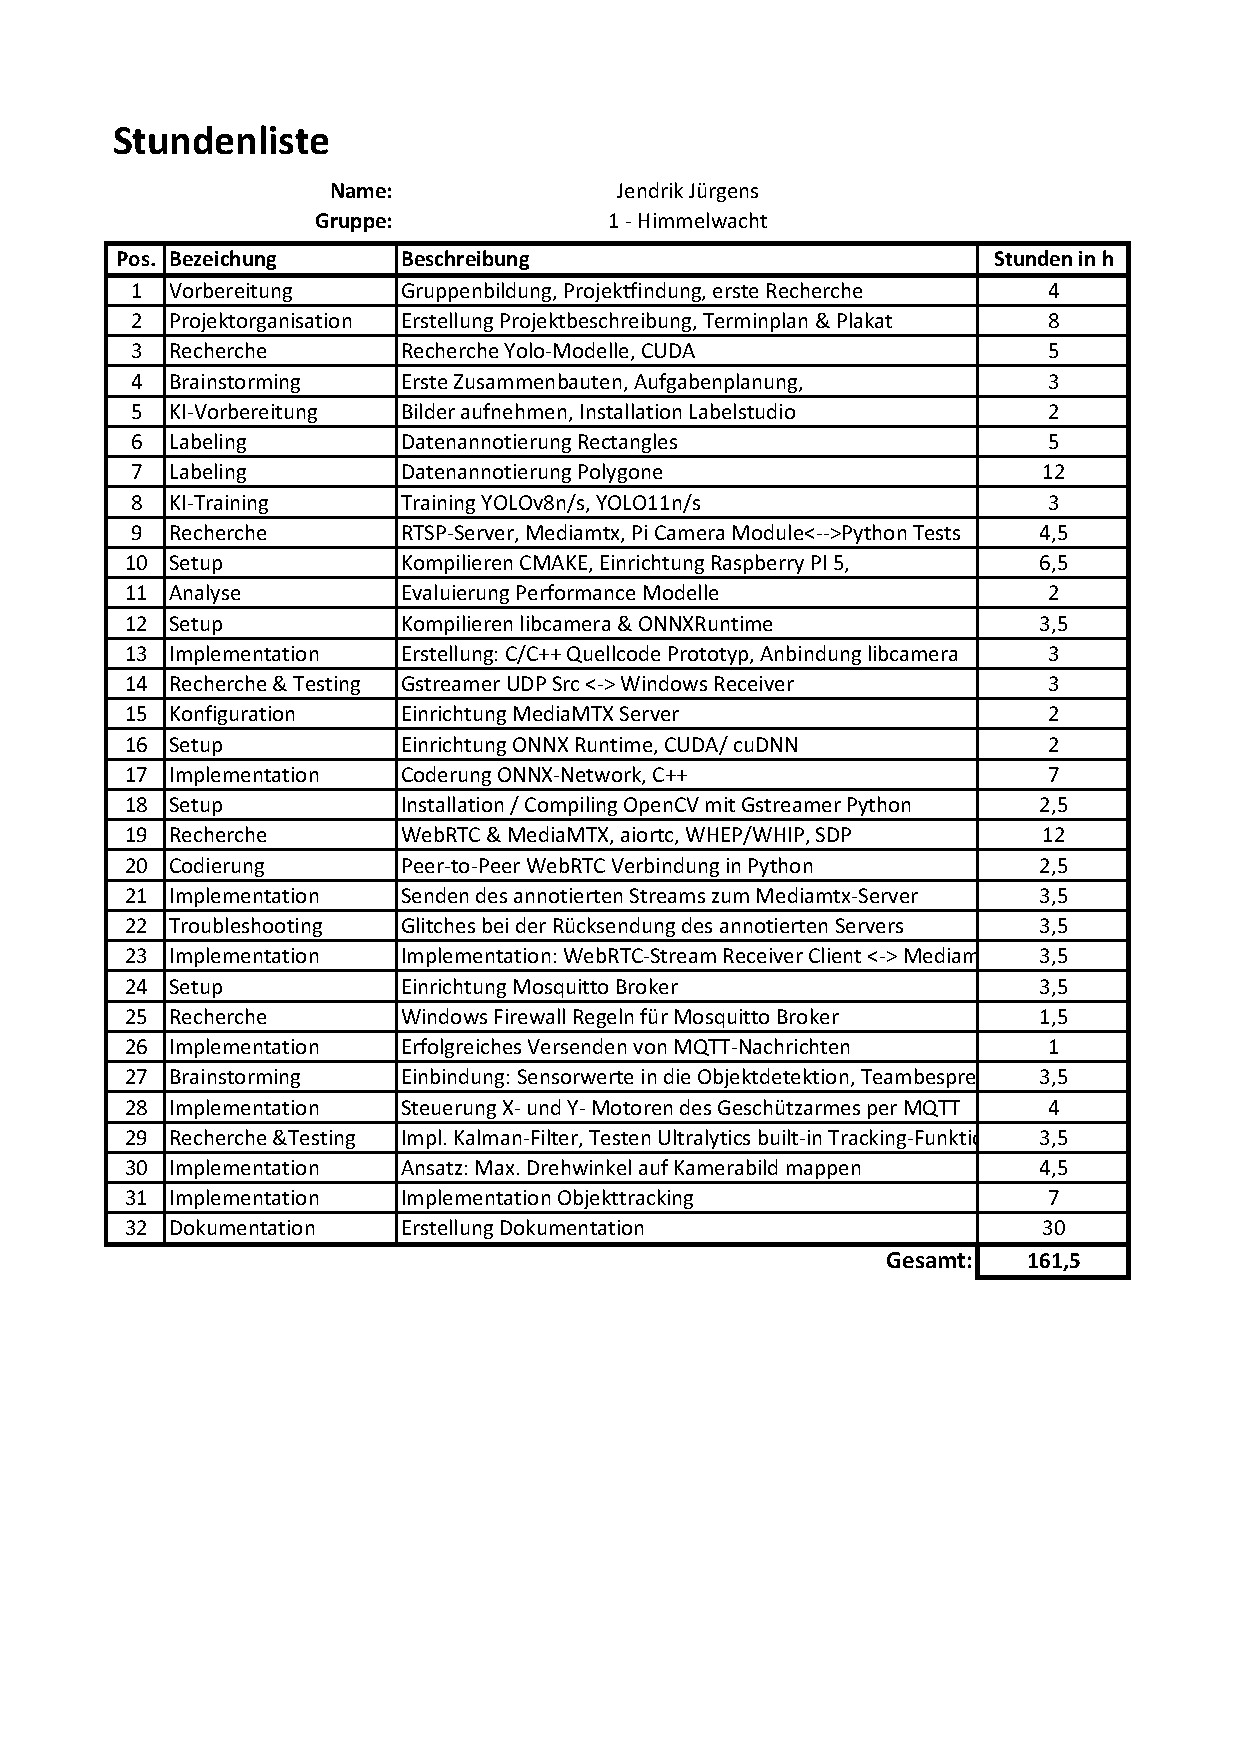
\includepdf[pages=-]{pdfs/Stundenliste_Jendrik_Juergens.pdf}
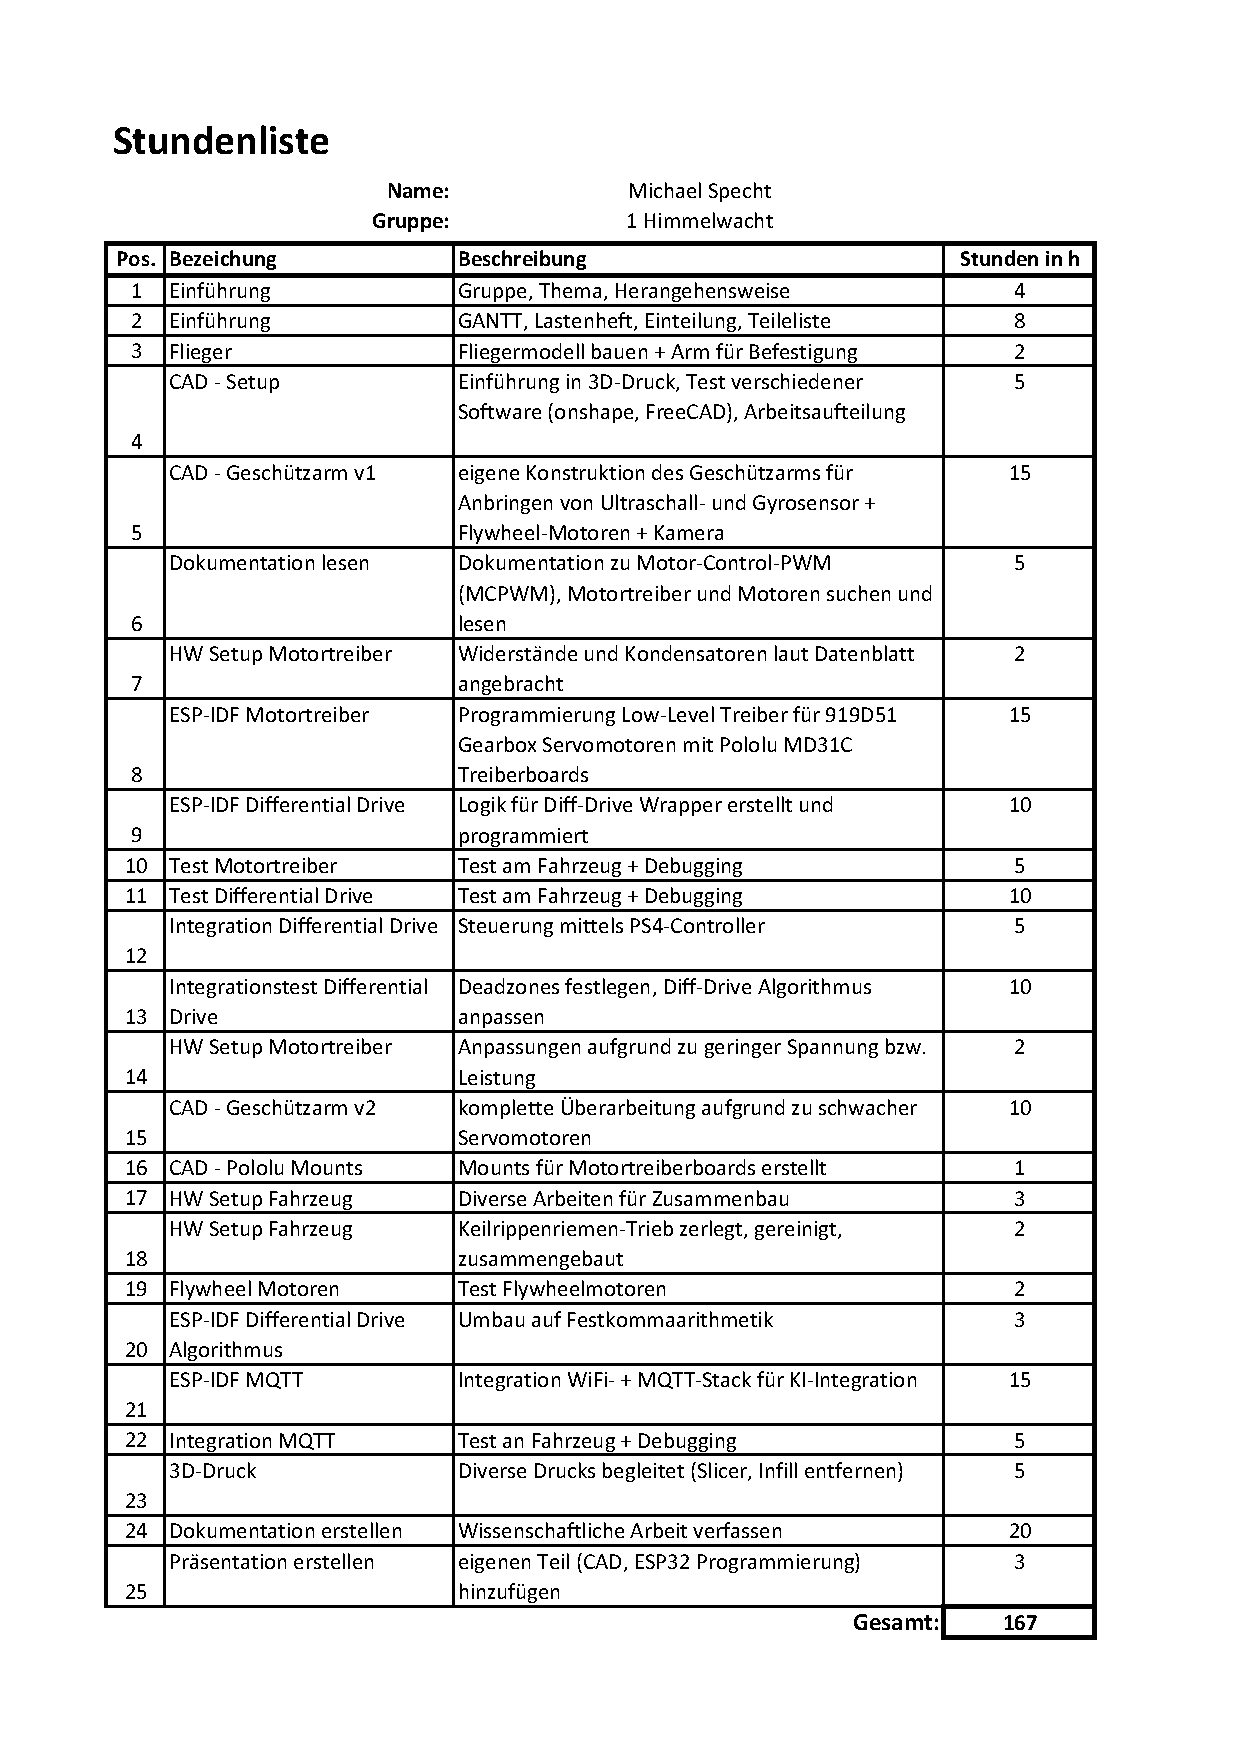
\includepdf[pages=-]{pdfs/Stundenliste_Michael_Specht.pdf}
% 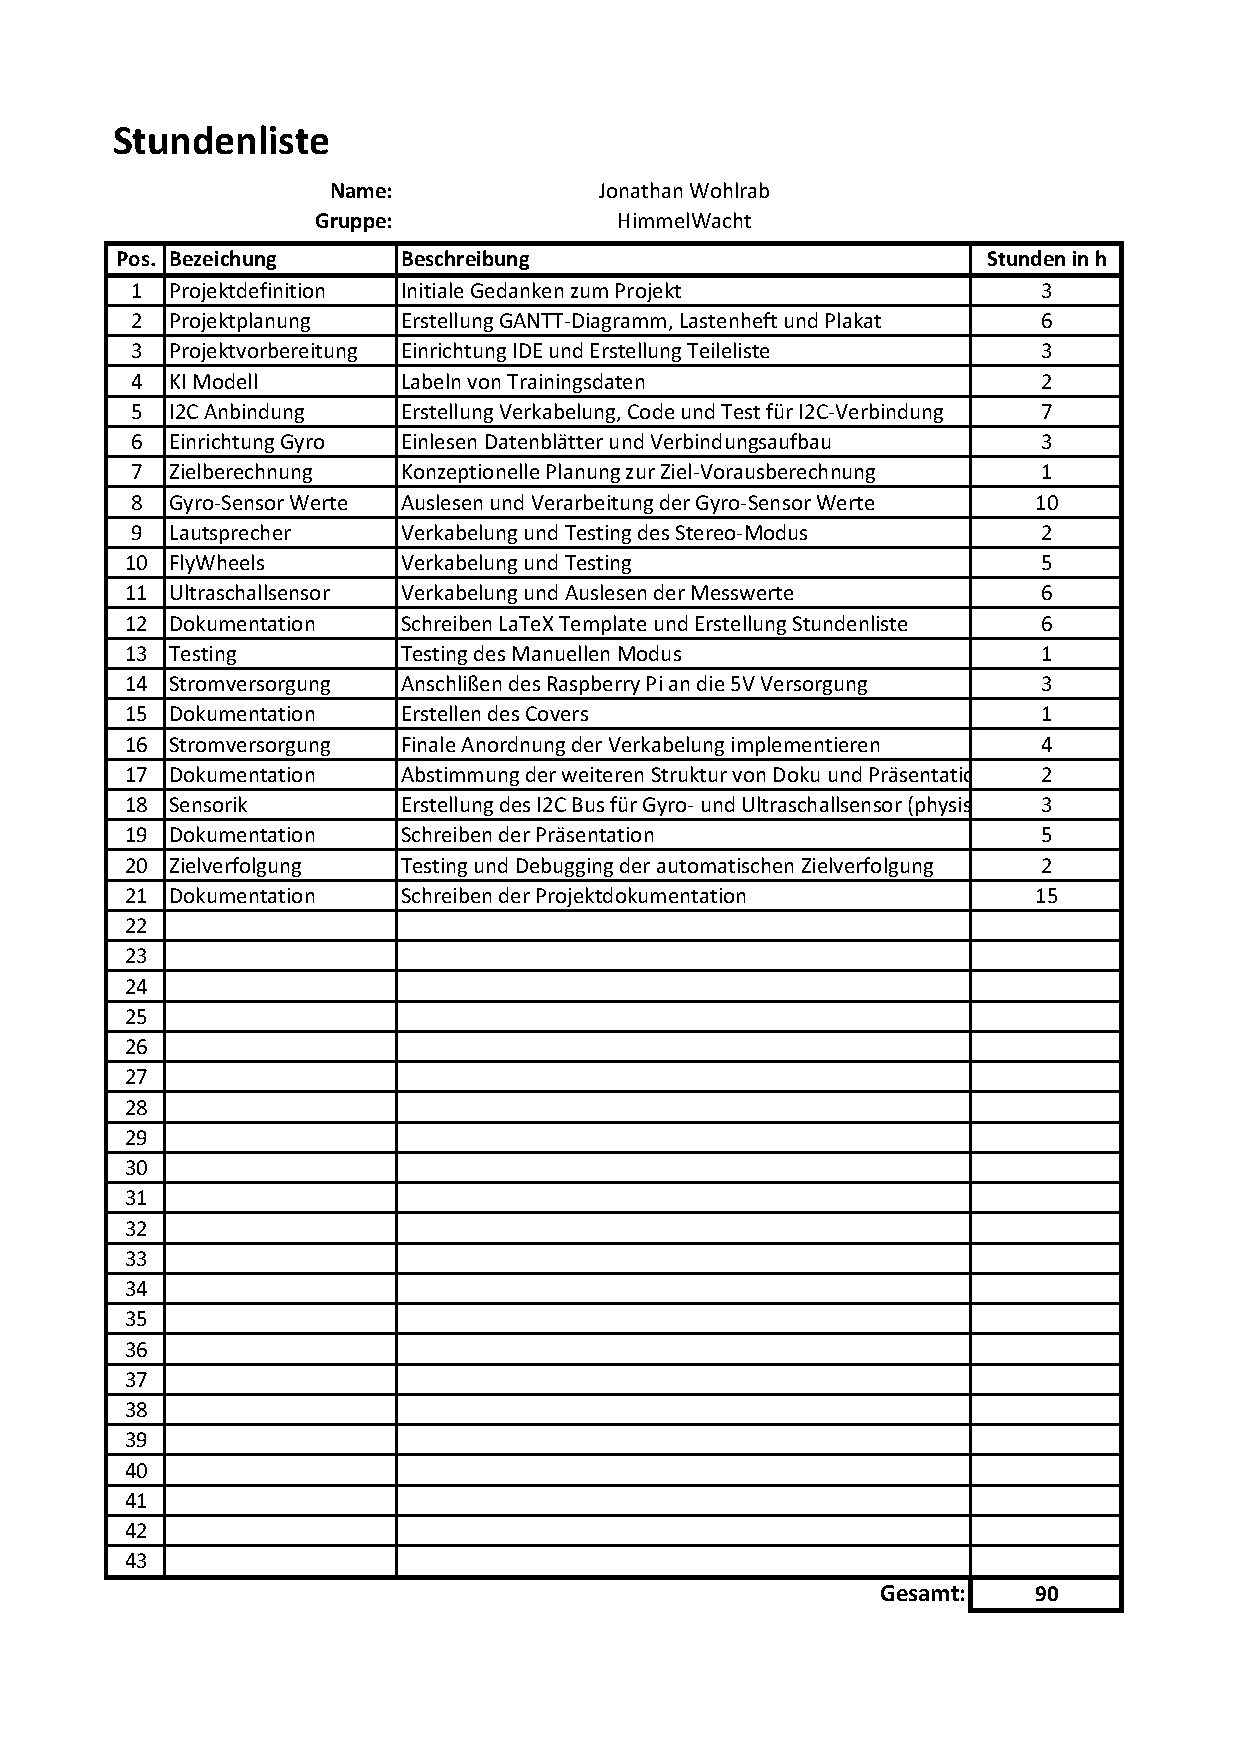
\includepdf[pages=-]{Stundenliste_Jonathan_Wohlrab.pdf}

% List of Figures
\listoffigures
\addcontentsline{toc}{chapter}{Abbildungsverzeichnis}
\newpage

% List of Tables
%\listoftables
%\addcontentsline{toc}{chapter}{Tabellenverzeichnis}
%\newpage

% List of Acronyms
%\addcontentsline{toc}{chapter}{Abkürzungen}
% \printacronyms[heading=chapter*]
%\newpage

% Bibliography
\newpage
\begin{sloppypar}
  \addcontentsline{toc}{chapter}{Literaturverzeichnis} % Add to ToC
  \printbibliography[title=Literaturverzeichnis]
\end{sloppypar}

% Annex
% \input{annex.tex}

\end{document}
